% BEGIN LICENSE BLOCK
% Version: CMPL 1.1
%
% The contents of this file are subject to the Cisco-style Mozilla Public
% License Version 1.1 (the "License"); you may not use this file except
% in compliance with the License.  You may obtain a copy of the License
% at www.eclipse-clp.org/license.
% 
% Software distributed under the License is distributed on an "AS IS"
% basis, WITHOUT WARRANTY OF ANY KIND, either express or implied.  See
% the License for the specific language governing rights and limitations
% under the License. 
% 
% The Original Code is  The ECLiPSe Constraint Logic Programming System. 
% The Initial Developer of the Original Code is  Cisco Systems, Inc. 
% Portions created by the Initial Developer are
% Copyright (C) 2006 Cisco Systems, Inc.  All Rights Reserved.
% 
% Contributor(s): 
% 
% END LICENSE BLOCK
%
%
% embroot.tex
%--------------------------------------------------------------
%
% Root file for ECLiPSe Embedding Manual
%
%--------------------------------------------------------------

%\documentstyle[11pt,html,oneside,a4wide,epsf]{book}
%\documentstyle[11pt,html,a4wide,epsf,ae,aecompl]{book}
\documentclass[11pt,a4paper]{book}
\usepackage{hevea}
\usepackage{alltt}
\usepackage{graphics}
%\usepackage{html}
\usepackage{ae}
\usepackage{aecompl}
\usepackage{makeidx}
\usepackage{tocbibind}
\usepackage{hyperref}
\topmargin -1cm
\oddsidemargin 0cm
\evensidemargin 0cm
\textwidth 16cm
\textheight 22.5cm

% Don't use a style file because latex2html ignores it
%\latex{
% trick to stop latex2html from including the file (ignore the warning!)
%\newcommand{\myinclude}[1]{\include{#1}}
%\myinclude{sepiachip}
%}

\usepackage{../texinputs/eclipse}
%\html{
%
% $Id: sepiachiphtml.tex,v 1.9 2015/10/17 03:01:33 kish_shen Exp $
%
% BEGIN LICENSE BLOCK
% Version: CMPL 1.1
%
% The contents of this file are subject to the Cisco-style Mozilla Public
% License Version 1.1 (the "License"); you may not use this file except
% in compliance with the License.  You may obtain a copy of the License
% at www.eclipse-clp.org/license.
%
% Software distributed under the License is distributed on an "AS IS"
% basis, WITHOUT WARRANTY OF ANY KIND, either express or implied.  See
% the License for the specific language governing rights and limitations
% under the License.
%
% The Original Code is  The ECLiPSe Constraint Logic Programming System.
% The Initial Developer of the Original Code is  Cisco Systems, Inc.
% Portions created by the Initial Developer are
% Copyright (C) 2006 Cisco Systems, Inc.  All Rights Reserved.
%
% Contributor(s):
%
% END LICENSE BLOCK

% This is not the original sepiachip.sty,
% but a drastically simplified one.
%

\newcommand{\eclipseversion}{6.2}

% characters for indexing ? needed for a HeVeA bug
\newcommand*{\query}{?}
\newcommand*{\atsym}{@}
\newcommand*{\cutsym}{!}

% Like index, but in tt font
\newcommand*{\indextt}[1]{\index{#1@\texttt{#1}}}

\newcommand*{\newitem}[1]{\item[#1]}

\newcommand*{\bipnoidx}[1]{\textbf{#1}}
\newcommand*{\bip}[1]{\bipnoidx{#1}\indextt{#1}}

%\newcommand{\biprefnoidx}[2]{\latex{{\bf #1}}\html{\htmladdnormallink{#1}{#2}}}
\newcommand*{\biprefnoidx}[2]{\ahref{#2}{\textbf{#1}}}
\newcommand*{\biprefni}[2]{\biprefnoidx{#1}{#2}}
\newcommand*{\bipref}[2]{\biprefnoidx{#1}{#2}\indextt{#1}}

\newcommand*{\biptxt}[2]{\bipnoidx{#1}\indextt{#2}}
\newcommand*{\txtbip}[2]{\bipnoidx{#1}\indextt{#1}}

\newcommand*{\biptxtrefni}[3]{\biprefnoidx{#1}{#3}}
\newcommand*{\biptxtref}[3]{\biprefnoidx{#1}{#3}\indextt{#2}}

\newcommand*{\txtbiprefni}[3]{\biprefnoidx{#1}{#3}}
\newcommand*{\txtbipref}[3]{\txtbiprefni{#1}{}{#3}\indextt{#1}}

% Put this word in the text, but also index it:
\newcommand*{\Index}[1]{#1\index{#1}}
% Ditto, but index in textt:
\newcommand*{\Indextt}[1]{#1\indextt{#1}}

% A word/phrase that we are talking about, not just a part of the sentence:
\newcommand*{\about}[1]{\emph{#1}}
% Ditto, with an index entry:
\newcommand*{\aboutidx}[1]{\about{#1}\index{#1}}

% Chapter name
\newcommand*{\chapname}[1]{\emph{#1}}

% Example name
\newcommand*{\examplename}[1]{\emph{#1}}

% Tool name
\newcommand*{\toolname}[1]{\emph{#1}}

% The first, defining occurrence of the name of a concept etc.:
\newcommand*{\defnotion}[1]{\textbf{#1}\index{#1}}
% Ditto with a different index entry:
\newcommand*{\defnotioni}[2]{\textbf{#1}\index{#2}}
% Ditto without an index entry:
\newcommand*{\defnotionni}[1]{\textbf{#1}}

% Concrete notation, also a very short fragment of a program embedded in the
% text, a concrete file name etc.
\newcommand*{\notation}[1]{\texttt{#1}}
% Ditto, with an index entry:
\newcommand*{\notationidx}[1]{\notation{#1}\indextt{#1}}

% A pattern, i.e., notation that is not concrete:
\newcommand*{\pattern}[1]{\textsl{#1}}
% Ditto, with an index entry:
\newcommand*{\patternidx}[1]{\pattern{#1}\index{#1@\textsl{#1}}}

% Predicate specification, i.e., name/arity
\newcommand*{\predspec}[1]{\textbf{#1}}
% Ditto with an index entry:
\newcommand*{\predspecidx}[1]{\predspec{#1}\indextt{#1}}

% Predicate ``definition'', e.g., showing it with arguments patterns.
% NOTE: have to add indextt explicitly.
\newcommand*{\preddef}[1]{\textbf{#1}}

% Index entry for a library:
\newcommand*{\libidx}[1]%
{\index{#1@\textbf{#1} (library)}\index{library!\textbf{#1}}}
% Library specification, with index:
\newcommand*{\libspec}[1]{\textbf{#1}\libidx{#1}}


% Index entry for a command line option:
\newcommand*{\cmdlineoptionidx}[1]%
{\index{command line options!\notation{-#1}}%
\index{#1 (command line option)@\notation{-#1} (command line option)}}

% Index entry for a handler:
\newcommand*{\handleridx}[1]%
{\index{#1 handler@\notation{#1} handler}\index{handler!\notation{#1}}}

% Bold table column heading etc.
\newcommand*{\heading}[1]{\textbf{#1}}



\newcommand*{\vbar}{$\mid$}
\newcommand*{\uparr}{$\wedge$}
\newcommand*{\bsl}{$\backslash$}
\newcommand*{\andsy}{$/\backslash$}
\newcommand*{\orsy}{$\backslash/$}
\newcommand*{\tld}{$\sim$}
\newcommand*{\lbr}{$[$}
\newcommand*{\rbr}{$]$}
\newcommand*{\nil}{$[~]$}
\newcommand*{\lt}{$<$}
\newcommand*{\gt}{$>$}
\newcommand*{\chr}{{\sf CHR}}
\newcommand*{\chrs}{{\sf CHR}s}
\newcommand*{\eclipse}{ECL$^i$PS$^e$}
\newcommand*{\tkeclipse}{TkECL$^i$PS$^e$}
\newcommand*{\sepia}{SEPIA}



%-------------------------------
%
% @(#)umsdebuggercomms.tex	1.3 93/03/29
%
\newenvironment{descr}[1]
{\begin{list}{}{\setlength{\leftmargin}{#1}}}{\end{list}}

% Index entry for a debugger command:
\newcommand*{\dbgcmdidx}[2]{\dbgcmdidxPlus{#1}{#1}{#2}}
% Ditto when the indexing entry is different from the one shown,
% e.g., \dbgcmdidxPlus{$<$}{<}{print depth}:
\newcommand*{\dbgcmdidxPlus}[3]%
{\index{#1---#3 (debugger cmd)@\notation{#2}---#3 (debugger cmd)}%
\index{debugger command!\notation{#2}}}

\newcommand*{\cmd}[2]%
{\item[\textbf{#1}\hfill]\textbf{#2}\dbgcmdidx{#1}{#2}}

\newcommand*{\ncmd}[2]{\item[\textit{n} \textbf{#1}\hfill]\textbf{#2}%
\dbgcmdidx{#1}{#2}}

\newcommand*{\mcmd}[2]{\mcmdPlus{#1}{#1}{#2}}

\newcommand*{\mcmdPlus}[3]{\item[\textbf{#1} \textit{par}\hfill]\textbf{#3}%
\dbgcmdidxPlus{#1}{#2}{#3}}

\newcommand*{\nmcmd}[2]{\item[{\it n\bf #1 {\it par}} \hfill] {\bf #2}%
\dbgcmdidx{#1}{#2}}
%-------------------------------


\let\ifonline=\iffalse

%}
\tolerance=10000

%--------------------------------------------------------------

\makeindex

%--------------------------------------------------------------

\title{
    {\Large\bf \eclipse}\\
    \vspace{1cm}
    {\Huge\bf Embedding and Interfacing Manual}\\
    \vspace{1cm}
    Release \eclipseversion}

\author{
Stefano Novello (IC-Parc) \\
Joachim Schimpf (IC-Parc) \\
Kish Shen       (IC-Parc) \\
Josh Singer	(Parc Technologies Ltd.)
}

\begin{document}


\maketitle

%--------------------------------------------------------------

% Needed to adjust left/right pages properly
\setcounter{page}{2}
% Suppress printing of the page number on this page
\pagestyle{empty}

\vfill
\noindent{\LARGE\bf Trademarks}

\bigskip\bigskip
WindowsNT and Windows95 are trademarks of Microsoft Corp.

Java, SunOS and Solaris are trademarks of Sun Microsystems, Inc.

\copyright\ 1996 -- 2006 Cisco Systems, Inc
\bigskip\bigskip\bigskip\bigskip\bigskip\bigskip

%--------------------------------------------------------------
\cleardoublepage
\pagestyle{plain}
\pagenumbering{roman}

\tableofcontents

%--------------------------------------------------------------
\cleardoublepage
\pagenumbering{arabic}

\chapter{Introduction}
This manual contains the information needed to interface {\eclipse}
code to C, C++ or Java environments, or to use it from within scripting
languages such as Tcl.
{\eclipse} is available in the form of a linkable library,
and a number of facilities are available to pass data between the
different environments, to make the integration as close as possible.

It also contains information on interfacing to external software systems,
such as database management systems.

Example sources can be found in the {\eclipse} installation directory
under \bipref{doc/examples}{../examples}.

% BEGIN LICENSE BLOCK
% Version: CMPL 1.1
%
% The contents of this file are subject to the Cisco-style Mozilla Public
% License Version 1.1 (the "License"); you may not use this file except
% in compliance with the License.  You may obtain a copy of the License
% at www.eclipse-clp.org/license.
% 
% Software distributed under the License is distributed on an "AS IS"
% basis, WITHOUT WARRANTY OF ANY KIND, either express or implied.  See
% the License for the specific language governing rights and limitations
% under the License. 
% 
% The Original Code is  The ECLiPSe Constraint Logic Programming System. 
% The Initial Developer of the Original Code is  Cisco Systems, Inc. 
% Portions created by the Initial Developer are
% Copyright (C) 2006 Cisco Systems, Inc.  All Rights Reserved.
% 
% Contributor(s): 
% 
% END LICENSE BLOCK
%
% @(#)umscmacros.tex    
%

%%%%%%%%%%%%%%%%%%%%%%%%%%%%%%%%%%%%%%%%%%%%%%%%%%%%%%%%%%%%%%%%%%%%%%%%%%
% {\eclipse} Documentation
%
% embed.tex
%
%%%%%%%%%%%%%%%%%%%%%%%%%%%%%%%%%%%%%%%%%%%%%%%%%%%%%%%%%%%%%%%%%%%%%%%%%%
\chapter{Calling {\eclipse} from  C++}
\label{chap1embed}
%HEVEA\cutdef[1]{section}

This chapter describes how {\eclipse} can be included in an external
program as a library, how to start it, and how to
communicate with it. Code examples are given in C++.
For the equivalent C functions, please refer to chapter~\ref{chapsumc}.

%---------------------------------------------------------------------
\section{To get started}
%---------------------------------------------------------------------

This section is about the prerequisites for working with
{\eclipse} in your development environment. The directory structure,
the libraries and the include files are described.

\subsection{Directories}
\index{directories}

The libraries and include files needed to use {\eclipse} as an
embedded component are available under the {\eclipse}
\index{installation directory}
directory which was set-up during installation. If you have access
to a stand-alone {\eclipse} it can be found using the following query
at the {\eclipse} prompt:

\begin{verbatim}
    [eclipse 1]: get_flag(installation_directory,Dir).

    Dir = "/usr/local/eclipse"
    yes.
    [eclipse 2]
\end{verbatim}

We will assume from here that {\eclipse} was installed in "/usr/local/eclipse".

You would find the include files in "/usr/local/eclipse/include/\$ARCH"
and the the libraries in "/usr/local/eclipse/lib/\$ARCH" where
"\$ARCH" is a string naming the architecture of your machine.
\index{ARCH}
\index{architecture}
This can be found using the following {\eclipse} query:

\begin{verbatim}
    [eclipse 2]: get_flag(hostarch,Arch).

    Arch = "sun4"
    yes.
    [eclipse 3]:
\end{verbatim}

You will need to inform your C or C++ compiler and linker about these
directories so that these tools can include and link the appropriate files.
A make file "Makefile.external" can be found together with the libraries.
\index{Makefile}
The definitions in that makefile may  have to be updated according to
your operating system environment.

A set of example C and C++ programs can be found in
"/usr/local/eclipse/doc/examples".

When delivering an application you will have to include with it the
contents of the directory 
"/usr/local/eclipse/lib" without which {\eclipse}
cannot work. Normally this would be copied into the directory structure
of the delivered application. The interface can set different values
for this directory, enabling different applications to have different
sets of libraries.


\subsection{Definitions}

To include the definitions needed for calling the {\eclipse} library
in a C program use:
\index{include files}
\begin{verbatim}
    #include <eclipse.h>
\end{verbatim}

For C++ a more convenient calling convention can be used based on
some classes wrapped around these C definitions. To include these use:

\begin{verbatim}
    #include <eclipseclass.h>
\end{verbatim}



\subsection{Compiling, linking and running on Unix/Linux}

Assuming that the environment variable ECLIPSEDIR is set to the
{\eclipse} installation directory and the environment variable ARCH is set to
the architecture/operating system name,
an application can be built as follows:
\begin{verbatim}
gcc -I$ECLIPSEDIR/include/$ARCH eg_c_basic.c -L$ECLIPSEDIR/lib/$ARCH -leclipse
\end{verbatim}
This will link your application with the shared library \verb+libeclipse.so+.

At runtime, your application must be able to locate \verb+libeclipse.so+.
This can be achieved by adding $ECLIPSEDIR/lib/$ARCH to your
\verb+LD_LIBRARY_PATH+ environment variable.

The embedded {\eclipse} finds its own support files (e.g.\ {\eclipse} libraries)
through the \verb+ECLIPSEDIR+ environment variable.
This must be set to the location where {\eclipse} is installed,
e.g.\ \verb+/usr/local/eclipse+.
Alternatively, the application can invoke \verb+ec_set_option+ to specify
the \verb+ECLIPSEDIR+ location before initialising the embedded {\eclipse}
with \verb+ec_init+.


%\subsection{Static linking (Unix/Linux)}
%
%If your operating system only supports static linking, or if you want
%to link statically for some reason, you have to link explicitly with
%\verb+libeclipse.a+ and the necessary support libraries must be specified, e.g.
%\begin{verbatim}
%gcc -I$ECLIPSEDIR/include/$ARCH eg_c_basic.c $ECLIPSEDIR/lib/$ARCH/libeclipse.a
%    -L$ECLIPSEDIR/lib/$ARCH -lgmp -lshm -ldummies -ldl -lnsl -lsocket -lm
%\end{verbatim}
%The libraries \verb+gmp+, \verb+shm+ and \verb+dummies+ are {\eclipse}
%support libraries and must be specified in that order.
%The others are Unix libraries.
%
%It is recommended that you copy the makefile "Makefile.external"
%provided in your  installation directory under lib/\$ARCH and adapt it
%for your purposes.
%\index{Makefile}
% If the makefile is not used, the command to compile a C++ source
% with {\eclipse} library calls looks similar to this:
% \begin{verbatim}
%     % g++ -I/usr/local/eclipse/include/sparc_sunos5 -c eg_cc_main.cc
% \end{verbatim}
% The linking of an executable with embedded {\eclipse} looks like
% \begin{verbatim}
%     % g++ eg_cc_main.o -L/usr/local/eclipse/lib/sparc_sunos5 -leclipse
%                        -lgmp -lshm -ldummies -ldl -lnsl -lsocket -lm
% \end{verbatim}
% The details may vary depending on what compiler and operating system
% you use.  Refer to the Makefile.external for details.


\subsection{Compiling, linking and running on Windows}

If you use GCC, you can link either directly against \verb+eclipse.dll+
or against \verb+eclipse.dll.a+.
The required command line is similar to the Unix case.

If you use a Microsoft compiler, make sure you have the following
additional settings in your C/C++ compiler/development system:
\begin{itemize}
\item In the {\bf C/C++ Preprocessor} settings,
specify the {\eclipse} include directory as an additional
include directory, e.g.\ \verb+C:\Program Files\ECLiPSe 5.10\include\i386_nt+.
\item In the {\bf Link} settings,
specify \verb+eclipse.lib+ as an additional object/library
module, and the location of this library, e.g.\
\verb+C:\Program Files\ECLiPSe 5.10\lib\i386_nt+ as an additional library path.
\end{itemize}
\index{eclipse.lib}
Moreover, you need to create an \verb+eclipse.lib+ for the compiler to
link against.  This file can be created from \verb+eclipse.def+ and
\verb+eclipse.dll+ (which are part of the {\eclipse} distribution),
using the \verb+lib.exe+ or \verb+link.exe+ tool (which comes with the
C/C++ development system).
\begin{verbatim}
    cd C:\Program Files\ECLiPSe 5.10\lib\i386_nt
    lib.exe /def:eclipse.def
\end{verbatim}
Warnings about import directives can be ignored.
If you do not have \verb+lib.exe+, try instead
\begin{verbatim}
    link.exe /lib /def:eclipse.def
\end{verbatim}

At runtime, your application must be able to locate \verb+eclipse.dll+,
\index{eclipse.dll}
i.e.\ you should either
\begin{itemize}
\item copy \verb+eclipse.dll+ into the folder where your application is located, or
\item copy \verb+eclipse.dll+ into one of Windows' standard library folders, or
\item add the path to the folder where \verb+eclipse.dll+ can be found
	to your PATH environment variable.
\end{itemize}
The \verb+eclipse.dll+ finds its own support files (e.g.\ {\eclipse} libraries)
through the \verb+ECLIPSEDIR+ registry entry under the registry key
\verb+HKEY_LOCAL_MACHINE\SOFTWARE\IC-Parc\ECLiPSe\X.Y+ (X.Y is the version
number).
This must be set to the location where {\eclipse} is installed,
e.g.\ \verb+C:/Eclipse+.
Alternatively, the application can invoke \verb+ec_set_option+ to specify
the \verb+ECLIPSEDIR+ location before initialising the embedded {\eclipse}
with \verb+ec_init+.


%---------------------------------------------------------------------
\section{Creating an {\eclipse} context}
%---------------------------------------------------------------------

{\eclipse} runs as a special thread (we will call it {\eclipse} engine) within
your application,
maintaining its own execution state. This section is about when and
how to initialise it. There are parameters to be applied before
initialisation, but these are usually acceptable. These parameters are
described in Appendix~\ref{chapecoptions}.

Although it is useful to think of {\eclipse} as a thread, it is not an
\index{thread}
operating system thread, but is rather implemented as a set of C
functions that maintain some state. This state is the complete
execution state of the {\eclipse} engine, its stack of goals, its
success and failure continuations and its global stack of all
constructed data.

At particular points during its execution {\eclipse} will yield control
back to the C level. This is implemented by returning from a function.
{\eclipse} can then be restarted from the exact point it left off. This
is implemented by a function call.

\subsection{Initialisation}

You initialise {\eclipse} by calling the parameterless function
\index{initialisation}
\begin{verbatim}
    int ec_init();
\end{verbatim}

A process should do this just once. \verb.ec_init. returns 0 on success or
-1 if an error occurred. It is possible to influence the initialisation of
{\eclipse} by setting initialisation options as described in
Appendix~\ref{chapecoptions}.

None of the functions of the interface work before this initialisation. In
particular in C++, if you use static variables which are
constructed by calling {\eclipse} functions you must arrange for the
initialisation to occur before the constructors are called.


%---------------------------------------------------------------------
\section{Control flow}
%---------------------------------------------------------------------

{\eclipse} and a C or C++ main program are like threads running in a
single process. Each maintains its state and methods for exchanging
\index{thread}
\index{state}
data and yielding control to the other thread.

The main method of sending data from C++ to {\eclipse} is by posting
\index{posting goals}
goals for it to solve. All posted goals are solved in conjunction
with each other, and with any previously posted goals that have
succeeded.

Data is passed back by binding logical variables within the goals.
\index{logical variable}

\index{resume}
Control is explicit in C++. After posting some goals, the C++ program
calls the \verb.EC_resume(). function and these goals are all
solved. A return code says whether they were successfully solved
or whether a failure occurred.


In {\eclipse} control is normally implicit. Control returns to C++ when all
goals have been solved.

\begin{verbatim}
    #include        "eclipseclass.h"

    main()
    {
        ec_init();

        /* writeln("hello world"), */
        post_goal(term(EC_functor("writeln",1),"hello world"));
        EC_resume();
        ec_cleanup(0);
    }
\end{verbatim}
The above is an example program that posts a goal and executes it.

\subsection{Control flow and search}

Using this model of communication it is possible to construct programs where
execution of C++ code and search within the {\eclipse} are interleaved.

\index{posting goals}
\index{failure}
\index{backtracking}
If you post a number of goals (of which some are non-deterministic) and
resume the {\eclipse} execution and the goals succeed, then control returns
to the C++ level. By posting a goal that fails, the {\eclipse} execution
will fail back into the previous set of goals and these will succeed with
a different solution. 

\begin{verbatim}
    #include        "eclipseclass.h"

    main()
    {
        ec_init();
        EC_ref Pred;

        post_goal(term(EC_functor("current_built_in",1),Pred));
        while (EC_succeed == EC_resume())
        {
            post_goal(term(EC_functor("writeln",1),Pred));
            post_goal(EC_atom("fail"));
        }
        ec_cleanup(0);
    }
\end{verbatim}
The above example prints all the built ins available in {\eclipse}.
When \verb.EC_resume(). returns \verb.EC_succeed. there is a solution
to a set of posted goals, and we print out the value of \verb.Pred..
otherwise \verb.EC_resume(). returns \verb.EC_fail. to indicate
that no more solutions to any set of posted goals is available.

\index{cut}
It is possible also to cut such search. So for example one could modify
the example above to only print the 10th answer. Initially one simply
fails, but at the tenth solution one cuts further choices. Then
one prints the value of 'Pred'.

\begin{verbatim}
    #include        "eclipseclass.h"

    main()
    {
        ec_init();
        EC_ref Pred,Choice;
        int i = 0;

        post_goal(term(EC_functor("current_built_in",1),Pred));
        while (EC_succeed == EC_resume(Choice))
        {
            if (i++ == 10)
            {
                Choice.cut_to();
                break;
            }
            post_goal(term(EC_atom("fail")));
        }
        post_goal(term(EC_functor("writeln",1),Pred));
        EC_resume():
        ec_cleanup(0);
    }
\end{verbatim}

\index{choicepoint}
When \verb.EC_resume(). is called with an \verb.EC_ref. argument, this
is for data returned by the \verb.EC_resume(). If the return code is
\verb.EC_succeed. The \verb.EC_ref. is set to a choicepoint identifier
which can be used for cutting further choices at that point.

\subsection{Asynchronous events}

\index{events}
\index{posting events}
The posting of goals and building of any {\eclipse} terms in general
cannot be done asynchronously to the {\eclipse} execution. It has to
be done after the \verb.EC_resume(). function has returned.

\index{asynchronous}
Sometimes it may be necessary to signal some asynchronous event to
{\eclipse}, for example to implement a time-out. To do this one
posts a named event to {\eclipse}. At the next synchronous point
within the eclipse execution, the handler for that event is
invoked.
\begin{verbatim}
    /* C++ code, possibly within a signal handler */
    post_event(EC_atom("timeout"));

    /* ECLiPSe code */
    handle_timeout(timeout) :-
        <appropriate action>

    :- set_event_handler(timeout, handle_timeout/1).
\end{verbatim}


\subsection{The yield-resume model}

\index{passing data}
\index{yield}
\index{resume}
Although implicitly yielding control when a set of goals succeeds
or fails is often enough, it is possible to explicitly yield
control to the C++ level. This is done with the
\bipref{yield/2}{../bips/kernel/externals/yield-2.html}
predicate.  This yields control to the calling C++ program.
The arguments are used for passing data to C++ and from C++.

When \bipref{yield/2}{../bips/kernel/externals/yield-2.html} is called within {\eclipse} code, the \verb.EC_resume().
function returns the value \verb.EC_yield. so one can recognise this case.
The data passed out via the first argument of \bipref{yield/2}{../bips/kernel/externals/yield-2.html}
can  be accessed from C++ via the \verb.EC_ref. argument to \verb.EC_resume()..
The data received in the second argument of \bipref{yield/2}{../bips/kernel/externals/yield-2.html} is either
the list of posted goals, or an \verb.EC_word. passed as an input
argument to \verb.EC_resume()..

\begin{verbatim}
    yield(out(1,2),InData),
\end{verbatim}

In this example the compound term \verb.out(1,2). is passed to C++.
If we had previously called:
\begin{verbatim}
    EC_ref FromEclipse;
    result = EC_resume(FromEclipse);
\end{verbatim}
then \verb.result. would be \verb.EC_yield. and \verb.FromEclipse. would
refer to \verb.out(1,2).. If then we resumed execution with:
\begin{verbatim}
    result = EC_resume(EC_atom("ok"),FromEclipse);
\end{verbatim}
then the variable \verb.InData. on the {\eclipse} side
would be set to the atom 'ok'.


\subsection{Summary of EC_resume() arguments}

\index{passing data}
\verb.EC_resume(). can be called with two optional arguments. An
input argument that is an \verb.EC_word. and an output that is an
\verb.EC_ref..

If the input argument is omitted, input is taken as the list of posted
goals. Otherwise the input to {\eclipse} is exactly that argument.

If the output argument is present, its content depends on the value
returned by \verb.EC_resume().. If it returns \verb.EC_succeed. it is
\index{choicepoint}
the choicepoint identifier. If it returns \verb.EC_yield. It is the
first argument to the  \bipref{yield/2}{../bips/kernel/externals/yield-2.html} goal. If it returns \verb.EC_fail.
it is not modified.
%HEVEA\cutend


%---------------------------------------------------------------------
\chapter{Managing Data and Memory in Mixed-Language Applications}
\label{chapmixed}
%HEVEA\cutdef[1]{section}
%---------------------------------------------------------------------

{\eclipse} is a software engine for constraint propagation and search tasks.
As such, it represents its data in a form that is different
from how it would be represented in a traditional C/C++ program.
\index{search}
\index{garbage collection}
\index{memory management}
In particular,
the {\eclipse} data representation supports automatic memory management
and garbage collection, modifications that can be undone in a search context,
referential transparency and dynamic typing.

In a mixed-language application, there are two basic ways of communicating
information between the components coded in the different languages:
\index{passing data}
\begin{description}
\item[Conversion:] When data is needed for processing in another language,
        it can be converted to the corresponding representation.
        This technique is appropriate for simple data types (integers, strings),
        but can have a lot of overhead for complex structures.
\item[Sharing:] The bulk of the data is left in its original representation,
        referred to by a handle, and interface functions (or methods) provide
        access to its components when required.
\end{description}
Both techniques are supported by the {\eclipse}/C and {\eclipse}/C++ interface.


%--------------------------------
\section{Constructing {\eclipse} data}
%--------------------------------
\subsection{{\eclipse} atoms and functors}

\index{passing data}
\index{atom}
\index{functor}
\begin{verbatim}
    /* ECLiPSe code */
    S = book("Gulliver's Tales","Swift",hardback,fiction),
\end{verbatim}

In the above structure 'hardback' and 'fiction' are atoms. 'book'
is the functor of that structure, and it has an arity (number
of arguments) of 4.

Each functor and atom is entered into a dictionary, and is always
referred to by its dictionary entry. Two classes, \verb.EC_atom.
and \verb.EC_functor. are used to access such dictionary entries.

The 'Name' method applies to both, to get their string form.
The 'Arity' method can be used to find out how many arguments
a functor has.

\begin{verbatim}
    /* C++ code */
    EC_functor book("book",4);
    EC_atom hardback("hardback");

    if (book.Arity()) == 4) .. /* evaluates to true */
    if (book == hardback) ..   /* evaluates to false */
    s = hardback.Name();       /* like s = "hardback"; */
\end{verbatim}


\subsection{Building {\eclipse} terms}

\index{pword}
\index{EC_word}
\index{term}
The \verb.pword. C data type is used to store {\eclipse} terms. In C++ the
\verb.EC_word. data type is used. This is used for any C type as well
as for {\eclipse} structures and lists. The size remains fixed in all
cases, since large terms are constructed on the {\eclipse} global stack.

\index{garbage collection}
The consequences of this are that terms will be garbage collected
or moved so terms do not survive the execution of {\eclipse}. In
particular, one cannot build such terms asynchronously while
{\eclipse} is running, for example this precludes building terms from
within a signal handler unless it can make sure that {\eclipse} has
yielded when it is running.

\subsection{Building atomic {\eclipse} terms}
It is possible to simply cast from a number of simple C++ types to
build an \verb.EC_word. In addition, functions exist for creating
\index{logical variable}
new variables, and for the nil which terminates {\eclipse} lists.
In C++ you can just cast.
\begin{verbatim}
    /* making simple terms in C++ */
    EC_word w;
    EC_atom hardback("hardback");
    w = (EC_word) "Swift";
    w = (EC_word) hardback;
    w = (EC_word) 1.002e-7;
    w = (EC_word) 12345;
    w = (EC_word) nil();
    w = (EC_word) newvar();

    /* ECLiPSe equivalent code */
    P1 = "Swift",
    P2 = hardback,
    P3 = 1.002e-7,
    P4 = 12345,
    P5 = [],
    P6 = _,
\end{verbatim}

\subsection{Building {\eclipse} lists}
\index{list}
The \verb.list(head,tail). function builds a list out of two terms. Well
formed lists have lists as their tail term and a nil ("[]") at the end, or a
variable at the end for difference lists.

\begin{verbatim}
    /* making the list [1, "b", 3.0] in C++ */
    EC_word w = list(1, list("b", list(3.0, nil())));
\end{verbatim}

The following example shows how you can write functions to build
variable length lists.

\begin{verbatim}
/* function to build a list [n,n+1,n+2,.....,m-1,m] */
EC_word fromto(int n, int m)
{
    EC_word tail = nil();
    for(int i = m ; i >= n ; i--)
        tail = list(i,tail);
    return tail;
}
\end{verbatim}

The list is constructed starting from the end, so at all points during its
construction you have a valid term. The interface is designed to
make it hard to construct terms with uninitialised sub-terms, which is
what you would need if you were to construct the list starting with
the first elements.

\subsection{Building {\eclipse} structures}
\index{term}
\index{structure}
\index{compound term}
The \verb%term(functor,args..)% function is used to build {\eclipse}
structures. A number of different functions each with a different
number of arguments is defined so as not to disable C++ casting
which would be the case if we defined a function with variable
arguments.

\begin{verbatim}
    /* making s(1,2,3) in C++ */
    EC_functor s_3("s",3);
    EC_word w = term(s_3,1,2,3);
\end{verbatim}

The above interface is convenient for terms with small fixed arities,
for much larger terms an array based interface is provided.

\begin{verbatim}
    /* making s(1,2,..,n-1,n) */
    EC_word args[n];
    for(int i=0 ; i<n ; i++)
        args[i] = i+1;
    EC_word w = term(EC_functor("s",n),args);
\end{verbatim}


%--------------------------------
\section{Converting {\eclipse} data to C data}
%--------------------------------

\index{type testing}
There are several aspects to examining the contents of a term. These
include decomposing compound terms such as lists and structures,
converting simple terms to C data types and testing the types of terms.

The functions for decomposing and converting check that the type
is appropriate. If it is they return \verb.EC_succeed. if not
they return a negative error code.

\subsection{Converting simple {\eclipse} terms to C data types}

To convert from an {\eclipse} term to a C type you first have to
declare a variable with that type. For fixed size data types
(you can convert to \verb.double., \verb.long. and \verb.dident.
fixed size data types) you are responsible for allocating the
memory. For strings you declare a \verb.char*. variable and
on conversion it will point to the internal {\eclipse} string.
\index{string}

In the following example we see how one can try to convert to
different types. Of course normally you will know what type
you are expecting so only one of these functions need be called.
\begin{verbatim}
    EC_word term;
    double r;
    long i;
    EC_atom did;
    char *s;
    if (EC_succeed == term.is_double(&d))
        cout << d << "\n";
    else if (EC_succeed == term.is_long(&i))
        cout << i << "\n";
    else if (EC_succeed == term.is_atom(&did))
        cout << did.Name() << "\n";
    else if (EC_succeed == term.is_string(&s))
        cout << s << "\n";
    else
        cout << "not a simple type\n";
\end{verbatim}

The term is converted by the function which returns \verb.EC_success..
The functions that fail to convert will return a negative error number.

\index{string}
\index{garbage collection}
Care has to be taken with strings, these pointers point to the internal
{\eclipse} string which may move or be garbage collected during an {\eclipse}
execution. As a result if a string is to be kept permanently one should
copy it first.


\subsection{Decomposing {\eclipse} terms}

The function \verb.ec_get_arg(index,term,&subterm). is used to get
the index'th subterm of a structure. The index varies from 1 to
arity of \verb.term.. A list can also be decomposed this way, where
the head is at index 1 and the tail at index 2.
\index{list}
\index{structure}

Below we see how we would write a function to find the nth element of
a list.
\begin{verbatim}
    int nth(const int n,const EC_word list, EC_word& el)
    {
        EC_word tail = list;
        for (int i=1, i<n, i++)
            if (EC_fail == tail.arg(2,tail))
                return EC_fail;
        return tail.arg(1,el);
    }
\end{verbatim}
The above function actually is not limited to lists but could work
on any nested structure.


%--------------------------------
\section{Referring to {\eclipse} terms}
%--------------------------------

The terms constructed so far (as EC-words) have been volatile, that is they
do not survive an {\eclipse} execution (due to eg.\ garbage collection),
\index{garbage collection}
It is possible to create safe terms
that have been registered with the {\eclipse} engine and which do
survive execution. The \verb.EC_ref.  and \verb.EC_refs. classes
are provided for this purpose. \verb.EC_refs. are vectors of
safe terms.

When you declare an \verb.EC_ref. it will contain free variables.
\begin{verbatim}
EC_ref X; /* declare one free variable */
EC_refs Tasks(10); /* declare 10 free variables */
\end{verbatim}


\index{logical variables}
\verb.EC_ref.s work like logical variables. When {\eclipse} fails during search
they are reset to old values. They are always guaranteed to refer to
something i.e.\ they never contain dangling references.
If {\eclipse} backtracks to a point in the execution
older than the point at which the references were created, they
return to being free variables, or take on their initial values.

\index{references}
It is possible to declare references, giving them an initialiser
but this must be an atomic type that fits into a single word. That
restricts you to atoms, integers and nil.

You can freely assign between an \verb.EC_ref. and a \verb.EC_word..

One point to take care of is that assigning such a variable
is not like unification since assignment cannot fail. It
just overwrites the old value. Assignment is very similar
to the \bipref{setarg/3}{../bips/kernel/termmanip/setarg-3.html} built-in in the {\eclipse} language.


%---------------------------------------------------------------------
\section{Passing generic C or C++ data to {\eclipse}}
%---------------------------------------------------------------------

\index{references}
It is possible to include any C or C++ data in an {\eclipse} term. To do this
it is wrapped into a handle to tell {\eclipse} that this is external data.
You also have to supply a method table, which is a set of functions
that are called when {\eclipse} wants to make common operations that it
assumes can be done on any data (eg.\ comparing, printing).


\subsection{Wrapping and unwrapping external data in an {\eclipse} term}

To create an {\eclipse} wrapper for a C/C++ object,
the function \verb.handle(). is used. It takes a pointer to any C or C++
data, and a pointer to a suitable method table (\verb.t_ext_type. structure)
and creates an {\eclipse} handle term which refers to them.
Method tables for the common case of arrays of char, long or double
\index{array}
are predefined. For example a handle for a double array is made like this
\begin{verbatim}
    double my_array[5] = {1.1, 2.2, 3.3, 4.4, 5.5};
    EC_word w = handle(&ec_xt_double_arr, my_array);
\end{verbatim}
where \verb.ec_xt_double_arr. is a predefined method table for arrays of doubles.
To convert back from an {\eclipse} term \verb.is_handle(). is used.
The method table passed in indicates the sort of data you expect to get.
If the {\eclipse} handle contains the wrong sort, the function returns
TYPE_ERROR:
\begin{verbatim}
    if ((EC_succeed == w.is_handle(&ec_xt_double_arr, &obj))
        obj->my_method();
    else
        cerr << "unexpected type\n";
\end{verbatim}

The creation of the handle copies the address of the array, rather than the
array itself, so the handle must be used within the scope of the array.

\subsection{The method table}
\index{method table}
Apart from the predefined method tables ec_xt_double_arr,
ec_xt_long_arr and ec_xt_char_arr, new ones can easily be defined.
The address of the table is used as a type identifier, so when you
get an external object back from {\eclipse} you can check its type
to determine the kinds of operations you can do on it.
You can choose not to implement one or more of these functions, by
leaving a null pointer (\verb.(void*)0.) in its field.

\begin{verbatim}
    typedef void *t_ext_ptr;

    typedef struct {
        void       (*free)       (t_ext_ptr obj);
        t_ext_ptr  (*copy)       (t_ext_ptr obj);
        void       (*mark_dids)  (t_ext_ptr obj);
        int        (*string_size)(t_ext_ptr obj, int quoted);
        int        (*to_string)  (t_ext_ptr obj, char *buf, int quoted);
        int        (*equal)      (t_ext_ptr obj1, t_ext_ptr obj2);
        t_ext_ptr  (*remote_copy)(t_ext_ptr obj);
        EC_word    (*get)        (t_ext_ptr obj, int idx);
        int        (*set)        (t_ext_ptr obj, int idx, EC_word data);
    } t_ext_type;
\end{verbatim}

\begin{description}
\item[void free(t_ext_ptr obj)]
\index{references}
This is called by {\eclipse} if it loses a reference to the external
data. This could happen if the {\eclipse} execution were to fail
to a point before the external object was created, or if a
permanent copy was explicitly removed with built-ins like
\bipref{setval/2}{../bips/kernel/storage/setval-2.html},
\bipref{erase/2}{../bips/kernel/record/erase-2.html}
or \bipref{bag_dissolve/2}{../bips/kernel/storage/bag_dissolve-2.html}.
Note that an invocation of this function only means that {\em one}
reference has been deleted (while the copy function indicates that
a reference is added).

\item[t_ext_ptr copy(t_ext_ptr obj)]
This is called by {\eclipse} when it wants to make a copy of an object.
This happens when calling {\eclipse} built-ins like \bipref{setval/2}{../bips/kernel/storage/setval-2.html} or
\bipref{recordz/2}{../bips/kernel/record/recordz-2.html} which make permanent copies of data. The return value is
the copy.
If no copy-method is specified, these operations will not be possible
with terms that contain an object of this type.
A possible implementation is to return a pointer to the original and
e.g.\ increment a reference counter (and decrement the counter in
the free-method correspondingly).

\item[void mark_dids( t_ext_ptr obj)]
This is called during dictionary garbage collection. If an external
object contains references to the dictionary (\verb.dident.) then
it needs to mark these as referenced.

\item[int string_size(t_ext_ptr obj, int quoted)]
\item[int to_string(t_ext_ptr obj,char *buf, int quoted)]
When {\eclipse} wants to print an external object it calls \verb.string_size().
to get an estimate of how large the string would be that represents it.
This is used by {\eclipse} to allocate a buffer. The string representation must
be guaranteed to fit in the buffer.

Finally  the \verb.to_string(). function is called. This should write the
string representation of the object into the buffer, and return the actual
size of that string.

\item[int equal(t_ext_ptr obj1, t_ext_ptr obj2)]
This is called when two external objects are unified or compared.
Prolog views the external object as a ground, atomic element.
It should return non-zero if the objects are considered equal.

\item[t_ext_ptr remote_copy(t_ext_ptr obj)]
This is called by parallel {\eclipse} when it needs to make a copy of an
object in another worker. If the object is in shared memory, this method
can be the same as the copy method.

\item[EC_Word get(t_ext_ptr obj, int idx)]
Returns the value of a field of the C/C++ object.
This methods gets invoked when the {\eclipse} predicate \bipref{xget/3}{../bips/kernel/externals/xget-3.html} is called.
The get/set method pair determines the mapping of index values to fields.

\item[int set(t_ext_ptr obj, int idx, EC_word data)]
Set the value of a field of the C/C++ object.
This methods gets invoked when the {\eclipse} predicate \bipref{xset/3}{../bips/kernel/externals/xset-3.html} is called.
The get/set method pair determines the mapping of index values to fields.
\end{description}

Example of the simplest possible user-defined method table:
\begin{verbatim}
    /* the initializer is actually not needed, NULLs are the default */
    t_ext_type my_type = {NULL,NULL,NULL,NULL,NULL,NULL,NULL,NULL,NULL};
    my_struct data_in;
    ...
    // creating a handle for data_in
    EC_word w = handle(&my_type, &data_in);
    ...
    // checking a handle and extracting the data pointer
    my_struct *data_out;
    if ((EC_succeed == w.is_handle(&my_type, &data_out))
        data_out->my_method();
    else
        cerr << "unexpected type\n";
\end{verbatim}

%HEVEA\cutend



% BEGIN LICENSE BLOCK
% Version: CMPL 1.1
%
% The contents of this file are subject to the Cisco-style Mozilla Public
% License Version 1.1 (the "License"); you may not use this file except
% in compliance with the License.  You may obtain a copy of the License
% at www.eclipse-clp.org/license.
% 
% Software distributed under the License is distributed on an "AS IS"
% basis, WITHOUT WARRANTY OF ANY KIND, either express or implied.  See
% the License for the specific language governing rights and limitations
% under the License. 
% 
% The Original Code is  The ECLiPSe Constraint Logic Programming System. 
% The Initial Developer of the Original Code is  Cisco Systems, Inc. 
% Portions created by the Initial Developer are
% Copyright (C) 2006 Cisco Systems, Inc.  All Rights Reserved.
% 
% Contributor(s): 
% 
% END LICENSE BLOCK

%%%%%%%%%%%%%%%%%%%%%%%%%%%%%%%%%%%%%%%%%%%%%%%%%%%%%%%%%%%%%%%%%%%%%%%%%%
% {\eclipse} Documentation
%
% $Id: embfunc.tex,v 1.1 2006/09/23 01:48:59 snovello Exp $
%
%%%%%%%%%%%%%%%%%%%%%%%%%%%%%%%%%%%%%%%%%%%%%%%%%%%%%%%%%%%%%%%%%%%%%%%%%%
\chapter{External Predicates in C and C++}
\label{chapext}
%HEVEA\cutdef[1]{section}

\section{Coding External Predicates}

External Predicates are C/C++ functions that can be called like predicates
from \eclipse.
Two following extra interface functions are provided for this purpose:
\begin{description}
\item[EC_word EC_arg(int i)]
	returns the i'th argument of the predicate call.

\item[pword ec_arg(int i)]\ \\
	same for C.

\item[int unify(EC_word, EC_word)]\ \\
	unify two pwords.  The return code indicates success or
	failure.  Note however, that if attributed variables are
	involved, their handlers have not been invoked yet (this
	happens after the external predicate returns).

\item[int EC_word::unify(EC_word)]\ \\
	same as method.

\item[int ec_unify(pword, pword)]\ \\
	same for C.
\end{description}

Apart from that, all functions for constructing, testing and decomposing
{\eclipse} data can be used in writing the external predicate
(see chapter \ref{chapmixed}).
Here are two examples working with lists, the first one constructing
a list in C:
\begin{quote}\begin{verbatim}
#include "eclipse.h"
int
p_string_to_list()         /* string_to_list(+String, -List) */
{
    pword  list;
    char *s;
    long len;
    int res;

    res = ec_get_string_length(ec_arg(1), &s, &len);
    if (res != PSUCCEED) return res;

    list = ec_nil();    /* build the list backwards */
    while (len--)
        list = ec_list(ec_long(s[len]), list);

    return ec_unify(ec_arg(2), list);
}
\end{verbatim}\end{quote}
The next example uses an input list of integers and sums up the numbers.
It is written in C++:
\begin{quote}\begin{verbatim}
#include "eclipseclass.h"
extern "C" int
p_sumlist()
{
    int res;
    long x, sum = 0;
    EC_word list(EC_arg(1));
    EC_word car,cdr;

    for ( ; list.is_list(car,cdr) == EC_succeed; list = cdr)
    {
        res = car.is_long(&x);
        if (res != EC_succeed) return res;
        sum += x;
    }
    res = list.is_nil();
    if (res != EC_succeed) return res;
    return unify(EC_arg(2), EC_word(sum));
}
\end{verbatim}\end{quote}
The source code of these examples can be found in directory
doc/examples within the {\eclipse} installation.

\section{Compiling and loading}
It is strongly recommended to copy the makefile "Makefile.external"
provided in your  installation directory under lib/\$ARCH and adapt it
for your purposes.
\index{Makefile}
If the makefile is not used, the command to compile a C source
with {\eclipse} library calls looks something like this:
\begin{verbatim}
    % cc -G -I/usr/local/eclipse/include/sparc_sunos5
                -o eg_externals.so eg_externals.c
\end{verbatim}
or
\begin{verbatim}
    % cc -shared -I/usr/local/eclipse/include/i386_linux
                -o eg_externals.so eg_externals.c
\end{verbatim}
If the external is to be used in a standalone {\eclipse},
it is possible to dynamically load it
using the \bipref{load/1}{../bips/kernel/externals/load-1.html}
predicate:
\begin{verbatim}
    load("eg_externals.so")
\end{verbatim}
On older UNIX platforms without dynamic loading, the following method
may work. Compile the source using
\begin{verbatim}
    % cc -c -I/usr/local/eclipse/include/sparc_sunos5 eg_externals.c
\end{verbatim}
and load it with a command like
\begin{verbatim}
    load("eg_externals.o -lg -lm")
\end{verbatim}
The details may vary depending on what compiler and operating system
you use.  Refer to the Makefile.external for details.

Once the object file containing the C function has been loaded into
{\eclipse}, the link between the function and a predicate name
is made with
\bipref{external/2}{../bips/kernel/externals/external-2.html}
\begin{verbatim}
    external(sumlist/2, p_sumlist)
\end{verbatim}
The new predicate can now be called like other predicates.
Note that the 
\bipref{external/2}{../bips/kernel/externals/external-2.html}
declaration must precede any call to the declared predicate,
otherwise the {\eclipse} compiler will issue an {\em inconsistent
redefinition} error. Alternatively, the
\bipref{external/1}{../bips/kernel/externals/external-1.html}
forward declaration can be used to prevent this.

If the external is needed in the context of an {\eclipse} which is itself
embedded in a C/C++ host program, then the external code can be
compiled/linked together with the host program, and the link between function
and predicate name can alternatively be made by calling the C function
ec_external(), e.g.
\begin{verbatim}
    ec_external(ec_did("sumlist",2), p_sumlist, ec_did("eclipse"))
\end{verbatim}
This must be done after the embedded {\eclipse} has been initialised
(and after the module that is supposed to contain the external predicate
has already been created).


\section{Restrictions and Recommendations}

It is neither supported nor recommended practice to call ec_resume()
from within an external predicate, because this would invariably lead
to programs which are hard to understand and to get right.

Currently, it is also not possible to post goals from within an
external predicate, but that is a sensible programming style and
will be supported in forthcoming releases.
Posting events however is already possible now.

%HEVEA\cutend

% BEGIN LICENSE BLOCK
% Version: CMPL 1.1
%
% The contents of this file are subject to the Cisco-style Mozilla Public
% License Version 1.1 (the "License"); you may not use this file except
% in compliance with the License.  You may obtain a copy of the License
% at www.eclipse-clp.org/license.
% 
% Software distributed under the License is distributed on an "AS IS"
% basis, WITHOUT WARRANTY OF ANY KIND, either express or implied.  See
% the License for the specific language governing rights and limitations
% under the License. 
% 
% The Original Code is  The ECLiPSe Constraint Logic Programming System. 
% The Initial Developer of the Original Code is  Cisco Systems, Inc. 
% Portions created by the Initial Developer are
% Copyright (C) 2006 Cisco Systems, Inc.  All Rights Reserved.
% 
% Contributor(s): Joachim Schimpf, IC-Parc
% 
% END LICENSE BLOCK
%
% $Id: embtcl.tex,v 1.3 2015/07/04 17:21:01 kish_shen Exp $
%
% Author:       Joachim Schimpf, IC-Parc
%

%----------------------------------------------------------------------
\chapter{Embedding into Tcl/Tk}
\label{chaptcl}
%HEVEA\cutdef[1]{section}
%----------------------------------------------------------------------

This chapter describes how to embed {\eclipse} into a Tcl host program.
Tcl/Tk is a cross-platform toolkit for the development of graphical
user interfaces. 
The facilities described here make it possible to implement {\eclipse}
applications with platform-independent graphical user interfaces.
The interface is similar in spirit to the {\eclipse} embedding
interfaces for other languages.

An alternative method of using {\eclipse} with Tcl is to use the Tcl remote
interface, described in chapter~\ref{chapremote}. In this case, the
{\eclipse} is ran as a separate program. The facilities provided by the
remote and embedding interfaces are largely compatible, so that it is
possible to reuse the same Tcl and {\eclipse} code in both interface. The
advantage of the embedding interface is that {\eclipse} is much more
tightly coupled with the Tcl program, and communication between the two is
more efficient. The advantage of the remote interface is that the Tcl and
{\eclipse} programs are not tightly coupled, and in fact can be run on
separate machines.  

The {\bf tkeclipse} development environment is entirely
implemented using the facilities described in this chapter. The toplevel of
{\bf tkeclipse} is currently implemented using only the embedding interface,
but the development tools can be used with both the embedding and remote
interfaces. 



%----------------------------------------------------------------------
\section{Loading the interface}
%----------------------------------------------------------------------
The {\eclipse} interface is provided as a Tcl-package called {\bf eclipse},
and can be loaded as follows:
\index{package eclipse}
\begin{quote}\begin{verbatim}
lappend auto_path "/location/of/my/eclipse/lib_tcl"
package require eclipse
\end{verbatim}\end{quote}
% It might also be necessary to provide information about where the
% DLLs or shared library files can be found.
% On Unix systems this is done by setting the LD_LIBRARY_PATH environment
% variable, e.g.\
% \begin{quote}\begin{verbatim}
% LD_LIBRARY_PATH=$LD_LIBRARY_PATH:/location/of/my/eclipse/lib/sparc_sunos5
% \end{verbatim}\end{quote}

%----------------------------------------------------------------------
\section{Initialising the {\eclipse} Subsystem}
%----------------------------------------------------------------------
These are the Tcl commands needed to initialize an embedded  {\eclipse}.
\begin{description}
\item[\index{ec_set_option}ec_set_option {\it option_name option_value}]\ \\
        Set the value of an initialisation option for {\eclipse}.
        This must be done before invoking ec_init.
        The available option_names are:
        localsize, globalsize, privatesize, sharedsize,
        default_module, eclipsedir, io.
	See Appendix \ref{chapecoptions} for their meaning.

\item[\index{ec_init}ec_init {\it ?peername?}]\ \\
        Initialise the {\eclipse} engine. This is required before any other
        commands of this interface (except ec_set_option) can be used. The
	optional argument {\it peername} is the name of the embedding peer,
        which defaults to `master'.
\end{description}
Example Tcl code for initialising {\eclipse}:
\begin{quote}\begin{verbatim}
lappend auto_path "/location/of/my/eclipse/lib_tcl"
package require eclipse
#ec_set_option io 0;    # input/output/error via tty (for testing)
ec_set_option io 2;     # input/output/error via queues (default)
ec_init
\end{verbatim}\end{quote}

Apart from the basic functionality in {\bf package eclipse} which
takes care of linking Tcl to {\eclipse}, there is a
\index{package eclipse_tools}
{\bf package eclipse_tools} containing Tk interfaces to
{\eclipse} facilities like debugging and development support.
This package should be used when developing Tcl/Tk/{\eclipse} applications.
To add these tools to your application, load the package and add the
tools menu to your application's menu bar. Your code should then
contain the following pattern:
\begin{quote}\begin{verbatim}
package require eclipse
package require eclipse_tools
...
menu .mbar
...
ec_init
...
ec_tools_init .mbar.tools
\end{verbatim}\end{quote}
See also the examples in the lib_tcl directory of the {\eclipse} installation.


%----------------------------------------------------------------------
\section{Shutting down the {\eclipse} Subsystem}
%----------------------------------------------------------------------

The embedded {\eclipse} is terminated when quitting from the Tcl/Tk
application. The following Tcl command should be called just before the
application is terminated to allow {\eclipse} to shutdown:

\begin{description}
\item[\index{ec_cleanup}ec_cleanup]\ \\
        Shutdown the {\eclipse} engine. 
\end{description}

%----------------------------------------------------------------------
\section{Passing Goals and Control to \eclipse}
%----------------------------------------------------------------------
The control flow between Tcl and {\eclipse} is conceptually thread-based.
An {\eclipse} goal is executed by using the {\bf ec_rpc} mechanism. The
goal is posted from Tcl, and control is transferred automatically to
{\eclipse} to allow the goal to be executed. Control can also be explicitly
transferred to {\eclipse} using {\bf ec_resume}. Furthermore, handler goals
can be implicitly invoked on I/O operations on queues (this is described in
more detail in section~\ref{tclembedqueues}, with implicit
transfer of control.

The related commands are the following:
\begin{description}
\item[\index{ec_rpc (Tcl embedding interface)}ec_rpc {\it goal ?format?}]\ \\
        Remote {\eclipse} predicate call.
        It calls goal in the default module. The goal should be simple
	in the sense that it can only succeed, fail or throw.
	It must not call
	\bipref{yield/2}{../bips/kernel/externals/yield-2.html}.
        Any choicepoints the goal leaves will be discarded.

	Unlike {\bf ec_resume}, calls to {\bf ec_rpc} can be nested
	and can be used from within Tcl queue event handlers.

	If no format argument is given, the goal is assumed to be in
	{\eclipse} syntax. If a {\it format} argument is provided,
	the {\eclipse} goal is constructed from {\it goal} and {\it format},
	according to the conversion rules explained in section \ref{secexdrtcl}.

        On success, {\bf ec_rpc} returns the (possibly more instantiated)
	goal as a Tcl data structure, otherwise "fail" or "throw" respectively.

	This is the recommended way of executing {\eclipse} code from Tcl,
	and passing the results back (via output arguments) to Tcl.

\item[\index{ec_running (Tcl embedding interface)}ec_running]\ \\
	checks whether an asynchronous {\eclipse} thread is still running.
	If that is the case, the only interface function that can be
	invoked reliably is {\bf ec_post_event}.

\item[\index{ec_resume (Tcl embedding interface)}ec_resume {\it ?async?}]\ \\
        resume execution of the {\eclipse} engine:  All posted events
        and goals will be executed.  The return value will be "success"
        if the posted goals succeed, "fail" if the goals fail, and
	"yield" if control was transferred because of a
        \bipref{yield/2}{../bips/kernel/externals/yield-2.html}
        predicate call in the {\eclipse} code. No parameters can be passed.

	If the {\it async} parameter is 1 (default 0), the {\eclipse}
	execution is resumed in a separate thread, provided this is
	supported by the operating system.  The effect of this is that
	Tcl/Tk events can still be handled while {\eclipse} is
	running, so the GUI does not freeze during computation. 
	However, only one {\eclipse} thread can be running at any
	time, so before doing another call to {\bf ec_resume}, {\bf
	ec_handle_events} or {\bf ec_rpc} one should use {\bf
	ec_running} to check whether there is not a thread still running. 

\item[\index{ec_flush (Tcl embedding interface)}ec_flush {\it ?stream_nr?
	?nbytes?}]\ \\
        flushes the Tcl end of a to-{\eclipse} queue (see
        section~\ref{tclembedqueues}) that has the
        {\eclipse} stream number {\it stream_nr}. Control is then
        briefly transferred to {\eclipse} so that any events that are raised
        can be handled. Afterwards the control is passed back to Tcl.
        {\it nbytes\/} is a dummy argument
        and is provided for compatibility with the Tcl remote interface
        only.

\end{description}


%----------------------------------------------------------------------
\section{Communication via Queues}
%----------------------------------------------------------------------
\label{tclembedqueues}

\label{ecqueueconnect}
The most flexible way of passing data between {\eclipse} and Tcl is
via the I/O facilities of the two languages,
ie.\ via {\eclipse} queue streams which can be connected to Tcl channels.

Currently, a communication channel between {\eclipse} and Tcl is created
from Tcl, which appears as an {\eclipse} queue in {\eclipse}, and a channel
in Tcl. The queue has a symbolic name and a stream number in {\eclipse},
and has a channel name in Tcl. Facilities are provided to interconvert
between these names. 

Queues pass data between {\eclipse} and Tcl in one direction: either from
{\eclipse} to Tcl (from-{\eclipse}), or from Tcl to {\eclipse}
(to-{\eclipse}). Queues are created with the direction specified. The
queues should be viewed as communication channels: data is written to the
queue, and it only becomes available to the other side when the queue is
flushed. This is done by calling the predicate \bipref{flush/1}{../bips/kernel/iostream/flush-1.html} on the
{\eclipse} side, and by invoking {\bf ec_flush} on the Tcl side. The flush
also has the effect of briefly transferring control to the other side to
allow handlers to handle the data (see
section~\ref{embtclhandlers})\footnote{Strictly speaking, flushing is not
necessary in the embedding case to make the data available to the other
side. However, it is needed in the remote case, and for compatibility and
good practice, flushing is recommended.}


\begin{description}
\item[\index{ec_queue_create (Tcl embedding interface)}ec_queue_create {\it
eclipse_stream_name mode ?command? ?event?}]\ \\
        Creates a queue between Tcl and {\eclipse}. On
        the Tcl side, a Tcl channel is created. On the {\eclipse} side, the 
        queue would be given the symbolic name {\it eclipse_stream_name}. 
        The {\it mode} argument indicates the direction of the queue, and
        can either be fromec or toec\footnote{For compatibility with previous
        versions of the embedding Tcl interface, the mode can also be
        specified as r (equivalent to fromec) or w (equivalent to
        toec). These can be somewhat confusing as read/write status depends
        on from which side the queue is viewed (a read queue in {\eclipse} is a
        write queue in Tcl).}.
        The procedure returns a channel identifier for use in commands
        like {\bf puts}, {\bf read}, {\bf ec_read_exdr},
        {\bf ec_write_exdr} or {\bf close}. The optional arguments {\it
        command\/} and {\it event\/} specifies the data handler for the
        queue: {\it command\/} is the name
        of the Tcl
        procedure for handling the data, with its user defined arguments. 
        {\it event} is the name of the event that will be
        raised on the {\eclipse} side.
        As a handler can only be defined for one side,
        either {\it event\/} or {\it command\/} should be undefined
        (\verb'{}'). 

\item[\index{ec_queue_close (Tcl embedding interface)}ec_queue_close {\it
eclipse_stream_name}]\ \\
	Closes the queue with the {\eclipse} name of {\it
	ec_stream_name}. 

\item[\index{ec_stream_nr (Tcl embedding interface)}ec_stream_nr {\it eclipse_stream_name}]\ \\
        This command returns the {\eclipse} stream number given a
        symbolic stream name (this is the same operation that the
        {\eclipse} built-in
        \bipref{get_stream/2}{../bips/kernel/iostream/get_stream-2.html}
        performs). 

\item[\index{ec_streamname_to_streamnum (Tcl embedding
        interface)}ec_streamname_to_streamnum {\it eclipse_stream_name}]\ \\
	This is an alias for {\it ec_stream_nr} for compatibility purposes.

\item[\index{ec_streamname_to_channel (Tcl embedding interface)}ec_streamname_to_channel {\it eclipse_stream_name}]\ \\
	Returns the Tcl channel name for the  queue with the
	symbolic name {\it eclipse_name}. 

\item[\index{ec_streamnum_to_channel (Tcl embedding interface)}ec_streamnum_to_channel {\it eclipse_stream_number}]\ \\
	Returns the Tcl channel name for the  queue with the
	{\eclipse} stream number {\it eclipse_stream_number}. 

\item[\index{ec_async_queue_create (Tcl embedding
	interface)}ec_async_queue_create {\it eclipse_stream_name mode
	?command? ?event?}]\ \\
	This is provided mainly for compatibility with the Tcl remote
	interface. The command is an alias for {\bf ec_queue_create} in the
	embedding interface. Certain uses of the queues in the embedding
	interface cannot be duplicated using the synchronous queues of the
	remote interface. Instead, asynchronous queues are needed (see
	chapter~\ref{chapremote} for more details). This command is
	provided to allow the same code to be used for both interfaces. 
	Note that it is possible to use the asynchronous queues of the remote
	interface in ways that are incompatible with the embedding interface.

\end{description}

%++++++++++++++++++++++++++++++++++++++++++++++++++++++++++++++++++++++
\subsection{From-{\eclipse} to Tcl}
%++++++++++++++++++++++++++++++++++++++++++++++++++++++++++++++++++++++
To create a queue from {\eclipse} to Tcl, use {\bf ec_queue_create} with
the {\it mode\/} argument set to {\bf fromec}, e.g.\

\begin{quote}\begin{verbatim}
Tcl:            set my_in_channel [ec_queue_create my_out_queue fromec]
\end{verbatim}\end{quote}

Once the queue is created, it
can be used, e.g.\ by writing into it with {\eclipse}'s
\bipref{write/2}{../bips/kernel/ioterm/write-2.html} builtin,
and reading using Tcl's {\bf read} command:
\begin{quote}\begin{verbatim}
ECLiPSe:        write(my_out_queue, hello),
                flush(my_out_queue).

Tcl:            set result [read $my_in_channel 5]
\end{verbatim}\end{quote}
The disadvantage of using these low-level primitives is that
for reading one must know exactly how many bytes to read.
It is therefore recommended to use the EXDR ({\eclipse} external data
representation, see section \ref{secexdrtcl}) format for communication.
This allows to send and receive structured and typed data.
The primitives to do that are
\bipref{write_exdr/2}{../bips/kernel/ioterm/write_exdr-2.html}
on the {\eclipse} side and
ec_read_exdr (section \ref{ecreadexdr}) on the Tcl side:
\begin{quote}\begin{verbatim}
ECLiPSe:        write_exdr(my_out_queue, foo(bar,3)),
                flush(my_out_queue).
	        
Tcl:            set result [ec_read_exdr $my_in_channel]
\end{verbatim}\end{quote}
In the example, the Tcl result will be the list {\tt \{foo bar 3\}}.
For details about the mapping see section \ref{secexdrtcl}.

%++++++++++++++++++++++++++++++++++++++++++++++++++++++++++++++++++++++
\subsection{To-{\eclipse} from Tcl}
%++++++++++++++++++++++++++++++++++++++++++++++++++++++++++++++++++++++
To create a queue from Tcl to {\eclipse} to Tcl, use {\bf ec_queue_create} with
the {\it mode\/} argument set to {\bf toec}, e.g.\
\begin{quote}\begin{verbatim}
Tcl:            set my_out_channel [ec_queue_create my_in_queue toec]
\end{verbatim}\end{quote}
Now the queue can be used, e.g.\ by writing into it with Tcl's {\bf puts}
command and by reading using {\eclipse}'s
\bipref{read_string/4}{../bips/kernel/iochar/read_string-4.html}
builtin:
\begin{quote}\begin{verbatim}
Tcl:            puts $my_out_channel hello
                ec_flush [ec_streamname_to_streamnum my_in_queue] 5

ECLiPSe:        read_string(my_in_queue, "", 5, Result).
\end{verbatim}\end{quote}
The disadvantage of using these low-level primitives is that
for reading one must know exactly how many bytes to read, or define
a delimiter character.
It is therefore recommended to use the EXDR ({\eclipse} external data
representation, see section \ref{secexdrtcl}) format for communication.
This allows to send and receive structured and typed data.
The primitives to do that are
ec_read_exdr (section \ref{ecwriteexdr}) on the Tcl side and
\bipref{read_exdr/2}{../bips/kernel/ioterm/read_exdr-2.html}
on the {\eclipse} side:
\begin{quote}\begin{verbatim}
Tcl:            ec_write_exdr $my_out_channel {foo bar 3} (SI)
                ec_flush [ec_streamname_to_streamnum my_in_queue]

ECLiPSe:        read_exdr(my_in_queue, Result).
\end{verbatim}\end{quote}
In the example, the {\eclipse} result will be the term {\tt foo("bar",3)}.
For details about the mapping see section \ref{secexdrtcl}.


%++++++++++++++++++++++++++++++++++++++++++++++++++++++++++++++++++++++
%\section{Event-driven Communication}
\section{Attaching Handlers to Queues}
\label{embtclhandlers}

In order to handle {\eclipse} I/O on queues more conveniently,
it is possible to associate a handler with every queue, either on the Tcl
or {\eclipse} side.
These handlers can be invoked automatically whenever the other side initiates
an I/O operation.

\subsection{Tcl handlers}
%++++++++++++++++++++++++++++++++++++++++++++++++++++++++++++++++++++++

\subsubsection{To-{\eclipse} queues}

For this purpose, the to-{\eclipse} queue must be created with the {\it
command\/} argument set. The following example creates a queue that
can be written from the {\eclipse} side, and whose contents, if flushed,
is automatically displayed in a text widget:
\begin{quote}\begin{verbatim}
Tcl:      pack [text .tout]
          ec_queue_create my_out_queue toec {ec_stream_to_window "" .tout} {}
\end{verbatim}\end{quote}
Assume that {\eclipse} is then resumed, writes to the queue and
flushes it.  This will briefly pass control back to Tcl, the {\bf
ec_stream_to_window}-handler will be executed (with the stream number
added to its arguments), afterwards control is passed back to
{\eclipse}.  Note that {\bf ec_stream_to_window} is a predefined
handler which reads the whole queue contents and displays it in the
given text widget.

\subsubsection{From-{\eclipse} queues}
Similarly, a from-{\eclipse} queue could be created as follows:
\begin{quote}\begin{verbatim}
Tcl:      ec_queue_connect my_in_queue fromec \
                        {ec_stream_input_popup "Type here:"} {}
\end{verbatim}\end{quote}
Assume that {\eclipse} is then resumed and reads from my_in_queue.
This will briefly yield control back to Tcl, the
{\bf ec_stream_input_popup}-handler will be executed,
afterwards control is passed back to {\eclipse}.


Three predefined handlers are provided:
\begin{description}
\item[\index{ec_stream_to_window (Tcl embedding interface)}ec_stream_to_window {\it tag text_widget stream_nr}]\ \\
        Inserts all the current contents of the specified queue stream
        at the end of the existing text_widget, using tag.
\item[\index{ec_stream_to_window_sync (Tcl embedding interface)}ec_stream_to_window_sync {\it tag text_widget stream_nr ?length?}]\ \\
	This is provided for compatibility with the Tcl remote
	interface. This command is essentially an alias for {\it
	ec_stream_to_window}, with an optional dummy argument {\it length}
	that is ignored.

\item[\index{ec_stream_output_popup (Tcl embedding interface)}ec_stream_output_popup {\it label_text stream_nr}]\ \\
        Pops up a window displaying the label_text,
        a text field displaying the contents of the specified queue stream,
        and an ok-button for closing.

\item[\index{ec_stream_input_popup (Tcl embedding interface)}ec_stream_input_popup {\it label_text stream_nr}]\ \\
        Pops up a window displaying the label_text, an input field
        and an ok-button. The text typed into the input field will
        be written into the specified queue stream.
\end{description}


When {\eclipse} is initialised with the default options, its {\bf output} and
{\bf error} streams are queues and have the {\bf ec_stream_output_popup} handler
associated.  Similarly, the {\bf input} stream is a queue with the
{\bf ec_stream_input_popup} handler attached.
These handler settings may be changed by the user's Tcl code.




%++++++++++++++++++++++++++++++++++++++++++++++++++++++++++++++++++++++
\subsection{{\eclipse} handlers}
\label{secqevent}
%++++++++++++++++++++++++++++++++++++++++++++++++++++++++++++++++++++++
A to-{\eclipse} queue can be configured to
raise an {\eclipse}-event (see
\bipref{event/1}{../bips/kernel/event/event-1.html}
and the User Manual chapter on event handling)
whenever the Tcl program writes something into the
previously empty queue.
To allow that, the queue must have been created with the {\it event\/}
argument of {\bf ec_queue_create} set, 
e.g.\footnote{It is possible to use the same name for both the queue stream itself and
the event. This simplifies the event handler code because it receives that
name as an argument.}
\begin{quote}\begin{verbatim}
Tcl:  set my_out_channel [ec_queue_create my_queue toec {} my_queue_event]
\end{verbatim}\end{quote}
Assuming something was written into the queue from within Tcl code, the
{\eclipse} event will be handled if the queue is flushed on the Tcl side
with the command {\bf ec_flush}:

\begin{quote}\begin{verbatim}
Tcl:  puts $my_out_channel hello
      ec_flush [ec_streamname_to_streamnum myqueue]
\end{verbatim}\end{quote}

If myqueue was empty, then the {\bf puts} would raise the event
\verb'my_queue_event'. The {\bf ec_flush} transfer control over to
{\eclipse}, so that the event can be handled.


%----------------------------------------------------------------------
\section{Obtaining the Interface Type}
%----------------------------------------------------------------------

Generally, the Tcl embedded and remote interfaces are designed to allow the
user to write code that can be used via both interfaces. However, sometimes
it may be necessary to distinguish the two. This can be done via:

\begin{description}
\item[\index{ec_interface_type (Tcl embedding interface)}ec_interface_type]\ \\
	returns embedded for the embedding interface, and remote for the
        remote interface.
\end{description}


%----------------------------------------------------------------------
\section{Type conversion between Tcl and {\eclipse}}
\label{secexdrtcl}
%----------------------------------------------------------------------

EXDR ({\eclipse} External Data Representation, see also chapter
\ref{chapexdr}) is a data encoding that allows to represent a
significant subset of the {\eclipse} data types.  The following Tcl
primitives are provided to handle EXDR-format:
\begin{description}
\item[\label{ecwriteexdr}\index{ec_write_exdr}ec_write_exdr {\it channel data ?format?}]\ \\
        write an EXDR-term onto the given channel.
        The term is constructed using the {\it data} argument and
        the additional type information provided in the {\it format}
        argument. If no format is specified, it defaults to S (string).

%\item[ec_read_exdr {\it channel ?typevar?}]
\item[\label{ecreadexdr}\index{ec_read_exdr}ec_read_exdr {\it channel}]\ \\
        reads an EXDR-term from the given channel and returns it
        as a Tcl data structure, according to its type. Note that,
        since Tcl does not have a strong type system, some typing
        information can get lost in this process (e.g.\ string vs.\ atom).

\item[\index{ec_tcl2exdr}ec_tcl2exdr {\it data ?format?}]\ \\
        This is the low-level primitive to encode the given {\it data} and
        type information in {\it format} to an EXDR-string which is
        suitable for sending over communication links to {\eclipse} or
        other agents which can decode EXDR-format.
        If no format is specified, it defaults to S (string).

\item[\index{ec_exdr2tcl}ec_exdr2tcl {\it exdr_string}]\ \\
        This is the low-level primitive to decode an EXDR-string.
        It returns a Tcl data structure, according to the type information
        encoded in the EXDR-string. Note that,
        since Tcl does not have a strong type system, some typing
        information can get lost in this process (e.g.\ string vs.\ atom).
\end{description}

Since Tcl is an untyped language, all commands which create EXDR terms
accept, in addition to the data, an optional {\bf format} argument
which allows all EXDR data types to be specified.
The syntax is as follows:

\begin{quote}
\begin{tabular}{|lll|}
\hline
{\bf To create EXDR type} & {\bf use \lt format\gt} & {\bf data required}\\
\hline
String        &  S              & string (binary) \\
String        &  U              & string (utf8) \\
Integer/Long  &  I              & integer \\
Double        &  D              & double \\
List          &  \lbr\lt {\bf formats}\gt\rbr    & fixed length list \\
List          &  \lbr\lt {\bf formats}\gt *\rbr   & list \\
Struct        &  (\lt {\bf formats}\gt)    & fixed list, first elem functor name \\
Struct        &  (\lt {\bf formats}\gt *)   & list, first elem functor name \\
Anonymous Variable     &  _              & string "_" \\
\hline
\end{tabular}
\end{quote}

Here are some examples that show which Tcl data/format pair corresponds
to which {\eclipse} term (the curly brackets are just Tcl quotes and
not part of the format string):
\begin{quote}\begin{verbatim}
Tcl data        Tcl format      Eclipse term

hello           S               "hello"
hello           ()              hello
123             S               "123"
123             I               123
123             D               123.0
123             ()              '123'
{a 3 4.5}       {[SID]}         ["a", 3, 4.5]
{a 3 4.5}       S               "a 3 4.5"
{1 2 3 4}       {[I*]}          [1, 2, 3, 4]
{f 1 2 3}       {(I*)}          f(1,2,3)
{is _ {- 1 2}}  {(_(II))}       _ is 1-2
\end{verbatim}\end{quote}

\section{Incompatible and obsolete commands}

Here is a list of commands in the embedding interface that are retained for
compatibility purposes with previous versions. They have no equivalent in
the Tcl remote interface, and their use for new code is discouraged.

\begin{description}
\item[\index{ec_post_goal}ec_post_goal {\it goal ?format?}]\ \\
        post a goal that will be executed when {\eclipse} is resumed.
	If no {\it format} argument is given, the goal is taken to be a string
	in {\eclipse} syntax.  Note that (unlike with the C/C++
	interface) it is not possible to retrieve any variable
	bindings from {\eclipse} after successful execution of the
	goal.
	To pass information from {\eclipse} to Tcl, use queue streams
	as described later on.  Example:
	\begin{verbatim}
	ec_post_goal {go("hello",27)}
	\end{verbatim}

	If a {\it format} argument is provided, the {\eclipse} goal is
	constructed from {\it goal} data and {\it format}, according to
	the conversion rules explained in section \ref{secexdrtcl}. Example:
	\begin{verbatim}
	ec_post_goal {go hello 27} (SI)
	\end{verbatim}

	Posting several goals is the same as posting the conjunction
	of these goals.  Note that simple, deterministic goals can be
	executed independently of the posted goals using the {\bf
	ec_rpc} command (see below).

\item[\index{ec_post_event}ec_post_event {\it event_name}]\ \\
        Post an event to the {\eclipse} engine. This will lead to the
        execution of the corresponding event handler once the {\eclipse}
        execution is resumed. See also \bipref{event/1}{../bips/kernel/event/event-1.html} and the User Manual
        chapter on event handling for more information.
        This mechanism is mainly recommended for asynchronous posting
        of events, e.g.\ from within signal handlers or to abort execution.
        Otherwise it is more convenient to raise an event by writing into
        an event-raising queue stream (see section \ref{secqevent}).

\item[\index{ec_handle_events}ec_handle_events]\ \\
        resume execution of the {\eclipse} engine for the purpose of
	event handling only. All events that have been posted via
	ec_post_event or raised by writing into event-raising queues
	will be handled (in an unspecified order).
	The return value will always be "success", except when an
	asynchronous {\eclipse} thread is still running, in which case
	the return value is "running" and it is undefined whether the
	events may have been handled by that thread or not.

first create an {\eclipse} queue stream using {\eclipse}'s
\bipref{open/3}{../bips/kernel/iostream/open-3.html}
or
\bipref{open/4}{../bips/kernel/iostream/open-4.html}
predicate, then connect that stream to a Tcl channel by invoking
the {\bf ec_queue_connect} command from within Tcl code.

\item[\index{ec_queue_connect (Tcl embedding interface)}ec_queue_connect {\it eclipse_stream_name mode ?command?}]\ \\
        Creates a Tcl channel and connects it to the given {\eclipse}
        stream ({\it eclipse_stream_name} can be a symbolic name or the
        {\eclipse} stream number).
        The {\it mode} argument is either r or w, indicating a read or write channel.
        The procedure returns a channel identifier for use in commands
        like {\bf puts}, {\bf read}, {\bf ec_read_exdr},
        {\bf ec_write_exdr} or {\bf close}.
        The channel identifier is of the form {\tt ec_queueX}, where {\tt X}
        is the {\eclipse} stream number of the queue.
        This identifier can either be stored in a variable or reconstructed
        using the Tcl expression
        \begin{verbatim}
        ec_queue[ec_stream_nr eclipse_stream_name]
        \end{verbatim}
	If a {\it command} argument is provided, this command is set as the
	handler to be called when data needs to be flushed or read from
	the channel (see {\bf ec_set_queue_handler}).

\item[\index{ec_set_queue_handler (Tcl embedding interface)}ec_set_queue_handler {\it eclipse_stream_name mode command}]\ \\
	Sets {\it command} as the Tcl-handler to be called when the
	specified queue needs to be serviced from the Tcl side.
	Unlike {\bf ec_queue_connect}, this command does not create
	a Tcl channel.
	The {\it mode} argument is either r or w, indicating whether
	the Tcl end of the queue is readable or writable.
	For readable queues, the handler is invoked when the
	{\eclipse} side flushes the queue.  The Tcl-handler is
	expected to read and empty the queue.
	For writable queues, the handler is invoked when the
	{\eclipse} side reads from the empty queue. The Tcl-handler is
	expected to write data into the queue.
	In any case, the handler {\it command} will be invoked with
	the {\eclipse} stream number appended as an extra argument.

\end{description}

%HEVEA\cutend

% BEGIN LICENSE BLOCK
% Version: CMPL 1.1
%
% The contents of this file are subject to the Cisco-style Mozilla Public
% License Version 1.1 (the "License"); you may not use this file except
% in compliance with the License.  You may obtain a copy of the License
% at www.eclipse-clp.org/license.
% 
% Software distributed under the License is distributed on an "AS IS"
% basis, WITHOUT WARRANTY OF ANY KIND, either express or implied.  See
% the License for the specific language governing rights and limitations
% under the License. 
% 
% The Original Code is  The ECLiPSe Constraint Logic Programming System. 
% The Initial Developer of the Original Code is  Cisco Systems, Inc. 
% Portions created by the Initial Developer are
% Copyright (C) 2006 Cisco Systems, Inc.  All Rights Reserved.
% 
% Contributor(s): Kish Shen, IC-Parc
% 
% END LICENSE BLOCK
%
%% $Id: embremote.tex,v 1.2 2008/09/17 18:13:00 kish_shen Exp $
%
% Author:       Kish Shen, IC-Parc
%

%----------------------------------------------------------------------
\chapter{Remote Tcl Interface}
\label{chapremote}
%HEVEA\cutdef[1]{section}
%----------------------------------------------------------------------

This chapter describes the remote Tcl interface, which allows a separate
external Tcl program to interact with {\eclipse} in much the same fashion as
the embedding Tcl interface (see chapter~\ref{chaptcl}). Like the embedding
interface, Tcl and {\eclipse} code communicates by sending and receiving 
streams of bytes via I/O queues (the {\bf ec_rpc} mechanism is
implemented on top of these queues). 
The interface can thus be
used in similar fashion to the embedding interface, e.g.\ for the
development of graphical user interfaces to an ECLiPSe application, with the
difference that the {\eclipse} program is a separate program and not
embedded into the Tcl program.

The main features of the interface are:
\begin{itemize}
\item The connection between the Tcl and {\eclipse} processes are established
via sockets using TCP network protocol. Thus the Tcl process can be run on
a different machine and platform from the {\eclipse} process. 
\item The Tcl process can be attached to any running {\eclipse} process,
including an {\eclipse} embedded into another host language.
\item More than one Tcl (or other remote) process can be attached to a
single {\eclipse} via the remote interface. 
\item For the programmer, the embedding and remote interfaces are largely
similar, and once the connection is established in the remote interface,
the same code on the {\eclipse} and Tcl sides can be used for both interfaces.
\end{itemize}

The remote interface thus offers more flexibility than an embedding
interface in how the Tcl code can be connected to an {\eclipse}
program. However, as the Tcl and {\eclipse} processes are not as tightly
coupled as in an embedded interface, the speed of communications between
the Tcl and {\eclipse} processes is likely to be slower.

\section{Basic Concepts of the Interface}

The interface is used by starting separate {\eclipse} and Tcl processes, and
then {\bf attaching} the Tcl process to the {\eclipse} process. Once
attached, the Tcl and {\eclipse} processes can communicate much as in the
embedded interface: {\eclipse} goals can be sent from the Tcl side to the
{\eclipse} side via the remote predicate call ({\bf ec_rpc}) mechanism, 
and further I/O queues can be established between the {\eclipse} and Tcl
processes to allow streams of bytes to sent from one side to the other.

The attached Tcl
process can also be detached from the {\eclipse} process. This
disconnection will terminate and clean-up the links between the two
processes. Thus, typically, if the programmer wants to allow a particular
application to be usable through both the Tcl remote and embedding
interfaces, the only code that needs to be specific to one or the other
interface is the code associated with starting and termination of the
application (the attach and detach operations in the case of the remote
interface). 

The interaction between the Tcl and {\eclipse} is mediated by a version of
thread-like control flow of the embedded interface. The
interface distinguishes two `sides': the Tcl side, which is the Tcl
process, and the {\eclipse} side, which is generally the {\eclipse}
process\footnote{The {\eclipse} side may be more complicated than a simple {\eclipse}, as it can be
an embedded {\eclipse}, or the {\eclipse} process and other attached remote
processes.}. At any given time,
either the {\eclipse} side or the Tcl side has `control'. When the Tcl side
has control, execution of the {\eclipse} process is suspended. When the
{\eclipse} side has control, the Tcl side cannot initiate the execution of
ec_rpc goals. The interface can implicitly transfer control from one side
to the other (e.g.\ when processing synchronous I/O), or it can be
explicitly transferred.

An {\eclipse} process can have several attached remote processes. Each
remote process is identified by a {\bf control} name, which is the
{\eclipse} name for a special control connection between the two sides. 

\section{Loading the Interface}
{\sloppy
Before using the interface, 
the Tcl program must first load a Tcl-package called {\bf
remote_eclipse}, which can be loaded as follows:
\index{remote_eclipse}

\begin{quote}\begin{verbatim}
lappend auto_path "/location/of/my/eclipse/lib_tcl"
package require remote_eclipse
\end{verbatim}\end{quote}
% It might also be necessary to provide information about where the
% DLLs or shared library files can be found. The details are
% platform-specific:
% 
% \begin{itemize}
% \item On UNIX systems, the {\tt LD\_LIBRARY\_PATH}
% environment variable must include the path:
% \begin{quote}
% {\tt <eclipse\_dir>/lib/<architecture\_os>/}
% \end{quote}
% where {\tt <architecture\_os>} is for example {\tt i386\_linux} or 
% {\tt sparc\_sunos5}.
% \item On Windows NT, the {\tt PATH} environment variable must contain the path:
% \begin{quote}
% \begin{verbatim}
% <eclipse_dir>\lib\i386_nt\
% \end{verbatim}
% \end{quote}
% \end{itemize}

An {\eclipse} program, onto which the Tcl program will attach, also needs to
be started.
}

\section{Attaching and Initialising the Interface}

To use the interface, the Tcl program needs to be
attached to the {\eclipse} program. The attach request is initiated on the
{\eclipse} side, by calling the predicate
\bipref{remote_connect/3}{../bips/kernel/externals/remote_connect-3.html} \footnote{Instead of {\bf remote_connect/3}, the more
flexible \bipref{remote_connect_setup/3}{../bips/kernel/externals/remote_connect_setup-3.html} and \bipref{remote_connect_accept/6}{../bips/kernel/externals/remote_connect_accept-6.html}
pair of predicates can be used. See the reference manual entries for these predicates for more
details.} from {\eclipse}. The Tcl program is then attached to the
{\eclipse} program by executing the procedure {\bf
ec_remote_init}\index{ec_remote_init (Tcl command)} from Tcl. If no error
occurs, then the connection is established and the interface is set up.


In more detail, the {\eclipse} predicate remote_connect/3  establishes a
socket listening for the connection from the Tcl side. It prints out, on
the stream {\tt log_output}, the
hostname and the port number that the Tcl side should connect to:

\begin{verbatim}
[eclipse 1]: remote_connect(Host/Port, Control, _InitGoal).
Socket created at address chicken.icparc.ic.ac.uk/25909
\end{verbatim}

On the Tcl side, ec_remote_init is called with the hostname and port number
given by remote_connect/3:

\begin{verbatim}
ec_remote_init chicken.icparc.ic.ac.uk 25909
\end{verbatim}

\begin{description}
\item[\index{ec_remote_init (Tcl remote interface)}{\bf ec_remote_init} {\it host port ?init_command? ?pass? ?format?}]\ \\
	Initialise the remote Tcl interface on the Tcl side. A
	corresponding {\bf remote_connect/3} must have been started on the
	{\eclipse} side, which specifies the hostname ({\it host}) and port
	number ({\it port}) to connect to. The optional {\it
	init_command\/} is an is a Tcl command that will be invoked at the
	end of the attachment, before control is handed over to the
	{\eclipse} side (see section~\ref{remote-control} for more
	details). {\it pass\/} and {\it format\/} are optional arguments for a simple
	security check: they specify an {\eclipse} term that will be
	matched against a corresponding term (using \txtbipref{==/2}{(==)/2}{../bips/kernel/termcomp/EE-2.html}) on the
	{\eclipse} side before the connection is allow to proceed ({\it pass\/}
	will be sent to the {\eclipse} side in EXDR format\footnote{See
	section~\ref{secexdrtcl} for more on EXDR format}; the default is
	an empty string, which is what \bipref{remote_connect_setup/3}{../bips/kernel/externals/remote_connect_setup-3.html}
	expects).

\end{description}

If successful, some initial links are established between the two sides,
such as the control connection and the connection to allow rpc goals to be
sent from the Tcl to the {\eclipse} side. 
After the attachment, optional user-defined
initialisations are performed on both sides (via the InitGoal argument on
the {\eclipse} side, and the init_command on the Tcl side), and the two
sides can then interact. Initially, the control is given to the Tcl side,
and {\it remote_connect/3} returns only when control is handed over to the
{\eclipse} side. 

As part of the attachment process, the {\eclipse} name of the control
connection  is passed to the Tcl side. This can be accessed by the user
using the command:

\begin{description}
\item[\index{ec_control_name (Tcl remote interface)}{\bf ec_control_name}]\ \\ returns the {\eclipse} name of the control
connection. An error is raised if this procedure is called before
an attachment to {\eclipse} is made.
\end{description}

Unimplemented functionality error will be raised if the Tcl or
{\eclipse} side are incompatible with each other. This can happen if
one side is outdated, e.g.\ if the remote Tcl interface used and the {\eclipse}
being connected to are not from the same version of {\eclipse}. In this
case, it is best to update both sides to the latest version of {\eclipse}.

\subsection{A Note on Security}

Once a Tcl side is attached to an {\eclipse}, the Tcl side can execute 
{\eclipse} goals on the {\eclipse} side via the {\bf ec_rpc} mechanism. This 
may be a security concern as
this gives the Tcl side as much access to the resources on the {\eclipse}
side as the {\eclipse} process itself, even though the Tcl side can
potentially be anywhere reachable from the {\eclipse} side via TCP.
However, the connection must be initiated from the {\eclipse} side, and the
attachment process must follow a protocol in order for a successful
attachment. Nevertheless,
if a third party somehow knew which Address to connect to, and follows the
protocol, it can `steal' the connection to {\eclipse}. No
authentication is performed by the simple \verb'remote_connect_setup/3',
but \bipref{remote_connect_accept/6}{../bips/kernel/externals/remote_connect_accept-6.html} does allow a simple authentication
where it can require the Tcl side to send an {\eclipse} term that matches
the one specified in calling the predicate. This is done before the Tcl
side is given the ability to run rpc goals on the {\eclipse} side. 

It is also possible to limit the remote connection to the same machine as the
{\eclipse} process by specifying `localhost' as the host name in the
Host/Port address of \verb'remote_connect/3'. The Tcl side must also
use `localhost' for the Host name in its client connection. 

Each peer queue is created by creating a new server socket on the
{\eclipse} side and then accepting a client connection from the Tcl
side. The accept command is told where the client connection is from, and
the client host is checked against the client's host from the attachment,
to ensure that the same host has been connected. If not, the {\eclipse}
side will reject the particular connection. At this point, the security has
probably been compromised, and the two side should disconnect.

Note also that by default, none of the information sent through the queues
between the remote side and the {\eclipse} side is encrypted. If the
programmer requires these communication channels to be secure, then such
encryptions need to be provided by the programmer.

\section{Type Conversion Between Tcl and {\eclipse}}

The EXDR ({\eclipse} External Data Representation, see
chapter~\ref{chapexdr}) representation is fully supported by the
interface. The same type conversions commands as in the embedding Tcl
interface, described in section~\ref{secexdrtcl}
(ec_write_exdr, ec_read_exdr, ec_tcl2exdr, ec_exdr2tcl), are available.

\section{Executing an {\eclipse} Goal From Tcl}

An {\eclipse} predicate can be invoked from the Tcl side using the
remote {\eclipse} predicate call (ec_rpc) facility. This should be the
main method of interacting and communicating with {\eclipse} in the remote
interface. Information can be sent to {\eclipse} via bindings for (input)
arguments when the call is made; and
results returned from {\eclipse} via the bindings made to (output)
arguments:

\begin{description}
\item[\index{ec_rpc (Tcl remote interface)}{\bf ec_rpc} {\it goal ?format?}]\ \\
        Remote {\eclipse} predicate call.
        It calls goal in the default module. The goal should be simple
	in the sense that it can only succeed, fail or throw.
        Any choice-points the goal leaves will be discarded.

	Calls to {\bf ec_rpc} can be nested
	and can be used from within Tcl queue event handlers. However, an
	{\bf ec_rpc} cannot be issued while {\eclipse} side has control.

	If no format argument is given, the goal is assumed to be in
	{\eclipse} syntax. If a {\it format} argument is provided,
	the {\eclipse} goal is constructed from {\it goal} and {\it format},
	according to the conversion rules explained in section \ref{secexdrtcl}.

        On success, {\bf ec_rpc} returns the (possibly more instantiated)
	goal as a Tcl data structure (in EXDR format), otherwise "fail" or 
        "throw" respectively.
\end{description}

\section{Communication via Queues}

Queues should be used to set up long-term I/O links between {\eclipse} and
Tcl. An example would be the main output from an application that is to be
displayed by a Tcl window.  Streams of bytes can be sent along the queue
from one side to the other: on one side, data is written to the queue; and
when the queue is flushed, the data is sent to the other side, which can
now read the data. The data can either be sent as normal strings (where
each byte represents a character) using the normal I/O calls, or they can
be in EXDR format, in which case both sides need to read and write using
EXDR.

On the Tcl side, the queue is seen as a Tcl I/O
channel. On the {\eclipse} side, a queue is
seen as an {\eclipse} I/O stream, which has a unique (numeric) ID, the
stream number, and has a user supplied symbolic
name. These all refer to the same queue. Queues are created using the symbolic names, and the Tcl side
maintains tables of the correspondence between Tcl channel names, symbolic
names and stream numbers. The built-in Tcl I/O commands accepts the Tcl
channel name for operating on the queue, and for 
compatibility with the embedding interface, many of the Tcl remote
interface commands refer to the queue using the stream number. The
interface provides commands to inter-convert the various names so that the
right name can be used for a particular command.


There are two types of queues: 

\begin{description}
\item[synchronous] These queues are unidirectional,
i.e.\ either for sending data from {\eclipse} to Tcl (from-{\eclipse}), or
from Tcl to {\eclipse} (to-{\eclipse}). 
These streams are synchronous because the interface ensures that the
sending and receiving of data across the queue are synchronised. This is
achieved by transferring control between
{\eclipse} and Tcl in a coroutine-like manner to ensure that data that is
sent from one side is processed on the other. 


{\sloppy
These queues are  designed to be compatible with the queues
created via ec_queue_create of the embedded interface 
(see section~\ref{ecqueueconnect}). Their actual implementations are
different, in that the queues in the embedded case are memory queues and
the synchronous queue use socket connections. The interface tries to
minimise the difference by buffering where
possible at either ends of the  socket connection. However, there is an overhead for doing
this, and not all differences can be hidden. This is discussed in more detail in section~\ref{remotediff}.
}


\item[asynchronous] These are bi-directional --
data can be sent both ways. Sending or receiving data on these queues does
not necessarily transfer control between {\eclipse} and
Tcl. In particular, it is not possible to request data from the other side
if the queue is empty: such an operation would simply block. 
This is because such queues map
directly to the socket connections with no buffering, and there is no concept of a socket
being empty. Generally, it is up to the programmer to co-ordinate the
transfer and processing of the data. 

They have no direct
equivalent in the embedding Tcl interface, but some uses of the embedding
Tcl interface queues, such as writing data from one side without a
corresponding reader on the other side, are better approximated by the
asynchronous queues than the synchronous queues.  They can also be more
efficient in that there is no buffering of the data is performed by the
interface. 

\end{description}

\subsection{Queue Data Handlers}
\label{remotehandles}

The processing of data on queues (synchronous and to some extent
asynchronous) can be performed via {\it handlers}. A handler is a piece of
code (a procedure in Tcl, a goal in {\eclipse}) whose execution is
data-driven: it is invoked to deal
with the transfer of data on a queue on their respective sides. 

In {\eclipse}, the handler goal is invoked using the events mechanism. That
 is, an event is raised, and the event handler goal associated with the event
 (see \bipref{set_event_handler/2}{../bips/kernel/event/set_event_handler-2.html}) is then executed when {\eclipse} has control. 

A handler can be called under two situations:

\begin{description}
\item[Data consumer] To consume data that has been sent over from the other
side. Here, the other side has sent data over the queue, invoking the handler.
The handler is expected to read the data off the queue and process it.
An example of a data consumer handler is a Tcl handler which is invoked
when the {\eclipse} side sends data that is intended to be displayed on a Tcl
window. The handler would be
invoked to read the data off the queue and display it on the window. 

\item[Data provider] To provide data that has been requested by the other side. In this
 case, the handler is expected to generate the data and write the data onto
 the queue, and send it to the other side.  For example, on the Tcl side, a
 Tcl handler might be invoked to ask for inputs from the user via the GUI.
 Note that these data providers can only exist for the synchronous
 queues.

\end{description}

For each queue and for a particular direction of data flow, a
handler can be defined on either the Tcl or the {\eclipse} side, but not
both. The handler either consumes or provides data as described above. The
reason that handlers cannot be defined on both sides 
is that this avoids possible infinite loop of alternately
triggering the data provider and the data consumer.

\subsection{Synchronous Queues}


These queues can be created on the Tcl side. This is done with
the {\bf ec_queue_create} command from within Tcl code:

\begin{description}
\item[\index{ec_queue_create (Tcl remote interface)}ec_queue_create {\it
eclipse_stream_name mode ?command? ?event?}]\ \\
        Creates a synchronous queue between Tcl and {\eclipse} sides. On
        the Tcl side, a Tcl channel is created. On the {\eclipse} side, the 
        queue would be given the symbolic name {\it eclipse_stream_name}. 
        The {\it mode} argument indicates the direction of the queue, and
        can either be fromec or toec\footnote{For compatibility with previous
        versions of the embedded Tcl interface, the mode can also be
        specified as r (equivalent to fromec) or w (equivalent to
        toec). These can be somewhat confusing as read/write status depends
        on from which side the queue is viewed (a read queue in {\eclipse} is a
        write queue in Tcl).}.
        The procedure returns a channel identifier for use in commands
        like {\bf puts}, {\bf read}, {\bf ec_read_exdr},
        {\bf ec_write_exdr} or {\bf close}. The optional arguments {\it
        command\/} and {\it event\/} specifies the data handler for the
        queue: {\it command\/} is the name
        of the Tcl
        procedure for handling the data, with its user defined arguments. 
        {\it event} is the name of the event that will be
        raised on the {\eclipse} side (see the section~\ref{remotehandles}
        for more details). As a handler can only be defined for one side,
        either {\it event\/} or {\it command\/} should be undefined
        (\verb'{}'). 
\item[\index{ec_queue_close (Tcl remote interface)}ec_queue_close {\it
eclipse_stream_name}]\ \\
	Closes the (synchronous or asynchronous) queue with the {\eclipse} name of {\it
	ec_stream_name}. The queue is closed on both the Tcl and {\eclipse}
	sides, and bookkeeping information for the queue is removed. 

\end{description}

It is strongly recommended that the queues should be used for long-term I/O
connections between the two sides, and so the queues should not be created
and closed on a short-term basis. For quick interchange of data, it is
recommended that the user use the {\bf ec_rpc} mechanism.

\subsubsection{Handlers for a Synchronous From-{\eclipse} Queue}

\paragraph{Tcl Handler for From-{\eclipse} Queue}

For a from-{\eclipse} queue, the Tcl handler {\it command\/} would be a
data consumer. This handler is initiated when
{\eclipse} side initially has control and flushes
the queue (by calling \bipref{flush/1}{../bips/kernel/iostream/flush-1.html}). With a Tcl handler defined,
control is transferred to the Tcl
side, where {\it command\/} is invoked to consume the data. When the
handler finishes, control is returned to the {\eclipse} side. The general
sequence of actions are:

\vspace{0.5cm}
\begin{center}
\begin{tabular}{l|l}
{\eclipse} side & Tcl side\\
\hline
\parbox{6.5cm}{Writes to the from-{\eclipse} queue} &\\

\parbox{6.5cm}{Flush the from-{\eclipse} queue} &\\

          & \parbox{6.5cm}{Handler invoked to handle data on the from-{\eclipse} queue}\\
\parbox{6.5cm}{{\eclipse} returns from flush, and continue executing the following code}&\\
\end{tabular} 
\end{center}
\vspace{0.5cm}

The Tcl handler is specified by {\it command\/} in {\bf
ec_queue_create}. {\it command\/} includes the name of the Tcl procedure to
invoke, and any user defined arguments. When the handler is invoked, two
additional arguments are appended:
the {\eclipse} stream number for the queue, and the number
of bytes that has been sent on the queue. This command should read the data
off the queue and process it. The following predefined Tcl
data consumer handlers are provided:

\begin{description}
\item[\index{ec_stream_to_window_sync (Tcl remote interface)}ec_stream_to_window_sync {\it tag text_widget stream_nr length}]\ \\
        Read {\it length\/} bytes from the specified queue and insert the data
        at the end of the existing {\it text_widget}, using {\it tag} as the tag
        for the text. If this is invoked as a handler for a from-{\eclipse}
        queue, {\it length\/} and {\it stream_nr\/} would be supplied when
        the  handler is invoked.


\item[\index{ec_stream_output_popup (Tcl remote interface)}ec_stream_output_popup {\it label_text stream_nr length}]\ \\
        Pops up a window displaying the {\it label_text},
        a text field displaying the contents of the specified queue stream,
        and an ok-button for closing. The data is read as normal
        strings. This is the default Tcl fromec handler that will be called
        if {\bf ec_create_queue} did not define one.

\end{description} 

\paragraph{An example from-{\eclipse} queue with Tcl handler}

To create the queue on the Tcl side with a Tcl handler:

\begin{verbatim}
Tcl code :  ec_queue_create myqueue fromec {ec_stream_to_window_sync red textwin} {}
\end{verbatim}

Note that the last \verb'{}' specifies that there is no {\eclipse}
handler. This is the actual default for this argument, so it could be
missed out. After creating the queue, it can be used on the {\eclipse}
side. The programmer can write to the queue, and to send the data to the
Tcl side, the queue should be flushed:

\begin{verbatim}
ECLiPSe code :
   ...
   write(myqueue, hello),
   flush(myqueue),
   ...
\end{verbatim}

When the queue is flushed as shown above, then control is handed over to
Tcl, and the Tcl handler, in this case {\bf ec_stream_to_window_sync},
would be invoked. This reads the data on the queue (hello, and anything
else that has been written since the last flush), and puts it into the text
widget textwin, with the tag red. The procedure is also called with the
{\eclipse} stream number for the queue and the number of bytes sent as extra
arguments. The textwin widget and the tag red must
be defined already in the Tcl program (presumably  `red' means printing the
text in red colour); if no tag is desired, \verb'{}' can be used. 

The procedure {\bf ec_stream_to_window_sync} is predefined in the
interface, but here is a slightly
simplified version of it:

\begin{verbatim}
proc ec_stream_to_window_sync {Tag Window Stream Length} {

    set channel [ec_streamnum_to_channel $Stream]
    set data [read $channel $Length]

    $Window insert end $data $Tag
    $Window see end
}
\end{verbatim}

\paragraph{{\eclipse} Handler for From-{\eclipse} Queue}

Currently, the Tcl remote interface does not support {\eclipse} handlers
(which will be a data provider) for from-{\eclipse} queues. Thus, the {\it
event\/} argument for {\bf ec_queue_create} is currently a dummy argument
that is ignored. The available alternative is to use {\bf ec_rpc} to obtain
the required information: instead of reading from a from-\eclipse queue, an
ec_rpc should be called with argument(s) left to be filled in by the
{\eclipse} side with the required data. 

\subsubsection{Handlers for a Synchronous To-{\eclipse} Queue}

\paragraph{Tcl Handler for a To-{\eclipse} Queue}

\label{toeclipse-tclhandler}

For a to-{\eclipse} queue, the Tcl handler {\it command\/} defined in {\bf
ec_queue_create} would be a data
producer. This handler is initiated when {\eclipse} side has control, and
reads from the to-{\eclipse} queue, which is initially empty. With a Tcl
handler defined, control is transferred to the Tcl side, where {\it
command\/} is invoked to provide the data. The handler should write the
data to the queue, and call the Tcl remote interface command {\bf ec_flush}
to send the data to {\eclipse} side. When the handler finishes,
control is returned to the {\eclipse} side, and the read operation is
performed to read the now available data. The general sequence of actions are:

\vspace{0.5cm}
\begin{center}
\begin{tabular}{l|l}
{\eclipse} side & Tcl side\\
\hline
\parbox{6.5cm}{Reads an empty to-{\eclipse} queue} &\\
         & \parbox{6.5cm}{Handler invoked to supply data to the
         to-{\eclipse} queue. The data is written to the queue and flushed
         with {\bf ec_flush}}\\
\parbox{6.5cm}{{\eclipse} returns from the initial read operation, reading
         the data supplied by the Tcl handler, and continue execution the following code}&\\
\end{tabular}
\end{center}
\vspace{0.5cm}

The Tcl remote interface command {\bf ec_flush}, instead of the standard
Tcl {\bf flush} command,  should be used to flush a
queue so that the data would be transferred and processed on the {\eclipse}
side. {\bf ec_flush} should be used both inside the Tcl data provider
handler, and also to invoke an {\eclipse} data consumer handler (see the
next section).

\begin{description}
\item[\index{ec_flush (Tcl remote interface)}{\bf ec_flush} {\it
eclipse_streamnum ?nbytes?}]\ \\
   If the Tcl side has control, flushes the (synchronous or asynchronous) queue
   with the {\eclipse} stream number {\it eclipse_streamnum} and hands over
   control briefly to {\eclipse} to read the data. Control is
   then returned to Tcl. {\it nbyte\/} is an optional argument that specifies the
   number of bytes being sent. If this argument is missing, the data sent
   must be a single EXDR term in the case of the synchronous queue. There
   is no restriction for the asynchronous queues, but it is the
   programmer's responsibility that the read operation does not block.
\end{description}

Normally, data is written to the queue using standard Tcl output commands,
and the amount of data written is not known. However, the programmer may
have kept track of the number of bytes written inside the handler, and thus
know how many bytes will be sent. In this case, {\bf ec_flush} can be
called with the number of bytes supplied as a parameter. It is the
programmer's responsibility to ensure that this information is accurate.
Without nbytes, the output is restricted to EXDR terms for synchronous
queues. The reason for this is because the data is sent through a socket
connection, and without knowing the amount of data, it is not possible in
general to know when the data ends, unless the data sent has implicit
boundaries, like an EXDR term.

For the use of {\bf ec_flush} inside a Tcl data provider handler, the
sequence of events that appears to the user is that the {\bf ec_flush}
flushes the data, and the Tcl side then continues executing Tcl code
until the handler's execution is finished. Control is then returned to
{\eclipse}, where the original read operation can now read the available
data. The actual sequence of event is slightly more complex for synchronous
queues: when {\bf
ec_flush} is invoked, control is actually transferred to {\eclipse}, and
the data flushed is then read into a buffer by {\eclipse}, which then
returns control to Tcl to continue the execution of the handler. When the
handler finally finishes, control returns to {\eclipse}, and the original
read operation reads the data from the buffer and continues. This extra
complexity should be transparent to the programmer except when the
intermediate {\eclipse} read to buffer does not complete (e.g.\ because
{\it nbytes\/} is greater than the actual amount of data sent). 

The Tcl handler is specified by {\it command\/} in {\bf
ec_queue_create}. {\it command\/} includes the name of the Tcl procedure to
invoke, and any user defined arguments. When the handler is invoked, an
additional argument is appended:
the {\eclipse} stream number for the queue. This command should get the
data required, output it onto the queue, and call {\bf ec_flush} to flush
the data to {\eclipse} side. If the command does not flush data to
{\eclipse}, {\eclipse} will print a warning and return control to Tcl side.

The following predefined Tcl data producer
handler is provided:

\begin{description}
\item[\index{ec_stream_input_popup (Tcl remote interface)}{\bf ec_stream_input_popup} {\it label_text stream_nr}]\ \\
        Pops up a window displaying the label_text, an input field
        and an ok-button. The text typed into the input field will
        be written into the specified queue stream {\it stream_nr}, which
        is the {\eclipse} stream number for the queue. If this command is
        invoked as a handler for a to-{\eclipse} queue, {\it stream_nr}
        will be automatically appended by the interface. There should be no
        unflushed data already on the queue when this command is invoked.
\end{description}

\paragraph{An example to-{\eclipse} queue with Tcl handler}

To create the queue on the Tcl side with a Tcl-handler:

\begin{verbatim}
Tcl code :  
ec_queue_create myqueue toec \
    {ec_stream_input_popup "Input for myqueue:"} {}
\end{verbatim}

This associates the pre-defined Tcl data producer handler {\bf
ec_input_popup} with myqueue. The last \verb'{}' specifies that there is no
{\eclipse} handler and can be omitted as that is the default. This queue
can now be used on the {\eclipse} side in a demand driven way, i.e.\
{\eclipse} side can read from the queue:

\begin{verbatim}
ECLiPSe code :

    ...
    read(myqueue, Data),
    ...
\end{verbatim}

When the {\eclipse} side reads from myqueue, and the queue contains no data
on the {\eclipse} side, then
control will be handed over to Tcl, and {\bf ec_input_popup} 
invoked. This pops up a Tcl window, with the label ``Input for myqueue:''
with a text entry widget, asking the user to supply the requested data. The
data is then sent back to the {\eclipse} side.

Here is a slightly simplified version (there are no buttons)
of {\bf ec_stream_input_popup}:

\begin{verbatim}
set ec_stream_input_string {}

proc ec_stream_input_popup {Msg Stream} {
    global ec_stream_input_string

    toplevel .ec_stream_input_box
    label .ec_stream_input_box.prompt  -width 40 -text $Msg
    entry .ec_stream_input_box.input -bg white -width 40 \
        -textvariable ec_stream_input_string
    bind .ec_stream_input_box.input <Return> {destroy .ec_stream_input_box}

    ;# pack the popup window
    pack .ec_stream_input_box.prompt -side top -fill x
    pack .ec_stream_input_box.input -side top -fill x

    tkwait window .ec_stream_input_box
    puts -nonewline [ec_streamnum_to_channel $Stream] $ec_stream_input_string
    ;# flush the output to ECLiPSe with the length of the input
    ec_flush $Stream [string length $ec_stream_input_string]
}

\end{verbatim}

Data is flushed to the {\eclipse} side using {\bf ec_flush}. The {\bf puts}
needs the Tcl channel name of the queue to write to, and this is provided
via the Tcl remote interface command {\bf ec_streamnum_to_channel} (see
section~\ref{translate-remote-qnames}). {\bf ec_flush} is called with two
arguments in this case, both the queue number ({\it Stream}), and the
length of the data that is sent. Note that this makes the assumption that
no other unflushed data has been written to the queue. 

\paragraph{{\eclipse} Handler for a To-{\eclipse} Queue}

For a to-{\eclipse} queue, the {\eclipse} handler would be a data
consumer. This handler is initiated when Tcl initially has control, and
flushes data on a queue using {\bf ec_flush}. Control is transferred to
{\eclipse}, and if the {\eclipse} handler is defined, this is invoked to
consume the data. When the handler returns, control is returned to Tcl,
which continues executing the code after the flush. The general sequence of
actions are:

\vspace{0.5cm}
\begin{center}
\begin{tabular}{l|l}
{\eclipse} side & Tcl side\\
\hline
	& \parbox{6.5cm}{Outputs data onto the to-{\eclipse} queue}\\
	& \parbox{6.5cm}{Calls {\bf ec_flush} to send data to {\eclipse} side}\\ 
\parbox{6.5cm}{The {\eclipse} handler associated with the queue is called to consume and
process the data} &\\
	& \parbox{6.5cm}{Execution continues after the {\bf ec_flush}}\\
\end{tabular}
\end{center}
\vspace{0.5cm}

The {\eclipse} handler is specified by the {\it event\/} argument of {\bf
ec_queue_create}. This specifies an event that will be raised on the
{\eclipse} side when data is written to a previously empty queue. The
{\eclipse} side does not see this data, and the event not raised, until the
data is flushed by {\bf ec_flush} and copied by {\eclipse} to its
buffer and, if the buffer was initially empty, the event would then be raised.

The programmer should define the event handler associated with {\it
event}.

\paragraph{An example to-{\eclipse} queue with {\eclipse} handler}

To create the queue on the Tcl side with an {\eclipse}-handler:

\begin{verbatim}
Tcl code: 
    ec_queue_create myqueue toec {} remoteflush_myqueue
\end{verbatim}

Note that the \verb'{}' is needed to specify that there is no Tcl handler. 
It defines \verb'remoteflush_myqueue' as the event that will be raised when
the queue is flushed by {\bf ec_flush} on the Tcl side. 

The event handler needs to be defined on the {\eclipse} side:

\begin{verbatim}
ECLiPSe code:

:- set_event_handler(remoteflush_myqueue, read_myqueue/0).

...
read_myqueue :-
      read_exdr(myqueue, Data),
      process(Data).

\end{verbatim}

This read handler assumes that the data is written using EXDR format. So on
the Tcl side, the data should be written using EXDR format:

\begin{verbatim}
Tcl code:

     ...
     ec_write_exdr [ec_streamname_to_channel myqueue] $data
     ec_flush [ec_streamname_to_streamnum myqueue]
     ...
\end{verbatim}


\subsection{Asynchronous Queues}

Asynchronous queues are created on the Tcl side using the Tcl command {\bf
ec_async_queue_create}:

\begin{description}
\item[\index{ec_async_queue_create (Tcl remote interface)}ec_aysnc_queue_create {\it eclipse_stream_name ?mode?
?fromec_command? ?toec_event?}]\ \\
	Creates a socket stream between {\eclipse} and Tcl with the name
	{\it eclipse_stream_name\/} on the {\eclipse} side. The created
	stream is bidirectional, and can be written to or read from at both
	ends. The {\it mode\/} argument is for compatibility with the {\it
	ec_aysnc_queue_create\/} command of the embedded interface only,
	and has no effect on the nature of the queue.  The procedure
	returns a channel identifier for use in commands like {\bf puts},
	{\bf read}, {\bf ec_read_exdr}, {\bf ec_write_exdr} or {\bf
	close}. Unlike the synchronous queues, only data consumer handlers
	can be defined: if a {\it fromec_command} argument is provided,
	this command is set as the Tcl data consumer handler to be called
	when data arrives on the Tcl end of the socket. If {\it toec_event\/}
	is given, it specifies the event that will be raised on the
	{\eclipse} side when data is flushed by {\it ec_flush} on the Tcl
	side. 
\item[\index{ec_queue_close (Tcl remote interface)}ec_queue_close {\it
eclipse_stream_name}]\ \\
	Closes the (synchronous or asynchronous) queue with the {\eclipse}
	name of {\it 	ec_stream_name}. The queue is closed on both the Tcl and {\eclipse}
	sides, and bookkeeping information for the queue is removed. 



\end{description}

Asynchronous queues are bi-directional queues which allows data transfer
between {\eclipse} and Tcl sides without transfer of control. 
In the case where a Tcl data consumer
handler is defined in {\it fromec_command}, which is invoked on the Tcl
side when the queue is flushed on the {\eclipse} side, the {\eclipse} side
will carry on execution while the handler is invoked on the Tcl side. 

These queues are designed to allow for more efficient transfer of data
between {\eclipse} and Tcl than the synchronous queues. 

For data transfer from
{\eclipse} to Tcl, the intended use is that a Tcl data consumer handler
 would be invoked as the data becomes available on
the Tcl side, after being flushed from the {\eclipse} side. 
Note that control is not handed over to Tcl side in this case:
the Tcl handler is
invoked and executed on the Tcl side while {\eclipse} side still has control, with the
restriction that the Tcl handler is unable to issue {\bf ec_rpc}
goals because {\eclipse} side still retains control. Another difference
with the synchronous  from-{\eclipse} queue is that the handler would read
from the queue in non-blocking mode, i.e.\ it will read whatever data is
available on the queue at the Tcl side and never wait for more data. 
If more data become
available, the handler would be invoked again. The following Tcl handler is
pre-defined for the asynchronous queue for handling from-{\eclipse} data:

\begin{description}
\item[\index{ec_stream_to_window (Tcl remote interface)}ec_stream_to_window {\it tag text_widget stream_nr length}]\ \\
        Inserts all the current contents of the specified queue 
        at the end of the existing {\it text_widget}, using {\it tag} as
        the tag for the text. 

\end{description}


For data transfer from Tcl to {\eclipse}, 
the queue can be used either asynchronously or synchronously. 
If the
queue is used asynchronously, then the standard Tcl command {\bf flush}
should be used to flush the queue. There would not be any transfer of
control, and so there would not be an
immediate corresponding read on the {\eclipse} side. In fact, no handler
would be invoked automatically on the {\eclipse} side, even when control is
transferred. 
Output and flush
operations do not block on the Tcl side, as the Tcl side of the queue is
put into non-blocking mode, so that the data is buffered and the operations
carried out when they will not block. It is the programmer's responsibility
to write and call the code to read the data from the queue on the {\eclipse} side when
the {\eclipse} side is given control.

This asynchronous use to send data to {\eclipse} should be useful when
the queue is used as an auxiliary data
channel, where the main data is sent either via {\bf ec_rpc} or another
queue. The desired effect is that data can be sent on the auxiliary channel
without triggering processing on the {\eclipse} side until it is told to do
so on the main data channel, which would be handled synchronously. 

To use the queue synchronously for
to-{\eclipse} data, {\bf ec_flush} should be used to flush the queue on the
Tcl side. 
With {\bf ec_flush}, control will be handed over to the
{\eclipse} side to process the data: the goal associated with the event {\it toec_event} is
executed, and this goal should read the data from the queue. 
Unlike the synchronous to-{\eclipse}
queues, the data is not buffered, and the handler goal is called every time
{\bf ec_flush} is invoked, rather than only when the queue is empty. This
should normally not make any difference, as the handler should empty all
the contents of a queue each time it is invoked.

The goal is called with two optional arguments: the first argument is the
event name, the second argument is the `culprit' of the form
\verb'rem_flushio(Queue,Len)', indicating that this event is caused by a
remote flush, where Queue is the {\eclipse} stream number,
and Len is the number of bytes sent (this is supplied by {\bf ec_flush}, if
{\bf ec_flush} does not supply a length, then Len is the atom
\verb'unknown'.

\subsubsection{Examples for asynchronous queue}

\paragraph{Using the queue asynchronously: to-{\eclipse}}

An example of using an asynchronous queue asynchronously to send data to
{\eclipse} is in the tracer for Tk{\eclipse} development tools. Here the trace line is
printed on a synchronous from-{\eclipse} queue, and handled by a Tcl data
consumer handler which prints the trace line and waits for the user to type
in a debugger command. This debugger command is sent to the {\eclipse}-side
using an asynchronous queue, which is read by the {\eclipse} side when it
returns. Here is a much simplified version of the code:

\begin{verbatim}
Tcl code:
    ...
    ec_queue_create debug_traceline fromec handle_trace_line
    ec_async_queue_create debug_input toec ;# no handlers
    ...
\end{verbatim}

During the initialisation of the development tools, the Tcl code creates
the from-{\eclipse} queue where the trace-line information is sent
(\verb'debug_traceline'), and the asynchronous queue (used only in a
to-{\eclipse} direction) for sending the debugger commands to {\eclipse}
(creep, leap, skip etc.). Note that as this queue is used asynchronously,
there are no handlers associated with it.

On the {\eclipse} side, when a goal with a spy-point is executed, this
raises an event that calls the predicate \verb'trace_line_handler/2' which 
should output the trace-line, and wait for a debug command, process the
command, and carry on:

\begin{verbatim}
trace_line_handler(_, Current) :-
        % Current contains information on the current execution state
        % from this a trace line Traceline (a string) can be created
        make_current_traceline(Current, Traceline),
        % send the traceline to Tcl side
        write_exdr(debug_traceline, Traceline),
        flush(debug_traceline),	
        % flush will return when the Tcl handler has finished
        read_exdr(debug_input, Cmd),
        % read the command from debug_input and process it
        interpret_command(Cmd, Current).
\end{verbatim}

The trace-line handler is called with the second argument set to a
structure that contain information on the current execution state
(\verb'Current'), from this, a trace-line (the debug port name, depth, goal
being traced etc.) can be constructed: \verb'Traceline' is the string that
should be printed, e.g.

\begin{verbatim}
  (1) 1 CALL  append([1, 2, 3], [], L)
\end{verbatim}
This is sent as an EXDR term to the Tcl side using the synchronous
queue \verb'debug_traceline'. When \verb'flush/1' is
called, control is handed over to the Tcl to handle the data, and the
Tcl data consumer handler {\bf handle_trace_line} is invoked:

\begin{verbatim}
proc handle_trace_line {stream length} {
	global tkecl

        $ec_tracer.trace.text insert end \
             [ec_read_exdr [ec_streamnum_to_channel $stream]]
        configure_tracer_buttons active

        ;# wait for a tracer command button to be pressed...
        tkwait variable tkecl(tracercommand)
	configure_tracer_buttons disabled
        ec_write_exdr [ec_streamname_to_channel debug_input] \
             $tkecl(tracercommand)
        flush [ec_streamname_to_channel debug_input]
}
\end{verbatim}

As this is invoked as a handler, the {\eclipse} stream number ({\it
stream}) and number of bytes sent ({\it length}) are appended as
arguments. Note that as the trace-line is written as an EXDR term, the {\it
length\/} information is actually not needed. What the handler does is
simply read the trace-line as an EXDR term, and placing the resulting
string onto the tracer text window \verb'$ec_tracer_trace.text'. Next, {\bf
configure_tracer_buttons active} is called. This code is not shown, but
what it does is to enable the buttons for the debugger commands so that the
user can press them. There are buttons for the debugger commands such as
`leap', `creep' etc. When one of this button is pressed, the global
variable \verb'tkecl(tracercommand)' is set to the corresponding command,
and the handler continues its execution beyond the {\bf tkwait}. The
buttons are disabled, the command sent to {\eclipse} side on the
\verb'debug_input' queue using {\bf flush}. This is the asynchronous
sending of data on the asynchronous queue:
control is {\it not\/} handed
over to {\eclipse} to process this command. Instead, the execution on the
Tcl side carries on (and happens to finish immediately after the {\bf
flush}. Control is then returned to the {\eclipse} side as the Tcl handler
has finished, and the {\eclipse} side continues execution after the
\verb'flush(debug_traceline)' goal. Next, \verb'debug_input' is read for
the tracer command, and this command is acted on.

\paragraph{Using the queue synchronously: to-{\eclipse}}


If the Tcl remote interface command {\bf
ec_stream_input_popup} (see section~\ref{toeclipse-tclhandler}) is used to
send data to the {\eclipse}-side (in section~\ref{toeclipse-tclhandler},
the command was initiated by a read operation on the {\eclipse} side; here
the command is invoked directly when Tcl side has control), then the
following is a possible {\eclipse} handler:

\begin{verbatim}
Tcl code:

;# create the asynchronous queue, with
;#  from-ECLiPSe Tcl consumer handler: data_to_window 
;#  to-ECLiPSe ECLiPSe handler event:  flush_myqueue
ec_async_queue_create myqueue {data_to_window textwin} flush_myqueue

...
;# get input for the queue and send to ECLiPSe side
ec_stream_input_popup "Data:" [ec_channel_to_streamnum myqueue]
...

ECLiPSe code:

:- set_event_handler(flush_myqueue, read_remote_data/2).

% Len is known when ec_stream_input_popup is used to send data
read_remote_data(_Event, rem_flushio(Queue,Len)) :-
	read_string(Queue, "", Len, Data), 
	process(Data).

\end{verbatim}

The {\eclipse} code defines \verb'read_remote_data/2' as the handler for
to-{\eclipse} data sent with {\bf ec_flush} on the Tcl side. This handler
is called when control is handed over to {\eclipse} side to read the
data. Both the two optional arguments are used in this handler. The second
argument supplies the {\eclipse} stream number for the queue and the length
of data written. As the data is
sent by explicitly calling {\bf ec_stream_input_popup}, the length of the
data sent is known, so \verb'read_string/4' can be used to read the exact amount of
data. In the asynchronous queue, it is generally the programmer's
responsibility to ensure that the read will not block.

\paragraph{Using the queue asynchronously: from-{\eclipse}}

The example \verb'ec_async_queue_create' also defines a Tcl data consumer
handler to handle data sent on the from-{\eclipse} direction, with a user
defined argument of the text window that the data will be sent to. Here is
a simple procedure which reads the data on the queue and places it on the
text window specified:

\begin{verbatim}
Tcl code:

proc data_to_window {Window Stream} {
    set channel [ec_streamnum_to_channel $Stream]

    $Window insert end [read $channel]
}

\end{verbatim}

The {\it Stream} argument is appended by the interface when the handler is
invoked, and is the {\eclipse} stream number of the queue. The procedure
simply reads the data from the corresponding Tcl channel and display the
data on {\it Window}, the text window specified by the programmer.


\subsection{Reusable Queue Names}

{\eclipse} stream names are global in scope, so using fixed queues names
like `myqueue' might cause name conflicts with other modules, if the
programmer intend the remote Tcl code to be usable with other {\eclipse} code.
One way to avoid name clashes is to dynamically composing queue names using
the name of the control connection:


\begin{verbatim}
Tcl code:
        append queue_name [ec_control_name] myqueue
        ec_queue_create $queue_name fromec {ec_stream_output_popup red textwin}
\end{verbatim}

The user specified name `myqueue' is appended to the control name of the
remote connection to give a unique queue name. On the {\eclipse} side, 
the code will also need to use the dynamic name:

\begin{verbatim}
        :- local variable(remote_control). 

        ...
        % code fragment to remember the control name
        remote_connect(Addr, Control, _),
        setval(remote_control, Control), 
        ...

        ...
        % code fragment to use the queue
        getval(remote_control, Control),
        concat_atom([Control, myqueue], QName),
        ...
        write(QName, hello), flush(QName),
        ...

\end{verbatim}


\subsection{Translating the Queue Names}
\label{translate-remote-qnames}

The remote queues connecting {\eclipse} and Tcl are given different names
on the two sides. The remote Tcl interface
keeps track of the {\eclipse} names for the queues on the Tcl side. On the
{\eclipse} side, the queue has a stream number, as well as possibly several
symbolic aliases. The interface only keeps track of one symbolic name --
the one that is supplied in {\it ec_queue_connect\/} and {\it
ec_async_queue_create}. If the {\eclipse} stream number was supplied in
these commands, then the stream number is also considered the symbolic name
for the queue as well. The Tcl interface provides several commands to convert the names
from one form to another:

\begin{description}
\item[\index{ec_streamname_to_channel (Tcl remote interface)}ec_streamname_to_channel {\it eclipse_name}]\ \\
	Returns the Tcl channel name for the remote queue with the
	symbolic name {\it eclipse_name}. 
\item[\index{ec_streamnum_to_channel (Tcl remote
	interface)}ec_streamnum_to_channel {\it eclipse_stream_number}]\ \\
	Returns the Tcl channel name for the remote queue with the
	{\eclipse} stream number {\it eclipse_stream_number}.
\item[\index{ec_channel_to_streamnum (Tcl remote interface)}
	ec_channel_to_streamnum {\it channel}]\ \\
	Returns the {\eclipse} stream number for the remote queue with the
	Tcl channel name {\it channel}.
\item[\index{ec_streamname_to_streamnum (Tcl remote interface)}ec_streamname_to_streamnum {\it eclipse_name}]\ \\
	Returns the {\eclipse} stream number for the remote queue with the
	symbolic name {\it eclipse_name}.
\item[\index{ec_stream_nr (Tcl remote interface)}ec_stream_nr {\it eclipse_name}]\ \\
	This is an alias for {\bf ec_streamname_to_streamnum} for
	compatibility with embedded interface.
\end{description}


\section{Additional Control and Support}
\label{remote-control}

The remote interface provides additional support for controlling the
interaction of the Tcl and {\eclipse} sides, such as explicit transfer of
control between {\eclipse} and Tcl, and the disconnection of the Tcl
and {\eclipse} sides. The interface also provides support for special
user-defined commands to be executed during these events.

\subsection{Initialisation During Attachment}


In an application, after the Tcl side has been attached, typically some
application specific initialisation needs to be performed, such as setting
up various data queues between the two sides, and defining the actions to
take when the two sides are disconnected. On both sides, these
initialisations can be performed immediately after attachment.  On the Tcl
side, such
actions can be specified in the optional {\it init_command} argument of
{\it ec_remote_init}. On the {\eclipse} side, such actions can be specified
in the `InitGoal' (last) argument of {\it remote_connect/3}. InitGoal can
be a built-in, or a user-defined goal.

\subsection{Disconnection and Control Transfer Support}

Disconnection should normally be performed when the {\eclipse} application
has finished using the GUI provided by the particular attached remote process.
The disconnection
may be initiated from either side. In addition to cleaning up and closing
all the remote queues connecting the two sides, the disconnection would
trigger the execution of user definable procedures on both sides (through an
event on the {\eclipse} side, and a call-back on the Tcl side), which can
be used to perform extra application specific cleanup and shutdown
routines. 

For the transfer of control from Tcl to {\eclipse} and vice versa, 
user-definable call-backs are made. This is to enable to define application
specific restrictions on what the GUI is allowed to do when the {\eclipse}
side has the control (for example, the GUI may have a button that sends an
rpc goal to {\eclipse} when pressed. Such a button could be disabled by the
call-back when control is transferred to {\eclipse} and reenabled when
control is transferred back to Tcl).

Note that there are two types of transfer of control from {\eclipse} to
Tcl: 1) when the control is implicitly yielded (e.g.\ initiating I/O
from {\eclipse} with Tcl, or returning after an rpc call); 2) when the
control is handed over by yielding explicitly (e.g.\ by calling
\bipref{remote_yield/1}{../bips/kernel/externals/remote_yield-1.html} in {\eclipse}). With implicit yield, the Tcl side is
expected to eventually handed back control implicitly to {\eclipse}, and
not to explicitly hand control over to {\eclipse} before this. Thus two
call-backs are provided when control is yield to Tcl: one is executed
whenever the control is yielded, and the other is only executed when the
control is explicitly yielded. Thus when control is explicitly yielded,
both call-backs are executed. This can be useful for example by defining
the explicit yield call-back to enable a button on the Tcl side that will
explicitly transfer control back to {\eclipse} when pressed, which should
only be enabled when {\eclipse} explicitly yielded to Tcl.

On the {\eclipse} side, an event is raised when the two sides
disconnect. The event's name is the control stream's name. The user can
define a handler for this event to allow user-defined action to take place
on the {\eclipse} side on disconnection. The simplest way to define this
handler is to do it during the connection, via the last argument of \bipref{remote_connect/3}{../bips/kernel/externals/remote_connect-3.html}.

\subsubsection{Tcl side}

\begin{description}
\item[\index{ec_running (Tcl remote interface)}ec_running]\ \\
	checks if the {\eclipse} side has control. Returns 1 if {\eclipse}
	side has control, 0 otherwise. If that is the case,
	then the Tcl side cannot issue an ec_rpc goal. Note that ec_running
	will return 1 before connection and after disconnection.
\item[\index{ec_connected (Tcl remote interface)}ec_connected]\ \\
        checks if the Tcl side is currently attached to {\eclipse}. Returns
        1 if there is a connection to {\eclipse} (i.e.\ it is attached), 0
        otherwise. 
\item[\index{ec_resume (Tcl remote interface)}ec_resume]\ \\
	explicitly hand-over control to {\eclipse}. Tcl side must have
	control when this command is called (i.e. {\it ec_running\/} must
	be false). This command returns when {\eclipse} side yields the
	control back to the Tcl side. Meanwhile, the Tcl process is not
        suspended as the Tcl event loop is entered while waiting for the
	yield. 
\item[\index{ec_running_set_commands (Tcl remote interface)}ec_running_set_commands {\it ?start? ?end? ?yield? ?disconnect?}]\ \\
	set up commands that will be called just before control is handed
	over to {\eclipse} ({\it start}), when control is handed back from
	{\eclipse} ({\it end}), when {\eclipse} explicitly yields control
	({\it yield}), and when the Tcl side is
	disconnected by the {\eclipse} side ({\it
	disconnect}). The {\it start} and {\it end} commands are called
	both when control change hands explicitly (e.g.\ via {\it
	ec_resume}), or implicitly (e.g.\ by making an rpc call or
	performing I/O on a synchronous remote queue). An explicit yield
	from {\eclipse} will in addition call the {\it yield\/} command, {\it
	after\/} the {\it start\/} command is executed.

	The default for each command is that no command will be called.

\item[\index{ec_disconnect (Tcl remote interface)}ec_disconnect {\it ?side?}]\ \\
	disconnect the Tcl process from the {\eclipse} process. This closes
	all the connections between the two sides. The {\eclipse} side will
	abort from what it was doing. After disconnection, the
	two sides can no longer communicate, and {\it ec_running\/} will be
	set. The optional argument {\it side\/} specifies which side, tcl
	or eclipse,
	initiated the disconnection. For user's Tcl program, this will
	normally be the default tcl. If the disconnect is initiated from
	the Tcl side, this command will cause the {\eclipse} side to also
	close its connections to this remote connection, as well as
	raising the disconnect event in {\eclipse} associated with this
	remote connection. If the disconnect was initiated from
	the {\eclipse} side, then {\it ec_disconnect\/} will be called
	automatically with {\it side\/} set to eclipse, and the disconnect
	command set up by {\it ec_running_set_commands\/} will be executed.
\end{description}

\subsubsection{{\eclipse} side}

\begin{description}
\item[\index{remote_yield/1}remote_yield(+Control)]\ \\
	Explicitly yields control from {\eclipse} to the remote side with
	the control stream {\it	Control}. {\eclipse} execution will suspend
	until control is transferred back to {\eclipse}. This predicate
	returns when {\eclipse} side resumes control.
	
\item[\index{remote_disconnect/1}remote_disconnect(+Control)]\ \\
	Initiates disconnection from the remote side specified by {\it
	Control}. This will close all connections between {\eclipse} and
	the remote side, on both sides. It will also cause an event {\it
	Control} to be raised. 
\end{description}

Note that if the {\eclipse} process is halted normally, then {\eclipse}
will try to disconnect from every remote side it may be connected to.

\section{Example}


\begin{figure}[htb]
\begin{verbatim}
% Tcl side will create the from-ECLiPSe queue gui_output, which will also
% automatically flush at the end of every line (and so transfer the data
% to the Tcl side)


disconnect_handler :-  % just terminate ECLiPSe execution
        writeln("Terminating...."),
        halt.


:-      remote_connect(localhost/5000, control, 
        set_event_handler(control, disconnect_handler/0)),
        % for simplicity, the host and port are fixed.
        % Name for control connection is also fixed.
        % when remote_connect returns, the gui_output queue will be
        % connected to Tcl side already.
        % eclipse side initialisation follows is just to set up the 
        % handler for disconnection....
        writeln(gui_output, "Connected...").

% this is for yielding control to Tcl. No need to specify Control explicitly
tclyield :-
        remote_yield(control).
\end{verbatim}
\caption{Example use of interface: {\eclipse} code}
\label{remote-eclipse}
\end{figure}


\begin{figure}[htb]
{\small
\begin{verbatim}
# ECLIPSEDIR has to be set to where your ECLiPSe is at
lappend auto_path [file join $ECLIPSEDIR) lib_tcl]

package require remote_eclipse 

proc terminate {} {
    destroy .
}

# disable the terminate button when control is transferred to ECLiPSe
proc disable_button {} {
    .b configure -state disabled
}

# enable the terminate button when control is transferred back to Tcl
proc enable_button {} {
    .b configure -state normal
}

# the initialisation procedure, called when the remote side is attached. 
# this creates the gui_output from-ECLiPSe queue, and then uses an
# ec_rpc to cause the queue to flush at every newline
proc initialise {} {
	ec_queue_create gui_output fromec
	ec_rpc "set_stream_property(gui_output, flush, end_of_line)"
}

# this button initiates disconnection and terminates the Tcl program
pack [button .b -text "Terminate" -command "ec_disconnect; terminate"] 
# only start and end commands given; the others default to no commands
ec_running_set_commands disable_button enable_button

# disable button initially as ECLiPSe side has initial control
disable_button  

# the attachment to ECLiPSe includes the initialisation ec_init, which
# creates the gui_output queue. The connection is at the fixed port address
ec_remote_init localhost 5000 initialise
# Tcl side initially has control, hand it over to ECLiPSe...
ec_resume resume
\end{verbatim}}
\caption{Example use of interface: Tcl code}
\label{remote-tcl}
\end{figure}

Figures~\ref{remote-eclipse} and \ref{remote-tcl} shows a simple example of
the use of the interface. To try this program, the user should start an
{\eclipse}, compile the {\eclipse} program. This will suspend on the
\verb'remote_connect/3', waiting for the Tcl program to attach. The Tcl
program should then be started on the same machine, and the attachment will
be connected using the fixed host and port address. During the
initialisation when attaching, 
a from-{\eclipse} queue is created, which is set
to flush at every newline. This is done by an {\bf ec_rpc} goal after the
queue is created. As no Tcl data consumer handler is specified, the default
Tcl data consumer handler {\bf ec_stream_output_popup} handles and display the data on the Tcl side on a
pop-up window. The Tcl side
GUI has just one button which allows the application to terminate. This
button is disabled when {\eclipse} side has control, and this is done by
setting up the appropriate call-backs to disable and enable the button in
{\it ec_running_set_commands\/} on the Tcl side.

On disconnection, which can be initiated either by pressing the button on
the Tcl side, or by quitting from {\eclipse}, the handlers for
disconnection ensures that both the {\eclipse} and Tcl program terminates. 

\section{Differences From the Tcl Embedding Interface}
\label{remotediff}

The remote Tcl interface is designed to be largely compatible with the
embedded Tcl interface, so that a user GUI can be written that allows
either interfaces to be used, while sharing most of the code in both
{\eclipse} and Tcl. An example of this is the Tkeclipse development tools.

Some remote specific code would need to be written. This includes code to
handle the connection and disconnection of the Tcl and {\eclipse}
sides: there is no equivalent to ec_cleanup in the embedded Tcl interface,
as the termination of the {\eclipse} side should be handled in {\eclipse}. In
addition, the user may need to provide code to restrict the interaction
within the Tcl/Tk GUI when control is transferred to {\eclipse}. Aside from
this, the rest of the code should be reusable, if the user exercises some
care.

The supported compatible methods of communicating between Tcl and
{\eclipse} in the two interfaces is via the {\bf ec_rpc} calls and the use
of the I/O queues. The {\bf ec_rpc} mechanism should behave the same in
both interfaces. For the queues, there are some differences because the
queues are in-memory queues in the embedded interface, but are socket
channels in the remote interface. This leads to the following differences:

\begin{itemize}

\item Data will not appear on the other side until the queue is
      flushed on the side that is generating the output. To make code
      compatible, output queues should be always flushed.

\item In general, reading data via a blocking socket requires the
      size of the data to be explicitly specified, except when I/O is done
      via the EXDR primitives, where size is implicitly specified. Only
      EXDR format is supported when data is sent from Tcl to {\eclipse}.
      That is, a write handler for a Tcl write channel must write the data
      in EXDR format. For output from the {\eclipse} side, the Tcl read
      handler would be supplied with the length of the output when it is
      invoked, and this information must be used if the Tcl read is not
      done via an EXDR primitive. However, in general it is strongly
      suggested that only EXDR formatted data should be sent via the queues
      in both direction.

\item An I/O operation on the stream may block if there is no 
      handler to consume/produce the data on the other side. If a handler
      is specified via the {\it command} argument, then a corresponding
      handler in the Tcl side will be invoked at the correct place when the
      {\eclipse} side produces output or request input.

\item The  channel identifier is not of the form {\tt
      ec_queueX}. To make code portable, the name of the channel should be
      obtained from the {\eclipse} stream symbolic name or number via the
      commands {\bf ec_streamname_to_channel} or {\bf
      ec_streamnum_to_channel}.

\item Asynchronous queues are bi-directional. In the embedding interface,
      there are no asynchronous queues, and {\bf ec_async_queue_create} is
      aliased to {\bf ec_queue_create}, and a uni-directional queue is
      created. Thus for compatibility, these queues should only be used
      in one direction. 
\end{itemize}

In summary, to write code that will work for both the remote and embedded
interfaces, the data should be sent using EXDR format, flush always
performed, and a handler ({\it command\/} argument) provided. The Tcl
channel identifier should not be constructed explicitly.

However, there may be cases where the two interfaces need to be
distinguished. For example, if the Tcl side is to perform some operations
on the file system for the {\eclipse} side (e.g.\ selecting a file via a
GUI), then with the remote interface, the two sides might not have access
to the same file systems, and being able to distinguish whether the
interface is remote or embedded allows the user to provide code to handle
this.  

To obtain information on which interface is being used, use the command:

\begin{description}
\item[\index{ec_interface_type (Tcl remote interface)}ec_interface_type]\ \\
	returns remote for the remote interface, and embedded for the
        embedding interface.
\end{description}

%HEVEA\cutend




% BEGIN LICENSE BLOCK
% Version: CMPL 1.1
%
% The contents of this file are subject to the Cisco-style Mozilla Public
% License Version 1.1 (the "License"); you may not use this file except
% in compliance with the License.  You may obtain a copy of the License
% at www.eclipse-clp.org/license.
% 
% Software distributed under the License is distributed on an "AS IS"
% basis, WITHOUT WARRANTY OF ANY KIND, either express or implied.  See
% the License for the specific language governing rights and limitations
% under the License. 
% 
% The Original Code is  The ECLiPSe Constraint Logic Programming System. 
% The Initial Developer of the Original Code is  Cisco Systems, Inc. 
% Portions created by the Initial Developer are
% Copyright (C) 2006 Cisco Systems, Inc.  All Rights Reserved.
% 
% Contributor(s): Kish Shen, IC-Parc
% 
% END LICENSE BLOCK
%
% $Id: embtclmulti.tex,v 1.1 2006/09/23 01:49:04 snovello Exp $
%
% Author:       Kish Shen, IC-Parc
%
%----------------------------------------------------------------------
\chapter{Tcl Peer Multitasking Interface}
\label{chaptclmulti}
%HEVEA\cutdef[1]{section}
%----------------------------------------------------------------------

\section{Introduction}

This chapter describes how to use the peer multitasking interface with 
the Tcl peer interfaces. The usage is the same regardless of if the Tcl
interface is of the embedded or remote variants.

The facilities described here allows a Tcl peer to participate in peer
multitasking,  so that different peers can apparently interact with
{\eclipse} simultaneously. This would for example allow GUI windows that
are implemented using different peers for the same {\eclipse} process to be
appear as if they can interact with the host {eclipse} side at the same
time.

%----------------------------------------------------------------------
\section{Loading the interface}
%----------------------------------------------------------------------
The peer multitasking interface is provided as a Tcl-package called {\bf
eclipse_peer_multitask}, and must be loaded along with either the embedded
({\bf eclipse})  or remote ({\bf remote_eclipse}) variant of the Tcl peer
interface. 
\begin{quote}\begin{verbatim}
lappend auto_path "/location/of/my/eclipse/lib_tcl"
package require remote_eclipse
package require eclipse_peer_multitask
\end{verbatim}\end{quote}
\index{eclipse_peer_multitask (Tcl package)}

%----------------------------------------------------------------------
\section{Overview}
%----------------------------------------------------------------------
A peer must already exist before it can participate in peer multitasking:
(i.e. it has already been set up using ec_init (embedded) or ec_remote_init (remote)).

Peer multitasking occur in a {\it multitasking phase}, which is a special
way for an {\eclipse} side to hand over control to the external
side. Effectively, instead of handing over control to a single peer,
control is handed over repeatedly to all the peers that are participating
in peer multitasking. The control is shared between these peers in a
round-robin fashion, giving rise to a form of co-operative
multitasking. The multitasking is co-operative in that each peer has to
give up control, so that the control can be passed to the next multitasking
peer. A peer multitasking phase is started by calling the predicate
\bip{peer_do_multitask/1} in {\eclipse}. 


To participate in peer multitasking, a peer must be ``registered''
(initialised) for peer multitasking. This is done by executing the 
procedure {\bf ec_multi:peer_register}\index{ec_multi:peer_register (Tcl command)}
from Tcl. Once registered, the peer will take part in subsequent
multitasking phases. 


The registration can set up three user-defined handlers: the {\bf
start} handler, the {\bf interact} handler, and the {\bf end} handler.
During a multitasking phase, control is handed over to a multitasking peer,
which invokes
one of these handlers, and when the handler returns, control is handed
to the next multitasking peer. The interact handler is normally invoked,
except at the start (first) and end (last) of a multitasking phase. In
these cases, the start and end handlers are invoked respectively.

A `type' (specified in the call to \bip{peer_do_multitask/1}) is associated
with every multitasking phase to allow multitasking phases for different
purposes (distinguished by different `type's). This type is passed to the
handlers as an argument. At the start of a multitasking phase, a peer
should indicate if it is interested in this particular multitasking phase
or not. If no peer is interested in the multitasking
phase, then the multitasking phase enters the end phase after the initial
round of passing control to all the multitasking peers, i.e. control is
passed one more time to the multitasking peers, this time invoking the end
handler. If at least one peer indicates that it is interested in the
multitasking phase, then after the initial start phase, the control will be
repeatedly handed over to each multitasking peer by invoking the interact
handler. This phase is ended when one (or more) peer indicates that the
multitasking phase should end (at which point the end phase will be entered
in which the end handler will be invoked for each multitasking peer). 

\subsection{Summary of Tcl Commands}
Here is a more detailed description of the Tcl procedures:
\begin{description}
\item[\index{ec_multi:peer_register (Tcl peer multitasking)}{\bf
    ec_multi:peer_register {\it ?Multitask handlers}}] \ \\
       Registers for peer multitasking, and setup the (optional) multitask handlers.
       There handlers can be specified: a) start, invoked at the start of a
       multitasking phase; b) end, invoked at the end of a multitasking
       phase, and c) interact, invoked at other times when the peer is
       given control during a multitasking phase. {\bf Multitask handlers}
       is a list specifying the handlers, where each handler is specified
       as two list elements of the form: {\tt type name},
       where type is either {\bf start}, {\bf end} or {\bf interact}, and
       name is the name of the user defined handler. For example:
\begin{verbatim}
      ec_multi:peer_register [list interact tkecl:multi_interact_handler 
            start tkecl:multi_start_handler end tkecl:multi_end_handler]
\end{verbatim}
       When control is handed over to the peer during a peer multitasking
       phase, the appropriate handler (if defined) is invoked. When the
       handler returns, control is handed back to {\eclipse} (and passed
       to the next multitasking peer). Note 
       that events are not processed while the peer does not have control.
       The Tcl command {\bf update} is therefore called each time the peer
       is given control, to allow any accumulated events to be processed.
       As long as the peer
       is given control frequently enough, then any interactions with the
       peer would appear to be continuous.

       The handlers are invoked with the `type' of the multitasking phase
       supplied as the first  argument. This will for example allow the
       start handler to determine if it is interested in this multitasking
       phase. They can also set one of the following return codes:
\begin{description}
\item[continue] indicates that the peer wants to continue the multitasking
  phase. In  particular, this should be returned by the start handler if it is
  interested in the multitasking phase. Note that the multitasking phase is
  not guaranteed to continue, as it can be terminated by another
  multitasking peer.
\item[terminate] indicates the termination of a multitasking phase. The
  multitasking phase will enter the end phase, where the end handlers
  will be invoked once per peer before the multitasking phase finishes.
\end{description}
       For example, here is the start handler used in the Tk development
       tools:
\begin{verbatim}
proc tkecl:multi_start_handler {type} {

    switch $type {
        tracer {
            # multitasking phase is `tracer'
            # only do handling of port if the tracer window exists
            if [winfo exists .ec_tools.ec_tracer] {
                tkecl:handle_tracer_port_start
                set of_interest  continue
            }
        }
        default {
            set of_interest no
            # do nothing
        }
    }

    return $of_interest
}

\end{verbatim}

An error is raised if this procedure is called while the peer is already
registered for multitasking.

\item[\index{ec_multi:peer_deregister (Tcl peer multitasking)}{\bf
    ec_multi:peer_deregister}] \ \\
      Deregisters peer from multitasking. After calling this procedure, the
      peer will not participate in any further multitasking. If this
      procedure is called during a multitasking phase, the peer will not
      participate further in that multitasking phase once control is
      returned. The multitasking phase will continue, unless there are no
      multitasking peers left, in which case an error will be raised on the 
      {\eclipse} side. The peer multitask control queue will be
      automatically closed.

      An error is raised if this procedure is called while the peer is
      not registered for multitasking.

\item[\index{ec_multi:get_multi_status (Tcl peer multitasking)}{\bf
    ec_multi:get_multi_status}] \ \\
      Returns the current peer multitasking status for the peer. The values
    can be:
\begin{itemize}
\item not_registered: the peer is not registered for peer multitasking.
\item off: the peer is registered for peer multitasking, but is not
  currently in a multitasking phase.
\item on: the peer is registered for peer multitasking, and is currently in
  a multitasking phase.
\end{itemize}

Note that the peer multitasking code is implemented using peer queue
handlers. Thus, the peer multitask status is set to `on'  
before the multitask start handler is called, but {\it after\/} the
`{\eclipse} end' handler.
%%% Kish, this didn't seem to make any sense:
% invoked when control is being handed to the peer (as set up in {\bf
%  ec_running_set_commands}.
Conversely, the peer multitask status is set to
`off' after the multitask end handler, but {\it before\/} the {\eclipse}
start handler.
\end{description}

\section{Example}

Here we present a simple example use of the Tcl peer multitasking
facilities. The full programs (Tcl and {\eclipse} code) are available in
the {\eclipse} distribution as {\tt example_multi.ecl} and {\tt
  example_multi.tcl}.


The Tcl program uses the remote Tcl peer interface to create a window that
interacts with the {\eclipse} process it is attached to. Multiple copies of
the program can be run, and attached to the same {\eclipse} process with a
different remote peer. Each window has three buttons:
\begin{itemize}
\item run: a button to send an ERPC goal to {\eclipse} (in this case a simple
  writeln with the peer name;
\item end: a button to end interaction with {\eclipse} and return control
  to {\eclipse};
\item reg: a button to toggle the registration/deregistration of the peer
  for peer multitasking;
\end{itemize}

The program interacts with {\eclipse} when the run button is pressed. This
can be done either during a peer multitasking phase, or when the program's specific
peer is given control on its own. When the peer is given control on its
own, only it can interact with {\eclipse}; while during peer multitasking,
all the multitasking peers (the copies of the program that are running) can
interact with {\eclipse}, i.e.\ the run buttons in all the windows can all
be pressed. 

After attaching to {\eclipse} with {\bf ec_remote_init}, the program sets
various handlers for the handing of control between {\eclipse} and itself
with {\bf ec_running_set_commands}: 

\begin{verbatim}

ec_running_set_commands ec_start ec_end {} disable_buttons

\end{verbatim}

The handlers for when control is handed back to {\eclipse}, {\tt ec_start},
and when control is handed over from {\eclipse}, {\tt ec_end}, are defined
thus: 

\begin{verbatim}

proc ec_end {} {
    if {[ec_multi:get_multi_status] != "on"} {
        enable_buttons
    }
}

proc ec_start {} {
    if {[ec_multi:get_multi_status] != "on"} {
        disable_buttons
    }
}

\end{verbatim}

{\tt enable_buttons} and {\tt disable_buttons} enables and disables the
buttons for the window, respectively. The code tests if the peer is
multitasking with {\tt ec_multi:get_multi_status}. This is needed because
during a peer multitasking phase, control is repeatedly handed back and
forth, and we don't want the buttons to be repeatedly enabled and disabled
during this phase.

Next, the program registers the peer for peer multitasking:

\begin{verbatim}

    ec_multi:peer_register [list start multi_start_handler \
                            interact multi_interact_handler]

\end{verbatim}

No special handler is
needed for the end of multitasking, as no special action is needed beyond
disabling the buttons. The return code is stored in a global variable {\tt
  return_code}. The start handler is defined thus:

\begin{verbatim}
proc multi_start_handler {type} {
    global return_code

    if {$type == "demo"} {
        set return_code continue
        enable_buttons
    } else {
        set return_code no
    }
    return $return_code
}
\end{verbatim}

As discussed, multitasking phases can be of different types. For
demonstrating this multitasking features of this example program, the type
is ``demo''. Therefore the handler tests for this and enables the button if
the phase is ``demo''. On the {\eclipse} side, the multitasking phase is
started with the following predicate call:

\begin{verbatim}
        peer_do_multitask(demo),
\end{verbatim}

The interact handler is defined thus:

\begin{verbatim}
proc multi_interact_handler {type} {
    global return_code

    if {$return_code == "terminate"} {
            disable_buttons
    }
    return $return_code
\end{verbatim}

The code checks for the two cases where the user has requested to terminate
the multitasking phase by pressing the {\tt .end} button, and disables the
buttons. The end button itself invokes the following code to set {\tt
  return_code}: 


\begin{verbatim}
proc end_interaction {} {
    global return_code
    set return_code terminate
    if {[ec_multi:get_multi_status] != "on"} {
        ec_resume
    }
}
\end{verbatim}

The code checks if it is in a peer multitasking phase, and if so,
{\tt return_code} is set to {\tt terminate}, so that when the handler
returns, the multitasking phase will terminate.
Otherwise, the peer has been explicitly handed control exclusively,
and so control is handed back to {\eclipse} in the normal way using {\bf
  ec_resume}.

The program also allows a peer to deregister from multitasking or, if
already deregistered, to register again for multitasking. This is handling
by the following two procedures:

\begin{verbatim}
proc register_for_multi {} {
    ec_multi:peer_register [list start multi_start_handler]
    .reg configure  -command {deregister_for_multi}
    .reg configure -text "Deregister multitasking"
}

proc deregister_for_multi {} {
    ec_multi:peer_deregister
    .reg configure  -command {register_for_multi}
    .reg configure -text "Register multitasking"
}
\end{verbatim}

\noindent
Pressing the {\tt .reg} button will either call {\tt register_for_multi} or
{\tt deregister_for_multi}, depending on if the peer is currently
deregistered or registered for peer multitasking (respectively). The
procedure also changes the button to toggle to the other state.

Pressing the button during a peer multitasking phase will remove the peer
from multitasking immediately. If pressed while the peer is given exclusive
control, the peer will not participate in future multitasking phase (unless
it is re-registered). 

%HEVEA\cutend

 
% BEGIN LICENSE BLOCK
% Version: CMPL 1.1
%
% The contents of this file are subject to the Cisco-style Mozilla Public
% License Version 1.1 (the "License"); you may not use this file except
% in compliance with the License.  You may obtain a copy of the License
% at www.eclipse-clp.org/license.
% 
% Software distributed under the License is distributed on an "AS IS"
% basis, WITHOUT WARRANTY OF ANY KIND, either express or implied.  See
% the License for the specific language governing rights and limitations
% under the License. 
% 
% The Original Code is  The ECLiPSe Constraint Logic Programming System. 
% The Initial Developer of the Original Code is  Cisco Systems, Inc. 
% Portions created by the Initial Developer are
% Copyright (C) 2006 Cisco Systems, Inc.  All Rights Reserved.
% 
% Contributor(s): 
% 
% END LICENSE BLOCK

\newcommand{\jarlocation}{{\tt /lib/eclipse.jar}}
\newcommand{\docslocation}{{\tt /doc/javadoc/JavaEclipseInterface/index.html}}
\newcommand{\exampleslocation}{{\tt /doc/examples/JavaInterface}}

% Index entries
%
% classpath
% EclipseConnection interface
% EclipseEngine interface
% EmbeddedEclipse class
% RemoteEclipse class
% OutOfProcessEclipse class
% data types 
% equals() method
% rpc() method
% queues
% queues, opening
% queues, closing
% EXDR
% QueueListener interface




\chapter{Using the Java-{\eclipse} Interface}
\label{chapjava}
%HEVEA\cutdef[1]{section}
The Java-{\eclipse} Interface is a general-purpose tool for
interfacing {\eclipse} with Java, Sun's popular object-oriented
platform-independent programming language. It could be used for
example to write a Java graphical front-end to an {\eclipse} optimisation
program or to interface {\eclipse} with a commercial application
written in Java. This document assumes a moderate level of programming
in Java (e.g. how to use classes, packages, interfaces etc. and some
knowledge of the {\it java.util}, {\it java.io} and {\it java.net}
libraries) and a basic knowledge of how to interact with {\eclipse}
(e.g.\ how to execute a goal, nondeterminism, what lists are
etc.). There are also some diagrams in UML notation, but these are not
crucial to the reader's understanding.

Section \ref{sec:ji-getting-started} is intended to get you started
quickly by running the example program {\tt QuickTest.java}. Section
\ref{sec:ji-closer-look} gives a brief overview of the functionality
of the Java-{\eclipse} interface by taking a closer look at how {\tt
QuickTest.java} works. In the other sections of the document you will
learn how to write Java programs which can:
\begin{itemize}

\item Manipulate {\eclipse} terms and other data in Java (Section
\ref{sec:ji-terms-in-java}).
\item Execute goals in {\eclipse} and use the results of this
computation in Java (Section \ref{sec:ji-calling-goals}).
\item Transfer data between Java and {\eclipse} using queues\index{queues}.
(Section \ref{sec:ji-using-queue-streams}).
\item Initialise and terminate different kinds of connections between {\eclipse} and Java. (Section \ref{sec:ji-managing-eclipse-connections}).
\end{itemize}

Throughout this document, {\tt <eclipse\_dir>} stands for the root
location of your {\eclipse} installation. Detailed {\tt
javadoc}-generated HTML descriptions of the API provided by the {\tt
com.parctechnologies.eclipse} package can be found at:
\begin{quote}
\ahref{../javadoc/JavaEclipseInterface/index.html}{{\tt <eclipse\_dir>}\docslocation}
\end{quote}
You may wish to browse the API documentation after reading this
document to obtain more detailed descriptions of classes and
interfaces in the package.

\section{Getting Started}
\label{sec:ji-getting-started}
At the end of this section you will run the simple Java program {\tt
QuickTest.java} which uses {\eclipse}. First of all though
you need to check that your Java SDK version is recent enough and that
your classpath correctly set up.
\subsection{Check your Java SDK version}
Use of the Java-{\eclipse} Interface requires an installation of the
Java SDK (Standard Developer's Kit) version 1.2.2 or later. If your
Java SDK installation is an earlier version than this or you do not
have the Java SDK on your machine, the latest version can be
downloaded from Sun Microsystems Inc. (\ahrefurl{http://www.sun.com}).

\subsection{Make the {\tt com.parctechnologies.eclipse} package available in your class path}
The Java-{\eclipse} Interface consists mainly of a Java package which is
used as a library by the Java programs you will write. This package is
included as a {\tt .jar} file located within the {\eclipse} distribution at:
\begin{quote}
{\tt <eclipse\_dir>}\jarlocation
\end{quote}
You are free to copy {\tt eclipse.jar} to a more convenient
location. However, to compile or run any Java programs which use the
package you must include the full path of {\tt eclipse.jar} in your
classpath\index{classpath}. For more information on using the classpath, please consult
your Java documentation.

% this section no longer needed. 

%\subsection{Ensure that the libraries path is set correctly}
%During the operation of {\eclipse}, shared libraries/DLLs may need to
%be loaded dynamically. For this to occur, an environment variable 
%needs to be altered so that these are available. The details are
%platform-specific.

%\begin{itemize}
%\item On UNIX systems, the {\tt LD\_LIBRARY\_PATH}
%environment variable must include the path:
%\begin{quote}
%{\tt <eclipse\_dir>/lib/<architecture\_os>/}
%\end{quote}
%where {\tt <architecture\_os>} is for example {\tt i386\_linux} or 
%{\tt sparc\_sunos5}.
%\item On Windows operating systems, the {\tt PATH} environment variable must contain the path:
%\begin{quote}
%\begin{verbatim}
%<eclipse_dir>\lib\i386_nt\
%\end{verbatim}
%\end{quote}
%This setting should be made using the Windows Control
%Panel. Alternatively, the command starting the Java process can alter
%PATH before starting Java. Another option is to move the {\eclipse}
%DLLs to a system directory.
%\end{itemize}

\subsection{Compile and run {\tt QuickTest.java}}
\label{sec:ji-testing-ji}
To test that everything is working as it should be, and to see a quick
example of the Java-{\eclipse} Interface at work, try compiling and
running the Java program {\tt QuickTest.java}. This starts up an
{\eclipse} from Java and tells it to write a message to {\tt stdout}. The
program can be found at
\begin{quote}
\ahref{../examples/JavaInterface/QuickTest.java}{{\tt <eclipse\_dir>}\exampleslocation {\tt /QuickTest.java}}
\end{quote}

After compilation, to run the program, start the Java interpreter as
you normally would but before the name of the class, supply the
command line option
\begin{quote}
{\tt -Declipse.directory=<eclipse\_dir>}
\end{quote}
This tells Java where to find the {\eclipse} installation, so it can run
{\eclipse}. {\bf You should use this command line options when running
all other examples in this document}. When you run {\tt
QuickTest.java}, you should get a single line of output: {\tt hello
world}. How {\tt QuickTest.java} works is explained in Section
\ref{sec:ji-closer-look}.

\section{Functionality overview: A closer look at {\tt QuickTest.java}}
\label{sec:ji-closer-look}

To give a broad overview of how the Java-{\eclipse} Interface works,
we take a closer look at {\tt QuickTest.java}. Here is the Java source
code from {\tt QuickTest.java}.
\begin{verbatim}
import com.parctechnologies.eclipse.*;
import java.io.*;

public class QuickTest
{
  public static void main(String[] args) throws Exception
  {
    // Create some default Eclipse options
    EclipseEngineOptions eclipseEngineOptions = new EclipseEngineOptions();

    // Object representing the Eclipse engine
    EclipseEngine eclipse;

    // Connect the Eclipse's standard streams to the JVM's
    eclipseEngineOptions.setUseQueues(false);

    // Initialise Eclipse
    eclipse = EmbeddedEclipse.getInstance(eclipseEngineOptions);

    // Write a message
    eclipse.rpc("write(output, 'hello world'), flush(output)");

    // Destroy the Eclipse engine
    ((EmbeddedEclipse) eclipse).destroy();
  }
}

\end{verbatim}

The structure of the {\tt main} method in {\tt QuickTest.java}
contains elements which will appear in any Java code which uses the
Java-{\eclipse} interface. These are as follows:

\subsubsection*{Always import the {\tt com.parctechnologies.eclipse} package}
Note the first line using {\tt import}. We need to have this in every
Java source file which uses the Java-{\eclipse} Interface so that it can
load classes from the package.

\subsubsection*{Declare a reference to an {\it EclipseConnection} or an {\it EclipseEngine}}

{\it EclipseConnection} \index{EclipseConnection interface} and its
subinterface {\it EclipseEngine} \index{EclipseEngine interface} are Java
interfaces which contain the methods used when interacting with {\eclipse}.

\subsubsection*{Create an object which implements {\it EclipseConnection} or {\it EclipseEngine}}
There are a number of classes which implement these interfaces. In the case
of {\tt QuickTest.java} we use an instance of {\it EmbeddedEclipse}
\index{EmbeddedEclipse class}. The initialisation of these implementing
classes varies from class to class. In the case of {\it EmbeddedEclipse}
initialisation is done by creating and configuring an {\it
EclipseEngineOptions} object and using this in an invocation of the {\it
EmbeddedEclipse} class' static method {\tt getInstance}.

\subsubsection*{Interact with {\eclipse} using methods in the {\it EclipseConnection} or {\it EclipseEngine} interface}

We interact with the {\eclipse} engine by invoking methods on the object
which implements {\it EclipseConnection} \index{EclipseConnection
interface} or {\it EclipseEngine} \index{EclipseEngine interface}. In the
case of {\tt QuickTest.java} we invoke the {\tt rpc}\index{rpc() method} method, which causes
the {\eclipse} to execute a goal, in this case one which simply prints a
message.

\subsubsection*{Terminate interaction with the {\eclipse}}
In order to clean up, after the Java program has finished interacting
with {\eclipse}, the interaction should be terminated. Like
initialisation, how this termination is done varies among the classes
which implement the {\it EclipseConnection} and {\it EclipseEngine}
interfaces.  In the case of {\tt QuickTest.java}, termination is done
by invoking the {\tt destroy} method on the {\it EmbeddedEclipse}
object.\index{EmbeddedEclipse class}

\section{Java representation of {\eclipse} data}
\label{sec:ji-terms-in-java}
\index{{data types}, {Java}}
The Java-{\eclipse} Interface uses a set of conventions and Java classes so that data
types common in {\eclipse} can be represented. Representing {\eclipse} data types is useful for:
\begin{itemize}
\item Constructing compound goals to be sent to {\eclipse} for execution.
\item Deconstructing the results of {\eclipse}'s computation, which are returned as a compound goal.
\item Communicating compound terms and other data via queues\index{queues}. 
\end{itemize}
More details on these tasks will be provided in Sections
\ref{sec:ji-calling-goals} and \ref{sec:ji-using-queue-streams}, but it is first necessary to understand how {\eclipse} data is represented in Java.

\subsection{General correspondence between {\eclipse} and Java data types}
\label{sec:ji-type-correspondence}
Not all {\eclipse} data types are represented: for example, at present
the {\eclipse} type {\tt rational} has no Java equivalent. However, all
the most useful {\eclipse} types have a corresponding Java class.  Table
\ref{tab:ec-java-data} gives the general correspondence between those
{\eclipse} data types which are supported and the Java classes or
interfaces which are used to represent them. The {\eclipse} types/Java
classes which appear in the table are those which map to or from 
the {\eclipse} external data representation (EXDR)\index{EXDR} definition.

\begin{table}[htbp!]
\begin{center}
\begin{tabular}{|l|l|}
\hline 
{\eclipse} data type	 	& Java class/interface 		\\
\hline
{\tt atom}		& {\it Atom}			\\
\hline
{\tt compound} 		& {\it CompoundTerm}		\\
\hline
{\tt integer}		& {\it java.lang.Integer}	\\
			& {\it java.lang.Long}	\\
\hline
{\tt list}		& {\it java.util.Collection}	\\
\hline
{\tt float}		& {\it java.lang.Double}	\\
			& {\it java.lang.Float}		\\
\hline
{\tt string}		& {\it java.lang.String}	\\
\hline
{\tt variable}		& {\it null}	\\
\hline
\end{tabular}
\end{center}
\caption{\label{tab:ec-java-data}The correspondence between {\eclipse} and Java data types. The Java classes are within the {\tt com.parctechnologies.eclipse} package unless otherwise specified.} 
\end{table}
 

The general rule is that you can send data to {\eclipse} by passing
the relevant method an instance of the Java class corresponding to the
{\eclipse} data type you want on the {\eclipse} side. When data comes
back from {\eclipse} it will be an instance of {\it java.lang.Object}
but this can be cast to the relevant Java class, which must either be
known beforehand or determined e.g. using the {\tt getClass()} method.

There are also a number of peculiarities for certain cases which we
now explain.

\subsection{Atoms and compound terms}
\label{sec:ji-atoms-and-terms}
Atoms are simple: these are constructed in Java using the constructor
of the {\it Atom} class: the string parameter of the constructor
becomes the atom symbol. Although the Java interface {\it CompoundTerm} is
listed above, compound terms (except lists) are usually constructed
using the {\it CompoundTermImpl} class, which implements {\it
CompoundTerm}. Incidentally, {\it Atom} also implements {\it CompoundTerm}, even though strictly speaking {\eclipse} atoms are not compound. Here is an
example of {\it CompoundTermImpl} at work:

\begin{verbatim}
  // Construct a term in Java to represent the Eclipse term foo(a, b, 3).
  private static CompoundTerm construct_term()
  {
    Atom a = new Atom("a");
    Atom b = new Atom("b");
    Integer numberThree = new Integer(3);
    CompoundTerm theTerm = new CompoundTermImpl("foo", a, b, numberThree);

    return(theTerm);
  }
\end{verbatim}
This method is taken from the example Java program \ahref{../examples/JavaInterface/DataExample1.java}{{\tt DataExample1.java}}
which can be found in the examples directory {\tt
<eclipse\_dir>}\exampleslocation. The rest of the program sends
{\eclipse} a goal which tells it to write the term created by {\tt
construct\_term()} to {\tt stdout}.

In this example we use an {\it CompoundTermImpl} constructor whose
first parameter is a string which becomes the functor of the term. The
remaining parameters are instances of {\it java.lang.Object}. They may
be instances of any class or interface which appears in Table
\ref{tab:ec-java-data}. These become the arguments of the term. {\it
CompoundTermImpl} has a number of other convenient constructors. See
the API documentation for details of these.

Note that the object returned by {\tt construct\_term()} is declared
not as a {\it CompoundTermImpl} but as a {\it
CompoundTerm}. CompoundTerm is the Java interface for objects
representing compound terms. Anything which implements CompoundTerm
can be sent to {\eclipse} as a compound term.

Instead of using {\it CompoundTermImpl}, you may wish to implement
{\it CompoundTerm} yourself. The benefit of this is that you can pass
any object implementing {\it CompoundTerm} to an {\tt rpc}\index{rpc() method} invocation, and
it can supply a functor and arguments without the unnecessary creation
of another object. To do this you may wish to subclass {\it
AbstractCompoundTerm}.

\subsection{Lists}

Whenever you want to construct a list for {\eclipse} or deconstruct a
list coming from {\eclipse}, you use the {\it java.util.Collection}
interface. Look at the following method, taken from the example Java
program \ahref{../examples/JavaInterface/DataExample2.java}{{\tt DataExample2.java}} (which can be found in the examples
directory {\tt <eclipse\_dir>}\exampleslocation).

\begin{verbatim}
  // Construct a collection in Java to represent the Eclipse 
  // list [1, foo(3.5), bar].
  private static Collection construct_collection()
  {
      Collection theCollection = new LinkedList();

      theCollection.add(new Integer(1));
      theCollection.add(new CompoundTermImpl("foo", new Double(3.5)));
      theCollection.add(new Atom("bar"));

      return(theCollection);
  }
\end{verbatim}

If you study, compile and run {\tt DataExample2.java} you will see
that the collection is indeed translated into the required {\eclipse}
list. You will also see that order is maintained in the sense that the
order of elements as they appear in the {\eclipse} list will equal the
collection's iterator order (the converse is true if the data is
coming from {\eclipse} to Java).

Also note that the {\eclipse} empty list ({\tt []}) is represented in
Java by the constant {\it java.util.Collections.EMPTY\_LIST}.

\subsection{Floats and Doubles}

The {\eclipse} data type {\tt float} is always converted to {\it
java.lang.Double} in Java. However, {\eclipse} can be sent an instance
of {\it java.lang.Double} or {\it java.lang.Float}: both will be
converted to {\tt float} in {\eclipse}. One value of {\it
java.lang.Double} and {\it java.lang.Float} has no counterpart in
{\eclipse}: the not-a-number (NaN) value. Infinite values can be sent
in either direction.

\subsection{Integers}
{\eclipse} can be sent instances of either {\it java.lang.Integer}
(32-bit integers) or {\it java.lang.Long} (64-bit integers). Both of
these will be translated to type {\tt integer} on the {\eclipse} side.
When {\eclipse} sends data to Java, it will decide between the two
classes depending on the number of bits needed for the integer. So for
example, if the number is small enough to fit in an Integer, that is
what will be returned. Note that therefore, the type of number
coming back from {\eclipse} cannot be relied upon to be of one type or
the other if it could fall on either side of the 32-/64-bit boundary.

If you require a set of numbers coming from {\eclipse} to be all of
one Java type e.g. long, then the best approach is to cast the object
returned by {\eclipse} to an instance of {\it java.lang.Number} and
then invoke the appropriate conversion method e.g. {\tt longValue()}.

\subsection{Variables}
\label{sec:ji-variables-null}
The Java {\it null} token is used to represent any variables being
sent to {\eclipse}. All variables coming from {\eclipse} will appear as
{\it null}. The limitations of this are discussed in more detail in
Section \ref{sec:ji-calling-goals}.


\subsection{The {\tt equals()} method}
The {\tt equals()} method has been overridden for {\it
AbstractCompoundTerm} and therefore also for {\it Atom} and {\it
CompoundTermImpl}. The implementation returns {\tt true} iff the
parameter {\it Object} implements {\it CompoundTerm} and its functor
and arity are equal to those of the {\it AbstractCompoundTerm}, and
pairwise invocations of {\tt equals()} return {\tt true} between each
of the {\it AbstractCompoundTerm}'s arguments and the corresponding
argument of the parameter object.



\section{Executing an {\eclipse} goal from Java and processing the result}
\label{sec:ji-calling-goals}
The {\it EclipseConnection} \index{EclipseConnection interface} interface
provides a single method {\tt rpc}\index{rpc() method} (Remote Predicate Call) for executing
goals in the {\eclipse}. This method takes as a parameter the goal to be
executed. How to construct this parameter is dealt with in Section
\ref{sec:ji-rpc-parameter}. Section \ref{sec:ji-rpc-return} explains
how to deal with the results returned by {\tt rpc}\index{rpc() method}. Finally, some more
details about the execution of the goal are given in Section
\ref{sec:ji-goal-execution}. 

\subsection{Passing the goal parameter to {\tt rpc}\index{rpc() method}}
\label{sec:ji-rpc-parameter}
There are main two variants of {\tt rpc}\index{rpc() method} which differ in the class of the
goal parameter.

The simplest way to use {\tt rpc}\index{rpc() method} is to pass it an instance of {\it
java.lang.String} which should be the goal as it would be typed into
the {\eclipse} command line. Just like with the {\eclipse} command line,
the goal can be a conjunction of several subgoals. An example of this
is the use of {\tt rpc}\index{rpc() method} in the example program {\tt
QuickTest.java}. Also please note a full stop is not necessary.

The string-parameter {\tt rpc}\index{rpc() method} variant is somewhat inefficient and it
is also inflexible because creating goals dynamically, or goals
involving strings is tricky. It should really only be used for short
simple goals. A more flexible and efficient alternative is to invoke
{\tt rpc}\index{rpc() method}, passing it a parameter object which implements the {\it
CompoundTerm} interface (discussed in Section
\ref{sec:ji-atoms-and-terms}). In this case the term becomes the
goal. Here is an example of using this version of {\tt rpc}\index{rpc() method}, taken
from
\ahref{../examples/JavaInterface/DataExample1.java}{{\tt DataExample1.java}}.

\begin{verbatim}
    CompoundTerm a_term = construct_term();

    // Get Eclipse to write the term to stdout and flush 
    eclipse.rpc(
                new CompoundTermImpl(",",
                              new CompoundTermImpl("write", 
                                            new Atom("output"), a_term),
                              new CompoundTermImpl("flush", new Atom("output"))
                              )
                );
\end{verbatim}
Using this variant is a bit more cumbersome (e.g.\ the creation of a
new {\it CompoundTermImpl} for the conjunction of goals in the above
example) but it would be useful for large goals constructed
dynamically. There are also a number of ``convenience'' {\tt rpc}\index{rpc() method}
methods, where instead of providing a {\it CompoundTerm}, you provide
the objects from which the term is made. See the API documentation for
more details of these variants.

\subsection*{Note: \bipref{yield/2}{../bips/kernel/externals/yield-2.html}, \bipref{remote_yield/1}{../bips/kernel/externals/remote_yield-1.html} and {\tt rpc}\index{rpc() method}}

The builtins \bipref{yield/2}{../bips/kernel/externals/yield-2.html} and \bipref{remote_yield/1}{../bips/kernel/externals/remote_yield-1.html} should not be
executed anywhere within an {\tt rpc}\index{rpc() method} goal, as they will cause the
goal to return prematurely.

\subsection{Retrieving the results of an {\tt rpc}\index{rpc() method} goal execution}
\label{sec:ji-rpc-return}

The {\tt rpc}\index{rpc() method} method returns an object which implements {\it
CompoundTerm}. This object is the Java representation of the goal term, with
the solution substitution applied to its variables. 

The solution substitution can be deconstructed using the returned {\it
CompoundTerm}'s {\tt arg} method. This method takes an integer (the argument
position) and returns an Object which is the Java representation of
the {\eclipse} argument at that position.

In the returned {\it CompoundTerm} instantiated variables are replaced
with their instantiations. Hence even if the variable was named in the
initial goal, its instantiation is identified in the returned goal by
its {\it position} rather than its name. Uninstantiated variables in
the returned {\it CompoundTerm} are represented using the Java {\it null}
token.

If a variable in the {\tt rpc} goal becomes instantiated to an {\eclipse}
data type which does not have an equivalent EXDR type (such as breal), then
in the returned {\it CompoundTerm} it will appear as the Java {\it null}
token.

The following Java code is an example of how the returned {\it CompoundTerm}
can be deconstructed to extract the variable substitutions.
\begin{verbatim}
...
    CompoundTerm result = eclipse.rpc("X = Q, Y is 2.1 + 7");

    // The top-level functor of the goal term is ",". 
    // The first and second arguments of the goal term are the two subgoals
    // and we can safely cast these as CompoundTerms.
    CompoundTerm firstGoal = (CompoundTerm) result.arg(1);
    CompoundTerm secondGoal = (CompoundTerm) result.arg(2);
    // X is the first argument of the first goal.
    Object firstGoalFirstArg = firstGoal.arg(1);
    // Y is the first argument of the second goal.
    Object secondGoalFirstArg = secondGoal.arg(1);

    System.out.println("X = "+firstGoalFirstArg);
    System.out.println("Y = "+secondGoalFirstArg);
...
\end{verbatim}
The output will be:
\begin{verbatim}
X = null
Y = 9.1
\end{verbatim}
\subsubsection*{Other ways an {\tt rpc}\index{rpc() method} invocation can terminate}
Apart from succeeding and returning a {\it CompoundTerm}, {\tt rpc}\index{rpc() method} can throw
exceptions. If the goal fails, an instance of {\it Fail} is
thrown. So to test for failure you must catch this exception.  An
instance of {\it Throw} is thrown if {\eclipse} itself throws an
error.


\subsection{More details about {\tt rpc}\index{rpc() method} goal execution}
\label{sec:ji-goal-execution}
\subsubsection*{Variables}
As explained in Section \ref{sec:ji-variables-null}, {\eclipse}
variables are always represented by the {\it null} token, when {\tt
rpc}\index{rpc() method} is invoked with a {\it CompoundTerm} parameter. When used in an
{\tt rpc}\index{rpc() method} goal, each {\it null} token represents a different
variable. Using {\it CompoundTerm} you cannot represent a goal with
multiple occurrences of a single variable. So, for example the
following Java code will output {\tt q(b, b)} for the first {\tt rpc}\index{rpc() method}
invocation and {\tt q(a, b)} for the second.

\begin{verbatim}
...

  eclipse.rpc("assert(q(a, b))");
  eclipse.rpc("assert(q(b, b))");

  System.out.println(eclipse.rpc("q(X, X)"));
  System.out.println(eclipse.rpc(new CompoundTermImpl("q", null, null)));

...
\end{verbatim}

\subsubsection*{Nondeterminism}

The {\tt rpc}\index{rpc() method} feature does not support the handling of nondeterminism
in the execution of the {\eclipse} goal. If the goal succeeds, control
is returned to Java immediately after the first solution to the goal
is found in {\eclipse}. All choice-points thereafter are ignored. So,
for example, although the first {\eclipse} goal below would leave
choice-points, it would be equal in effect to the second.
\begin{verbatim}
...
result = eclipse.rpc("member(X, [1, 2, 3, 4, 5])");
...
result = eclipse.rpc("member(X, [1])");
\end{verbatim}
This is not a practical problem. It merely implies that if you are
using nondeterminism to generate multiple solutions, you should
collect these on the {\eclipse} side using a meta-level built-in
predicate such as {\tt findall/3} and then return the result to Java.

\subsubsection*{Concurrent invocations of {\tt rpc}\index{rpc() method}}

Note that the {\tt rpc}\index{rpc() method} method is {\tt synchronized}. Therefore if,
while one Java thread is currently executing an {\tt rpc}\index{rpc() method} invocation,
a second Java thread tries to invoke the {\tt rpc}\index{rpc() method} method of the same
{\it EclipseConnection}, the second thread will block until the first
thread's {\tt rpc}\index{rpc() method} invocation returns.

\subsubsection*{Nested invocations of {\tt rpc}\index{rpc() method}}

During the execution of the {\tt rpc}\index{rpc() method} method, control
 is transferred to {\eclipse}. Due to the {\it QueueListener} feature
 \index{QueueListener interface} which is discussed in Section
 \ref{sec:ji-using-queue-streams}, control is sometimes temporarily
 returned to Java before the {\eclipse} execution has finished. It is
 possible for this Java code itself to invoke {\tt rpc}\index{rpc()
 method}, thus leading to nested {\tt rpc}\index{rpc() method}
 invocations. Nested {\tt rpc}\index{rpc() method} invocations should not
 cause any problems.

\section{Communicating between Java and {\eclipse} using queues\index{queues}} 
\label{sec:ji-using-queue-streams}

In the Java-{\eclipse} Interface, {\it queues} are one-way data
streams used for communication between {\eclipse} and Java. These are
represented on the {\eclipse} side using ``peer queues'', which are 
I/O streams. The Java-{\eclipse} Interface includes the classes {\it
FromEclipseQueue} and {\it ToEclipseQueue} which represent these
queues on the Java side. {\it FromEclipseQueue} represents a queue
which can be written to in {\eclipse} and read from in Java. A {\it
ToEclipseQueue} is a queue which can be written to in Java and read
from in {\eclipse}.

Section \ref{sec:ji-open-close} discusses how queues are opened,
\index{queues, opening}referenced and closed\index{queues, closing} from either the Java 
or {\eclipse} sides. We also discuss here how to transfer byte data in both
directions. However, the programmer need not be concerned with low-level
data operations on queues: whole terms can be written and read using the
{\it EXDRInputStream} and {\it EXDROutputStream} classes discussed in
Section
\ref{sec:ji-formatting-queue-data}.

Via the {\it QueueListener} feature\index{QueueListener interface}, Java
code can be invoked (in a sense) from within {\eclipse}. The use of this
feature is discussed in Section \ref{sec:ji-queue-listeners}. In some
cases, the standard streams ({\tt stdin}, {\tt stdout} and {\tt stderr}) of
the {\eclipse} engine will be visible to Java as queues. How to use these
is discussed in Section \ref{sec:ji-standard-streams}.

\subsection{Opening, using and closing queues\index{queues}}
\label{sec:ji-open-close}
\index{queues, opening}
\index{queues, closing}
We now explain the standard sequence of events for using
queues. Opening and closing, can be performed in a single step from
either the Java or the {\eclipse} side.

\subsubsection*{Opening a queue using Java methods}

{\it FromEclipseQueue} and {\it ToEclipseQueue} do not have public
constructors. Instead, we invoke {\tt getFromEclipseQueue} or {\tt
getToEclipseQueue}. This asks the {\it EclipseConnection} object for a
reference to a {\it FromEclipseQueue} or {\it ToEclipseQueue} instance
which represents a new queue. To specify the stream for later
reference, we supply the method with a string which will equal to the
atom by which the queue is referred to as a stream in {\eclipse}. For
example the following code creates two queues\index{queues}, one in each direction:
\begin{verbatim}
...
  ToEclipseQueue java_to_eclipse = 
    eclipse.getToEclipseQueue("java_to_eclipse");
  FromEclipseQueue eclipse_to_java = 
    eclipse.getFromEclipseQueue("eclipse_to_java");
...
\end{verbatim}
These methods will create and return new {\it FromEclipseQueue} or
{\it ToEclipseQueue} objects, and will also open streams with the
specified names on the {\eclipse} side. No stream in {\eclipse} should
exist with the specified name. If a stream exists which has this name
and is not a queue between the Java object and {\eclipse}, the Java
method throws an exception. If the name is used by a pre-existing
queue, it is returned, so the {\tt getFromEclipseQueue} and {\tt
getToEclipseQueue} methods can also be used to retrieve the queue
objects by name once if they have already been created.

\subsection*{Opening a queue using {\eclipse} predicates}
\index{queues, opening}
You can use the {\eclipse} builtin \bipref{peer_queue_create/5}{../bips/kernel/externals/peer_queue_create-5.html} to open a
queue. Used correctly, these have the same effect as the Java methods
explained above. For the peer name, you should use the atom returned
by the {\tt getPeerName()} method of the relevant {\it
EclipseConnection} instance. The direction should be {\tt fromec} for
a {\it FromEclipseQueue} and {\tt toec} for a {\it
ToEclipseQueue}. The queue type should always be {\tt sync}
(for asynchronous queues, refer to section \ref{ji-async-queue-steams}).

\subsubsection*{Transferring data using Java methods}

On the Java side, once a {\it FromEclipseQueue} has been established,
you can treat it as you would any instance of {\it
java.io.InputStream}, of which {\it FromEclipseQueue} is a
subclass. Similarly, {\it ToEclipseQueue} is a subclass of {\it
java.io.OutputStream}. The only visible difference is that {\it
FromEclipseQueue} and {\it ToEclipseQueue} instances may have {\it
QueueListeners} attached, as is discussed in Section
\ref{sec:ji-queue-listeners}\index{QueueListener interface}. 

\subsubsection*{Transferring data using {\eclipse} predicates}

On the {\eclipse} side, there are built-in predicates for writing to,
reading from and otherwise interacting with streams. Any of these may
be used. Perhaps most useful are \bipref{read_exdr/2}{../bips/kernel/ioterm/read_exdr-2.html} and \bipref{write_exdr/2}{../bips/kernel/ioterm/write_exdr-2.html}; these are explained in Section
\ref{sec:ji-formatting-queue-data}\index{EXDR}. For the stream ID, you may either use the stream name, or the stream number, obtained for example using \bipref{peer_get_property/3}{../bips/kernel/externals/peer_get_property-3.html}.

\subsubsection*{Note: {\bf always} flush}

When communicating between Java and {\eclipse} using queues\index{queues}, you
should always invoke the {\tt flush()} method of the Java {\it
OutputStream} which you have written to, whether it be a {\it
ToEclipseQueue} or an {\it EXDROutputStream}. Similarly, on the
{\eclipse} side, {\tt flush/1} should always be executed after
writing. Although in some cases reading of the data is possible
without a flush, flushing guarantees the transfer of data.
% \footnote{Note that in extreme cases, even flushing a {\it
% ToEclipseQueue} does not guarantee that the data has been fully
% transferred to {\eclipse}: see Section \ref{sec:ji-toeclipse-remote}}

\subsubsection*{Closing a queue using Java methods}

This is done simply by calling the {\tt close()}\index{queues, closing} method on the {\it
FromEclipseQueue} or {\it ToEclipseQueue} instance.

\subsubsection*{Closing a queue using {\eclipse} predicates}
\index{queues, closing}
This is done by executing the builtin \bipref{peer_queue_close/1}{../bips/kernel/externals/peer_queue_close-1.html}. Note
that the builtin {\tt close/1} should not be used in this situation,
as it will not terminate the Java end of the queue.

\subsection{Writing and reading {\eclipse} terms on queues\index{queues}}
\label{sec:ji-formatting-queue-data}
Rather than dealing with low-level data I/O instructions such as reading
and writing bytes, the Java-{\eclipse} Interface provides classes for
reading and writing whole terms. In the underlying implementation of these
classes, the EXDR ({\eclipse} eXternal Data Representation) format is
used\index{EXDR}. This allows {\eclipse} to communicate with other
languages using a common data type. However, it is not necessary for the
API user to know about EXDR in detail to use the Java-{\eclipse} Interface
features discussed in this section.

{\it EXDRInputStream} is a subclass of {\it
java.io.DataInputStream} which can read EXDR format. {\it
EXDROutputStream} is a subclass of {\it
java.io.FilterOutputStream} which can write EXDR format.

\subsubsection*{Initialising {\it EXDRInputStream} and {\it EXDROutputStream}}
\index{EXDR}
The constructor for {\it EXDRInputStream} takes an instance of {\it
java.io.InputStream} as a parameter. This parameter stream is the
source of the EXDR data for the new stream. If data has been written
to the {\it InputStream} in EXDR format, you can access it by invoking
the {\tt readTerm} method of the new {\it EXDRInputStream}. This
will read the data from the {\it InputStream} and translate the EXDR
format into the Java representation of the data, which is then
returned by {\tt readTerm}.

Similarly, the constructor for {\it EXDROutputStream} takes an
instance of {\it java.io.OutputStream} as a parameter. This parameter
stream is the destination of the data written to the new stream. You
write data by invoking the {\tt write} method of the stream. The
parameter of this method is a Java object representing the piece of
data to be written. The class of this object can be any of the Java
classes mentioned in Table \ref{tab:ec-java-data}. The object gets
translated into EXDR format and this is written to the destination
{\it OutputStream}.

\subsubsection*{{\it EXDRInputStream} and {\it EXDROutputStream} at work}
\index{EXDR}
Although the underlying stream could be any kind of stream (e.g. a
file stream), the most common use of {\it EXDRInputStream} and {\it
EXDROutputStream} is to read data from and write data to queues\index{queues} in
EXDR format. In other words, we usually wrap these classes around {\it
FromEclipseQueue} and {\it ToEclipseQueue} classes. We now look at an
example which does just this.

The example is in these two files: 
\begin{quote}
\ahref{../examples/JavaInterface/QueueExample1.java}{{\tt <eclipse\_dir>}\exampleslocation {\tt /QueueExample1.java}}\\
\ahref{../examples/JavaInterface/queue\_example\_1.pl}{{\tt <eclipse\_dir>}\exampleslocation {\tt /queue\_example\_1.pl}}
\end{quote}
The Java program's first relevant action is to invoke the {\tt
compile} method of the {\it EclipseEngine}. This causes the {\eclipse}
program to be loaded by {\eclipse} engine. After {\tt compile}
completes, the Java program creates a {\it ToEclipseQueue} and a {\it
FromEclipseQueue}, with the following lines:
\begin{verbatim}
    // Create the two queues
    java_to_eclipse = eclipse.getToEclipseQueue("java_to_eclipse");
    eclipse_to_java = eclipse.getFromEclipseQueue("eclipse_to_java");
\end{verbatim}
Then in the next two lines we create an {\it EXDROutputStream} to
format data going to {\tt java\_to\_eclipse} and an {\it
EXDRInputStream} to format data coming from {\tt
eclipse\_to\_java}.
\begin{verbatim}
    // Set up the two formatting streams
    java_to_eclipse_formatted = new EXDROutputStream(java_to_eclipse);
    eclipse_to_java_formatted = new EXDRInputStream(eclipse_to_java);
\end{verbatim}
The Java program writes two atoms to {\tt
java\_to\_eclipse\_formatted}, and then flushes the stream. This
causes each atom to be translated into EXDR format and the translation
to then be written on to {\tt java_to_eclipse}. The Java program then
makes an {\tt rpc}\index{rpc() method} invocation to the {\eclipse} program's only predicate
{\tt read_2_write_1/0}, which is defined as follows:
\begin{verbatim}
read_2_write_1:-
        read_exdr(java_to_eclipse, Term1),
        read_exdr(java_to_eclipse, Term2),
        write_exdr(eclipse_to_java, pair(Term1, Term2)),
        flush(eclipse_to_java).
\end{verbatim}
The built-in \bipref{read_exdr/2}{../bips/kernel/ioterm/read_exdr-2.html} reads a term's worth of data from the
stream supplied and instantiates it to the second argument. So {\tt
read\_2\_write\_1/0} reads the two terms from the stream. They are
then written on to the {\tt eclipse\_to\_java} stream within a {\tt
pair(...)} functor using the built-in \bipref{write_exdr/2}{../bips/kernel/ioterm/write_exdr-2.html}, and the
stream is flushed. When the predicate succeeds, the {\tt rpc}\index{rpc() method} invocation
returns and the term data is on {\tt eclipse\_to\_java} in EXDR
format. The next step of the java program is the following:
\begin{verbatim}
    System.out.println(eclipse_to_java_formatted.readTerm());
\end{verbatim}
Since {\tt eclipse\_to\_java} was the {\it FromEclipseQueue} passed as a
parameter when {\tt eclipse\_to\_java\_formatted} was initialised, the
{\tt readTerm} method of this object reads the EXDR data which is on
{\tt eclipse\_to\_java} and converts it into the appropriate Object to
represent the piece of data, in this case a {\tt CompoundTerm}. This Object is
then returned by {\tt readTerm}. Hence the output of the program is
{\tt pair(a,b)}.

\subsection{Using the {\it QueueListener} interface}
\label{sec:ji-queue-listeners}
\index{QueueListener interface}
It may sometimes be useful to have Java react automatically to data
arriving on a queue from {\eclipse}. An example of this would
be where a Java program has a graphical display monitoring the state
of search in {\eclipse}. We would like {\eclipse} to be able to send a
message along a queue every time an element of the search state
updates, and have Java react with some appropriate graphical action
according to the message.

Similarly, {\eclipse} may require information from a Java database at
some point during its operation. Again we could use a queue to
transfer this information. If {\eclipse} tries to read from this queue
when it is empty, we would like Java to step in and supply the next
piece of data. 

The {\it QueueListener} interface is the means by which handlers are
attached to queues\index{queues} on the Java side so that Java reacts
automatically to {\eclipse}'s interaction with the queue.

Any object which implements the {\it QueueListener} interface can be
attached to either a {\it FromEclipseQueue} or a {\it ToEclipseQueue}, using
the {\tt setListener} method. The {\it QueueListener} can be removed
using {\tt removeListener}. Queues\index{Queues} can only have one Java
listener at any one time. 

The {\it QueueListener} interface has two methods: {\tt dataAvailable}
and {\tt dataRequest}. 

\begin{description}
\item[{\tt dataAvailable}] is invoked only if the {\it QueueListener} is 
  attached to a {\it FromEclipseQueue}. It is invoked when the queue is 
  flushed on the {\eclipse} side.
\item[{\tt dataRequest}] is invoked only if the {\it QueueListener} is 
  attached to a {\it ToEclipseQueue}. It is invoked when {\eclipse} tries
  to read from the queue when it is empty\footnote{Note that this invocation occurs only if the {\eclipse} side of the queue is empty. If you have written data to the queue on the Java side, but not flushed it, the {\eclipse} side may still be empty, in which case the {\tt dataRequest} method of the listener will be invoked.}.
\end{description}

Both methods have a single {\it Object} parameter named {\tt
source}. When they are invoked this parameter is the {\it FromEclipseQueue}
or {\it ToEclipseQueue} on which the flush or read happened.

There is an example Java program {\tt QueueExample2.java} with an
accompanying example {\eclipse} program {\tt queue\_example\_2.pl}
which use {\it QueueListeners} attached to queues going in both
directions.
\begin{quote}
\ahref{../examples/JavaInterface/QueueExample2.java}{{\tt <eclipse\_dir>}\exampleslocation {\tt /QueueExample2.java}}\\
\ahref{../examples/JavaInterface/queue\_example\_2.pl}{{\tt <eclipse\_dir>}\exampleslocation {\tt /queue\_example\_2.pl}}
\end{quote}
After the queues streams are set up on both sides, the Java program
attaches as listeners a {\it TermProducer} to the {\it ToEclipseQueue}
and a {\it TermConsumer} to the {\it FromEclipseQueue}. These are both
locally defined classes which implement {\it QueueListener}. The {\it
TermProducer}, each time its {\tt dataRequest} method is invoked, sends
one of five different atoms down its queue in EXDR format\index{EXDR}. The
{\it TermConsumer}, when its {\tt dataAvailable} method is invoked,
reads some EXDR data from its queue and translates it into the
appropriate Java object. It then writes this object out to stdout.

Next, the Java program, using {\tt rpc}\index{rpc() method}, executes the only predicate
in the {\eclipse} program: {\tt read\_5\_write\_5/0}. This repeats the
following operation five times: read in a term in EXDR format from the
relevant incoming stream, write it out in EXDR format with an
extra functor to the relevant outgoing stream, and flush the
outgoing stream.

\subsection{Access to {\eclipse}'s standard streams}
\label{sec:ji-standard-streams}
If the object representing the {\eclipse} implements the {\it
EclipseEngine} \index{EclipseEngine interface} interface, then the API user
may have access to the {\eclipse}'s standard streams (see Section
\ref{sec:ji-use-queues-flag}). These are returned as {\it
FromEclipseQueue}s and {\it ToEclipseQueue}s by the methods {\tt
getEclipseStdin}, {\tt getEclipseStdout} and {\tt getEclipseStderr}.

%%%%%%%%%%%%%%%%%%%%%%%%%%%%%%%%%%%%%%%%%%%%%%%%%%%%%%%%%%%%%%%%%%%%%%%%%%
\section{Asynchronous Communicating between Java and {\eclipse}\index{queues, asynchronous}} 
\label{sec:ji-async-queue-streams}

Starting with release 5.9, the {\it OutOfProcessEclipse}
and {\it RemoteEclipse} variants of the Java-{\eclipse} Interface also support
asynchronous queues through the class {\it AsyncEclipseQueue}\index{AsyncEclipseQueue}.
These are essentially socket connections between {\eclipse} and Java, which
can be used independently of which side has control. 

An {\it AsyncEclipseQueue} queue is opened and closed in the same way as 
a {\it FromEclipseQueue} or {\it ToEclipseQueue}, but the following
differences exist:
\begin{itemize}
\item an asynchronous queue can be read/written from the Java side
even while the ECLiPSe side has control, e.g. during an RPC.  This
obviously has to happen from a different thread than the one that
executes the RPC.
\item I/O operations on asynchronous queues can block, they should
therefore be done from a dedicated thread.
\item the AsyncEclipseQueue class does not extend InputStream or
OutputStream and can therefore not be used for I/O directly.  Instead,
a standard Java InputStream can be obtained from it via the
getInputStream() method, and an OutputStream via the getOutputStream()
method.
\item on the ECLiPSe side, an event can (and should) be raised when
data arrives from the Java side.  If the ECLiPSe side has control at
that time, it will handle the event.  Otherwise, the event handling
may be deferred until ECLiPSe has control back.
\end{itemize}

\subsection{Opening and closing asynchronous queues}
\label{sec:ji-async-open-close}
\index{queues, opening}
\index{queues, closing}
Opening and closing can be performed in a single step from
either the Java or the {\eclipse} side.

\subsubsection*{Opening an asychronous queue using Java methods}

The {\it AsyncEclipseQueue} does not have public
constructors. Instead, we invoke {\tt getAsyncEclipseQueue}.
This asks the {\it EclipseConnection} object for a
reference to an {\it AsyncEclipseQueue} instance
which represents a new queue. To specify the stream for later
reference, we supply the method with a string which will equal to the
atom by which the queue is referred to as a stream in {\eclipse}. For
example the following code creates such a queue\index{queues}:
\begin{verbatim} ...
  AsyncEclipseQueue java_eclipse_async = 
    eclipse.getAsyncEclipseQueue("java_eclipse_async");
...
\end{verbatim}
Note that this method will only work when the {\tt eclipse} object is
an {\it OutOfProcessEclipse} or {\it RemoteEclipse}.
Teh method will create and return a new {\it AsyncEclipseQueue}
object, and will also open a stream with the
specified names on the {\eclipse} side. No stream in {\eclipse} should
exist with the specified name. If a stream exists which has this name
and is not a queue between the Java object and {\eclipse}, the Java
method throws an exception. If the name is used by a pre-existing
queue, it is returned, so the {\tt getAsyncEclipseQueue}
methods can also be used to retrieve the queue
objects by name once they have already been created.

\subsection*{Opening an asychronous queue using {\eclipse} predicates}
\index{queues, opening}
You can use the {\eclipse} builtin \bipref{peer_queue_create/5}{../bips/kernel/externals/peer_queue_create-5.html} to open a
queue. Used correctly, these have the same effect as the Java methods
explained above. For the peer name, you should use the atom returned
by the {\tt getPeerName()} method of the relevant {\it
EclipseConnection} instance. The direction should be {\tt bidirect},
and the queue type should be specified as {\tt async}.

\subsubsection*{Transferring data using Java methods}

Once an {\it AsyncEclipseQueue} has been created, a standard Java
InputStream can be obtained from it via the getInputStream() method,
and an OutputStream via the getOutputStream() method.
These Java streams can be used as you would any instance of {\it
java.io.InputStream} or {\it java.io.OutputStream}.
Unlike the synchronous {\it FromEclipseQueue} and {\it ToEclipseQueue},
I/O on these streams can block, and should therefore be handled by dedicated
threads. For this reason, the listener-feature is not supported on
asynchronous queues.

\subsubsection*{Transferring data using {\eclipse} predicates}

On the {\eclipse} side, there are built-in predicates for writing to,
reading from and otherwise interacting with streams. Any of these may
be used. Perhaps most useful are \bipref{read_exdr/2}{../bips/kernel/ioterm/read_exdr-2.html} and \bipref{write_exdr/2}{../bips/kernel/ioterm/write_exdr-2.html}; these are explained in Section
\ref{sec:ji-formatting-queue-data}\index{EXDR}. For the stream ID, you may either use the stream name, or the stream number, obtained for example using \bipref{peer_get_property/3}{../bips/kernel/externals/peer_get_property-3.html}.

Since the {\eclipse} side does not support threads, it should only write to
an asynchronous queue when there is an active thread on the Java side to
read the data. Otherwise, the write-operation may block, and control will
never be transferred back from {\eclipse} to Java.

For reading from an asynchronous queue, the {\eclipse} side should
typically set up an event handler. The handler will be invoked whenever
new data arrives on a previously empty queue.
\begin{verbatim}
my_async_queue_handler(Stream) :-
    ( select([Stream], 0, [_]) ->
        read_exdr(Stream, Data),
        process(Data),
        my_async_queue_handler(Stream)
    ;
        events_nodefer
    ).

setup_async_queue_with_handler :-
    event_create(my_async_queue_handler(my_async_queue), [defers], Event),
    peer_queue_create(my_async_queue, host, async, bidirect, Event).
\end{verbatim}
Note that execution of the handler is only guaranteed when the {\eclipse}
side has control.

When communicating between Java and {\eclipse} using queues\index{queues}, you
should always invoke the {\tt flush()} method of the Java {\it
OutputStream} which you have written to, whether it be a {\it
ToEclipseQueue} or an {\it EXDROutputStream}. Similarly, on the
{\eclipse} side, {\tt flush/1} should always be executed after
writing. Although in some cases reading of the data is possible
without a flush, flushing guarantees the transfer of data.
% \footnote{Note that in extreme cases, even flushing a {\it
% ToEclipseQueue} does not guarantee that the data has been fully
% transferred to {\eclipse}: see Section \ref{sec:ji-toeclipse-remote}}

\subsubsection*{Closing a queue using Java methods}

This is done simply by calling the {\tt close()}\index{queues, closing} method on the {\it
AsyncEclipseQueue} instance.

\subsubsection*{Closing a queue using {\eclipse} predicates}
\index{queues, closing}
This is done by executing the builtin \bipref{peer_queue_close/1}{../bips/kernel/externals/peer_queue_close-1.html}. Note
that the builtin {\tt close/1} should not be used in this situation,
as it will not terminate the Java end of the queue.

\subsection{Writing and reading {\eclipse} terms on queues\index{queues}}
See the corresponding section for synchronous queues, 
\ref{sec:ji-formatting-queue-data}.

%%%%%%%%%%%%%%%%%%%%%%%%%%%%%%%%%%%%%%%%%%%%%%%%%%%%%%%%%%%%%%%%%%%%%%%%%%

\section{Managing connections to {\eclipse}}
\label{sec:ji-managing-eclipse-connections}
As of {\eclipse} 5.3 and later, there are three Java classes which can be
used to provide interaction with {\eclipse}. These are {\it
EmbeddedEclipse}\index{EmbeddedEclipse class}, {\it OutOfProcessEclipse}\index{OutOfProcessEclipse class}
and {\it RemoteEclipse}\index{RemoteEclipse class}. Although the three
classes all implement the {\it EclipseConnection} \index{EclipseConnection
interface} interface, there are some important differences in
initialisation, termination and use which are explained in this section. On
the {\eclipse} side, as of version 5.3 and later, there is a unified
interface for interaction with Java, based around the concept of a
`peer'. This is explained in Section
\ref{sec:ji-peer-concept}. Section
\ref{sec:ji-creating-eclipse-engines} discusses how to create an
{\eclipse} engine from within Java (this covers both {\it
EmbeddedEclipse} and {\it OutOfProcessEclipse}\index{OutOfProcessEclipse class}). Section
\ref{sec:ji-connecting-existing} discusses the {\it RemoteEclipse}
class, which allows Java to connect to an existing {\eclipse}
engine. Finally, Section \ref{sec:ji-compare-connection-classes}
compares the three connection classes, assessing the advantages and
disadvantages of each.

\subsection{A unified {\eclipse}-side interface to Java : the `peer' concept}
\label{sec:ji-peer-concept}

To allow {\eclipse} code to be independent of the way it is
interfacing with Java, there is a unified technique in {\eclipse} for
interfacing to Java and other non-{\eclipse} programs, based on the
concept of a {\it peer}. A peer is a computation environment which is
external to {\eclipse}, either in the sense of being a different
computer language or being a different process, possibly on a
different machine. When {\eclipse} is communicating with one or more
Java virtual machines using the Java-{\eclipse} interface (including
cases where {\eclipse} is embedded), it stores some global information
to keep track of each peer.

Each peer of the {\eclipse} engine is indexed within {\eclipse}
by a unique {\it peer name} which is an atom. This is set during the
initialisation of the connection between {\eclipse} and Java; the
details vary according to the Java class used to make the connection.

The peer name is used in those {\eclipse} predicate calls related to the
peer connection. In particular, those related to the opening and closing of
peer queues (see Section \ref{sec:ji-open-close}). The {\it
EclipseConnection} \index{EclipseConnection interface} interface includes
the method {\tt getPeerName()} which can be used to retrieve this name on
the Java side.

\subsection{Creating and managing {\eclipse} engines from Java}
\label{sec:ji-creating-eclipse-engines}

There are at present two options for creating an {\eclipse} engine from
Java. With {\it EmbeddedEclipse}\index{EmbeddedEclipse class}, the engine
takes the form of a dynamically loaded shared library within the Java
virtual machine. With {\it OutOfProcessEclipse}\index{OutOfProcessEclipse class} it is a separate, child
process of the Java virtual machine. These two options have in common that
they are both initialised using an {\it EclipseEngineOptions} object and
that both classes implement {\it EclipseEngine} \index{EclipseEngine
interface}.

\subsubsection{Configuring an {\it EclipseEngineOptions} object}
\label{sec:ji-eclipse-engine-options}
Before an {\eclipse} engine is created using either option, an {\it
EclipseEngineOptions} object must be created and configured. An
instance of the {\it EclipseEngineOptions} class represents our
configuration choices for a new {\eclipse} engine. 

The options can be specified by either looking them up in a {\it
java.util.Properties} instance or by calling ``set'' methods on the
{\it EclipseEngineOptions} instance.

In the first case you can either specify system properties (by passing
{\tt -D} command line options to the JVM) or you can use an {\it
EclipseEngineOptions} constructor which takes a {\it Properties}
parameter. Each option has a standard property name detailed below.

Once the {\it EclipseEngineOptions} object is created, there are
also ``set'' methods we can invoke on it to set the different options.

\begin{description}
\item [The {\eclipse} installation directory ({\tt
eclipse.directory})] This must be the correct path of an {\eclipse}
installation so that Java can find the files it needs to start
{\eclipse}. If an {\it EclipseEngineOptions} constructor is invoked
without a directory having been set, either using a constructor
parameter or as a property, an exception will be thrown.

\item [The default module ({\tt eclipse.default-module})] is the
default {\eclipse} module where goals are executed. If no setting is
made, then the default module will be ``eclipse''.

\item [Local and global size ({\tt eclipse.local-size} and {\tt eclipse.global-size})]
are the maximum size of the local stack and the global stack
respectively. In each case the option is an integer representing the
required size in megabytes. If no setting is made, the sizes default
to the {\eclipse} defaults.

\begin{description} 
\item [Local size] is the maximum combined size of the local 
  stack and the control stack. Roughly speaking, the local stack is
  the {\eclipse} equivalent of the call/return stack in procedural
  languages. The control stack is used to store the choicepoints which
  occur in the execution of non-deterministic code. You may therefore
  need to increase this limit if your search tree is exceptionally
  deep or if there is a lot of non-determinism. You can use the {\eclipse} goal
  {\tt get_flag(max_local_control, X)} to find out the current
  setting. For more details, see the section on ``Memory Organisation
  and Garbage Collection'' in the {\eclipse} User Manual.
\item [Global size] is the maximum combined size of the global 
  stack and the trail stack. The global stack is used to store data
  structures. The trail stack is used to store backtracking
  information and is therefore closely related to the control
  stack. You may need to increase this limit if you are creating large
  data structures in {\eclipse}, or if there is a lot of
  non-determinism. You can use the {\eclipse} goal {\tt
  get_flag(max_global_trail, X)} to find out the current
  setting. Again, see the section in the {\eclipse} User Manual for
  more details.
\end{description}

\item [The ``use queues'' flag ({\tt eclipse.use-queues})]
\label{sec:ji-use-queues-flag} If {\tt false} (the default case), the
{\eclipse} engine's standard streams ({\tt stdin}, {\tt stdout} and
{\tt stderr}) will be connected to the standard streams of the JVM. So
for example if, as in {\tt QuickTest.java}, a message is written to
{\tt stdout} from within {\eclipse}, this will appear on the {\tt
stdout} stream of the JVM. Similarly, if {\eclipse} requests input
from the {\tt stdin} stream, input will be requested from the {\tt
stdin} stream of the JVM. If the flag is set {\tt true}, {\it
FromEclipseQueue} and {\it ToEclipseQueue} objects are used to
represent the {\eclipse}'s standard streams.

\item [The peer name ({\tt eclipse.peer-name})] is the peer name by
which the Java side can be referenced within {\eclipse}, for example when
queues are created from the {\eclipse} side. By default the peer name for
the Java side when using an {\it EmbeddedEclipse}\index{EmbeddedEclipse
class} or an {\it OutOfProcessEclipse}\index{OutOfProcessEclipse class} is ``host''.

\end{description}

\subsubsection{Using {\it EmbeddedEclipse}}

\index{EmbeddedEclipse class}This section discusses issues specific to using the {\it
EmbeddedEclipse} class. With {\it EmbeddedEclipse}, the {\eclipse} engine
is a dynamically loaded native library in the Java virtual machine. Figure
\ref{fig:ji-embedded-deployment} shows this deployment model in UML
notation. The important consequences of this deployment model are:

\begin{itemize}
\item The {\eclipse} engine shares memory and other resources with Java. 
\item Only one such engine can exist in a Java virtual machine at any one time.
\item Communication between Java and {\eclipse} is very efficient.
\end{itemize}



% Now put the EPS file (generated from the original GIF file) into a figure

\begin{center}
  \begin{figure}[htb]
    \begin{center}
        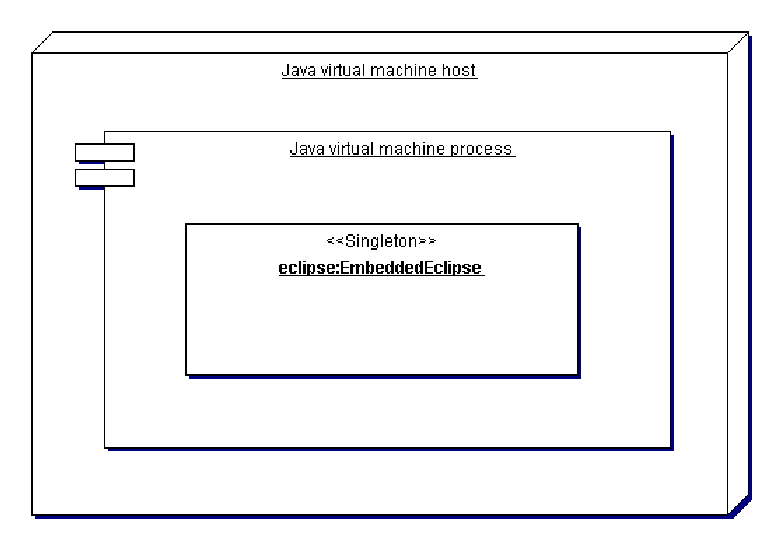
\includegraphics{embjava-diagrams/embedded-deployment.eps}
    \end{center}
    \caption{\label{fig:ji-embedded-deployment}UML deployment diagram for {\it EmbeddedEclipse}}
  \end{figure}
\end{center}



\paragraph{Initialising an {\it EmbeddedEclipse}}

The embedded {\eclipse} which runs within the JVM and shares its
resources, can be started and ended only once during the lifetime of
the JVM. There is no public constructor method for {\it
EmbeddedEclipse}. Initialisation of the embedded {\eclipse} is done
using the static {\tt getInstance} method of class {\it
EmbeddedEclipse} which takes an {\it EclipseEngineOptions} instance as
a parameter. The method uses this to configure and set up {\eclipse}
and then returns an object of type {\it EmbeddedEclipse}. There may
only ever be one instance of {\it EmbeddedEclipse} in a JVM. If the
embedded {\eclipse} has already been set up or if it has been set up
and terminated, subsequent invocations of {\tt getEclipse} with an
{\it EclipseEngineOptions} will throw exceptions. However during the
lifetime of the embedded {\eclipse}, a reference to the unique {\it
EmbeddedEclipse} object can be obtained using the parameterless static
{\tt getEclipse} method.

\paragraph{Termination of an {\it EmbeddedEclipse}}

The {\tt destroy} method which appears in the {\it EmbeddedEclipse}
class will shut the embedded {\eclipse} down. Once the {\tt destroy}
method has been invoked, the invocation of any methods which require
use of the {\eclipse} engine will result in an {\it
EclipseTerminatedException} being thrown. The {\tt destroy} method
should free all the resources of the JVM process which were being used
by the embedded {\eclipse}.

Once the {\it EmbeddedEclipse} has been destroyed, {\tt getEclipse}
can no longer be used during the lifetime of the JVM to initialise an
embedded {\eclipse} engine. In other words, by invoking {\tt destroy},
one removes the ability to use embedded {\eclipse} engines within the
current instance of the JVM.

\subsubsection{Using {\it OutOfProcessEclipse}\index{OutOfProcessEclipse class}}

This section discusses issues specific to the {\it
OutOfProcessEclipse}\index{OutOfProcessEclipse class} class.  With {\it OutOfProcessEclipse}, the
{\eclipse} engine is a child process of the Java virtual
machine. Figure \ref{fig:ji-outOfProcess-deployment} shows this deployment
model in UML notation. The important consequences of this deployment
model are:

\begin{itemize}
\item The {\eclipse} engine uses separate memory and other resources, 
depending on how the operating system allocates these between processes. 
\item Several instances of {\it OutOfProcessEclipse}\index{OutOfProcessEclipse class} can exist in a Java 
virtual machine at any one time.
\item Communication between Java and {\eclipse} is less efficient.
\end{itemize}

\begin{center}
  \begin{figure}[htb] 
  \begin{center} 
    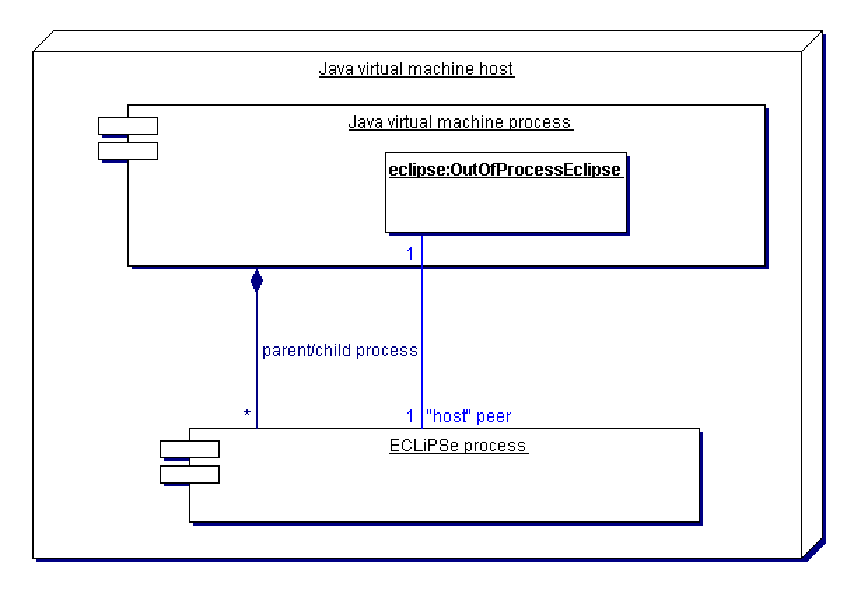
\includegraphics{embjava-diagrams/outOfProcess-deployment.eps}
  \end{center}
  \caption{\label{fig:ji-outOfProcess-deployment}UML deployment
    diagram for {\it OutOfProcessEclipse}} \end{figure}
\end{center}


\paragraph{Initialisation of an {\it OutOfProcessEclipse}\index{OutOfProcessEclipse class}}

{\it OutOfProcessEclipse}\index{OutOfProcessEclipse class} has a single constructor which takes an {\it
EclipseEngineOptions} object as its only parameter. See Section
\ref{sec:ji-eclipse-engine-options} for details of how to create and
configure this object. Unlike {\it EmbeddedEclipse}, multiple {\it
OutOfProcessEclipse}\index{OutOfProcessEclipse class} instances are allowed.

\paragraph{Termination of an {\it OutOfProcessEclipse}}

We invoke the instance method {\tt destroy()} in {\it
OutOfProcessEclipse}\index{OutOfProcessEclipse class} to terminate both the child {\eclipse} process
and our association with it. Once the {\tt destroy} method has been
invoked, the invocation of any methods on the destroyed {\it
OutOfProcessEclipse} object which require use of the {\eclipse} engine will
throw an {\it EclipseTerminatedException}. Unlike {\it
EmbeddedEclipse}, invoking {\tt destroy()} on an {\it
OutOfProcessEclipse} does not affect our ability to create new {\it
OutOfProcessEclipse} instances during the lifetime of the Java virtual
machine.

If the child process {\eclipse} crashes or is killed while {\eclipse}
has control, the Java thread which handed control to {\eclipse} should
throw an {\it EclipseTerminatedException}. If this happens while Java
has control, usually the next invocation of a method on the {\it
OutOfProcesEclipse} should throw an {\it EclipseTerminatedException},
although it is possible that some operations will throw a different
class of {\it IOException}. If this should happen it is worth calling
the {\tt destroy} method to do a final clean-up.

\subsection{Connecting to an existing {\eclipse} engine using {\it RemoteEclipse}\index{RemoteEclipse class}}
\label{sec:ji-connecting-existing}

In some applications, for example where Java is used to visualise
search in {\eclipse}, the life of the {\eclipse} engine may begin
before the connection with Java is initialised or end after the
connection with Java is terminated. Furthermore, it may also be useful
for the eclipse engine and the Java virtual machine to be running on
physically separate computers, for example if the {\eclipse} tasks are
being executed on a compute server, but the Java program is to be run
on a workstation. The {\it RemoteEclipse}\index{RemoteEclipse class} class can be used to connect
Java to {\eclipse} in these two scenarios. The deployment model is
that the {\it RemoteEclipse}\index{RemoteEclipse class} Java object is a ``Proxy'' for the
{\eclipse} engine which is running on the remote machine, as shown in
UML notation in Figure \ref{fig:ji-remote-deployment}.


\begin{center}
  \begin{figure}[htb]
    \begin{center}
        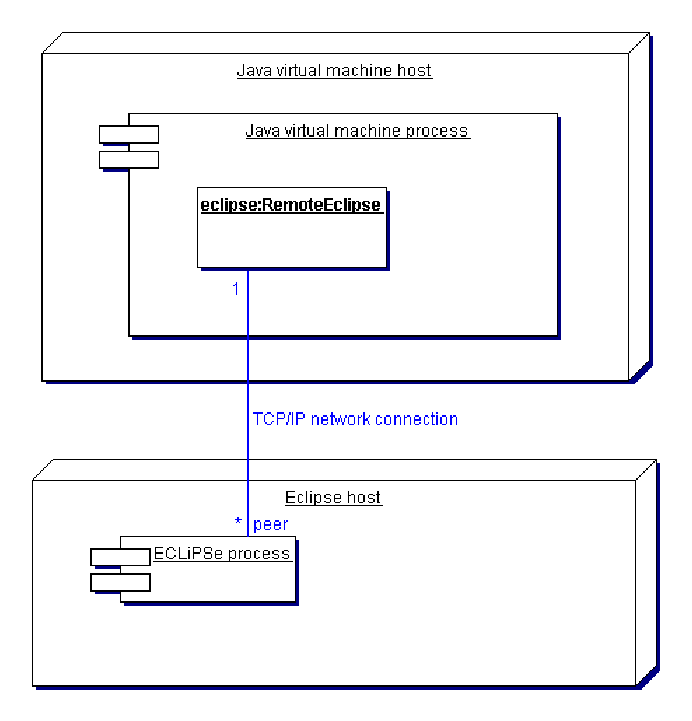
\includegraphics{embjava-diagrams/remote-deployment.eps}
    \end{center}
    \caption{\label{fig:ji-remote-deployment}UML deployment diagram for {\it RemoteEclipse}}
  \end{figure}
\end{center}

The key consequences of this deployment model are:
\begin{itemize}
\item {\eclipse} and Java can run on different machines and the two machines may have a different architecture/OS.  
\item {\eclipse} can connect to multiple Java processes using this model.
\item The lifetime of the {\eclipse} engine need not necessarily be a sub-duration of the lifetime of the JVM. 
\end{itemize}


\subsubsection{Initialisation of a {\it RemoteEclipse}\index{RemoteEclipse class} connection}
\label{sec:ji-remote-init}

Connecting Java to {\eclipse} using {\it RemoteEclipse} requires the
{\eclipse} engine to be primed so that it is ready to accept the
connection.  By the time it connects, the Java program must have the
IP address of the machine hosting the {\eclipse} engine (the server)
and the port number being used for the connection. The attachment
protocol also optionally allows for a password to be used by the Java
side and checked against one specified on the {\eclipse} side. Also
the server must be configured to allow TCP/IP socket servers which can
be connected to by the machine hosting Java. Initialising a connection
using {\it RemoteEclipse}\index{RemoteEclipse class} therefore requires some coordination between
the {\eclipse} code and the Java code. The Java code always consists
of a single {\it RemoteEclipse} constructor invocation, although the
constructor parameters may vary. 

The {\eclipse} side of the code uses certain builtins. Refer to the
relevant documentation of these for precise details of usage. On the
{\eclipse} side, the code can be structured in two different ways; one
simpler and the other allowing more flexibility. We outline here the
sequence of actions in each case.

\paragraph{Basic connection sequence}
This can be used in situations where no password is to be used and
where the port number is specified in advance, rather than generated
dynamically by {\eclipse}, and is known by the Java side.
\begin{enumerate}
  \item The {\eclipse} side executes the builtin \bipref{remote_connect/3}{../bips/kernel/externals/remote_connect-3.html}, specifying the port number in advance. This
	builtin will block until the connection is established.  

  \item The Java side then invokes one of the {\it RemoteEclipse}\index{RemoteEclipse class}
	constructors which has no password parameter. This should
	immediately complete or throw an exception if the connection
	is unsuccessful.

\end{enumerate}
\paragraph{Advanced connection sequence}
This more complicated sequence uses a password and optionally allows
the port number to be generated dynamically and then communicated to
the Java side.
\begin{enumerate}
  \item The {\eclipse} side executes the builtin \bipref{remote_connect_setup/3}{../bips/kernel/externals/remote_connect_setup-3.html}, specifying the password and either
	specifying the port number or allowing it to be generated
	dynamically.

  \item The port number must be communicated to the Java side somehow,
  	e.g. manually, or via a file.

  \item The Java side then invokes one of the {\it RemoteEclipse}\index{RemoteEclipse class}
	constructors with a password parameter. This either blocks
	until the connection is successful or throws an exception.

  \item The {\eclipse} side executes the builtin \bipref{remote_connect_accept/6}{../bips/kernel/externals/remote_connect_accept-6.html}, specifying the password which the
  	Java should supply.

  \item The Java constructor invocation then completes, or throws an
	exception if the connection could not be made.
\end{enumerate}

% something about localhost
If left as a free variable, the {\tt Host} argument of either the \bipref{remote_connect/3}{../bips/kernel/externals/remote_connect-3.html} or \bipref{remote_connect_setup/3}{../bips/kernel/externals/remote_connect_setup-3.html} goal will become
instantiated to the IP address of the machine hosting
{\eclipse}. Another possibility is to call the goal with this argument
already instantiated to the atom {\tt localhost}. This will mean that
only client connections made by processes on the same machine and
using the loopback address will be accepted. With this usage, on the
Java side you should use invoke {\tt
InetAddress.getHostByName("localhost")}. Note that {\tt
InetAddress.getLocalHost()} will not work in this situation.

In both connection sequences, the peer name indexing the connection is
either specified or generated dynamically on the {\eclipse} side in
the \bipref{remote_connect/3}{../bips/kernel/externals/remote_connect-3.html} or \bipref{remote_connect_setup/3}{../bips/kernel/externals/remote_connect_setup-3.html} goal.

Once the connection has been established by one of the above
sequences, control initially rests with the Java side. Therefore the
{\eclipse} code which called the \bipref{remote_connect/3}{../bips/kernel/externals/remote_connect-3.html} goal or the
\bipref{remote_connect_accept/6}{../bips/kernel/externals/remote_connect_accept-6.html} goal blocks until the Java side
explicitly transfers control to {\eclipse} or disconnects.

\subsubsection{Explicit transfer of control between {\eclipse} and Java}
\label{sec:ji-remote-control-transfer}

As mentioned above, after the initial connection has been established,
Java has control by default. However, this may not be convenient. For
example, in the case of search visualisation, after the initialisation
of the visualisation client, we may prefer {\eclipse} to have control
by default, allowing control to pass to Java only on certain
occasions. Control can be explicitly passed from Java to {\eclipse} by
invoking the {\tt resume()} method on a {\it RemoteEclipse}\index{RemoteEclipse class}. In this
case the {\eclipse} code will resume execution after the last point where
it passed control to Java. For example, if {\tt resume()} is invoked
immediately after the {\it RemoteEclipse}\index{RemoteEclipse class} constructor completes,
{\eclipse} execution will resume at the point just after the call to
the \bipref{remote_connect/3}{../bips/kernel/externals/remote_connect-3.html} goal or the \bipref{remote_connect_accept/6}{../bips/kernel/externals/remote_connect_accept-6.html}
goal.

Control can be transferred to a Java peer using the \bipref{remote_yield/1}{../bips/kernel/externals/remote_yield-1.html}
builtin. In this case the Java thread which passed execution to
{\eclipse} will resume execution at the point where it blocked.

The {\tt resume()} method and the \bipref{remote_yield/1}{../bips/kernel/externals/remote_yield-1.html} builtin should be
used with care. An invocation of {\tt resume()} should be paired with
an execution of a \bipref{remote_yield/1}{../bips/kernel/externals/remote_yield-1.html} goal in most cases. In addition,
\bipref{remote_yield/1}{../bips/kernel/externals/remote_yield-1.html} should not be executed in any code executed as a
result of an {\tt rpc}\index{rpc() method} invocation and {\tt resume()} should not be
executed within the {\it QueueListener} methods {\tt dataAvailable()}
or {\tt dataRequest()}.

The {\tt resume()} method and the \bipref{remote_yield/1}{../bips/kernel/externals/remote_yield-1.html} builtin should
only be used when other techniques such as {\tt rpc}\index{rpc() method} are not suitable.

% section not required: the only situation where there are problems can
% never occur, since you cannot read from a closed stream.


% \subsubsection{Using {\it ToEclipseQueue} objects with a {\it RemoteEclipse}}
% \label{sec:ji-toeclipse-remote}
% 
% The {\it java.io} API documentation specifies that the contract of the
% {\tt flush()} method of an {\it OutputStream} is to indicate to the
% stream that, if there are any buffered bytes they should ``immediately
% be written to their destination''. Since {\it ToEclipseQueue} is a
% subclass of {\it OutputStream}, ideally the completion of the {\tt
% flush()} method should guarantee that the bytes have been transferred
% to the {\eclipse} side of the connection. 
% 
% Unfortunately, there is an {\eclipse} limitation preventing this: the
% {\eclipse} side has a limited and fixed buffer size. So, in the case
% of {\it RemoteEclipse}, if a large enough number of bytes are written
% to a {\it ToEclipseQueue} the {\tt flush()} method cannot guarantee
% that the bytes have been transferred. However, it makes a lesser
% guarantee, that the bytes will be transferred as soon as possible when
% space becomes available in the {\eclipse}-side buffer. This will
% happen when a read of the queue is executed on the {\eclipse}
% side. Meanwhile the bytes are buffered on the Java side. When it
% becomes possible, the transfer is done automatically in a separate
% Java thread from the one which invoked {\tt flush}, so the API user
% does not normally need to worry about this.
% 
% The only situation where this potentially causes a problem is where a
% large number of bytes have been written to the {\it ToEclipseQueue}
% which is then flushed and closed before a corresponding read is
% executed on the {\eclipse} side. Since closing the queue does not wait
% for all the bytes to be transferred, these bytes may be lost. This may
% be avoided simply by ensuring that the last {\eclipse}-side read
% occurs before the queue is closed.
%
 
\subsubsection{Termination of a {\it RemoteEclipse} connection}
\label{sec:ji-remote-disconnect}

A {\it RemoteEclipse}\index{RemoteEclipse class} connection between {\eclipse} and Java may be
terminated in different ways. Firstly, disconnection may be initiated
by either side. Secondly the disconnection may be either {\it
multilateral} or {\it unilateral}. Multilateral disconnection, the
preferred method, is where the side which has control initiates
disconnection. Unilateral disconnection is where the side which
initiates disconnection does not have control, and should only take
place as a clean-up routine when one side is forced to terminate the
connection because of an unexpected event.


\begin{description}
 \item[Java-initiated multilateral disconnect] is performed by
 invoking the {\tt disconnect} method on the {\it RemoteEclipse}\index{RemoteEclipse class}
 instance while the Java side has control.

 \item[Java-initiated unilateral disconnect] is performed by
 invoking the {\tt unilateralDisconnect} method on the {\it
 RemoteEclipse}\index{RemoteEclipse class} instance while Java does not have control.

 \item[{\eclipse}-initiated multilateral disconnect] is performed on
 the {\eclipse} side by executing a \bipref{remote_disconnect/1}{../bips/kernel/externals/remote_disconnect-1.html} goal
 while {\eclipse} has control, identifying the connection to be closed
 by supplying the peer name.

 \item[{\eclipse}-initiated unilateral disconnect] cannot be
 executed by the user, since {\eclipse} is not
 multi-threaded. However, it may occur in certain urgent situations
 e.g. if the {\eclipse} process is killed while {\eclipse} does not
 have control.
\end{description}
If an {\eclipse}-initiated disconnect occurs, or the connection is
lost for whatever reason while {\eclipse} has control, the Java thread
which handed control to {\eclipse} should throw an {\it
EclipseTerminatedException}. If either of these happens while Java has
control, the next invocation of a method on the {\it
RemoteEclipse}\index{RemoteEclipse class} should throw an {\it EclipseTerminatedException},
although it is possible that some operations will throw a different
class of {\it IOException}. If this should happen it is worth invoking
the {\tt unilateralDisconnect()} method to do a final clean-up.

\subsection{Comparison of different Java-{\eclipse} connection techniques}
\label{sec:ji-compare-connection-classes}
This section should give you some idea of when it is most appropriate
to use each connection class. Figure \ref{fig:ji-connection-classes}
is a UML class diagram showing the most important relationships and
operations of the principal classes and interfaces. 

All three classes implement {\it EclipseConnection}
\index{EclipseConnection interface}, which provides all the functionality
you would expect during a ``session'' with {\eclipse}. The {\it
EclipseEngine} interface \index{EclipseEngine interface} is implemented
when the JVM ``owns'' the {\eclipse} engine, and so provides the methods to
access the standard I/O streams. Note that the termination methods are not
in either of the interfaces, but are specific to each class. Furthermore,
the {\tt resume()} method allows {\it RemoteEclipse}\index{RemoteEclipse class} to explicitly hand
control to {\eclipse}, but this operation is not supported by the other two
classes.

To summarise the advantages and disadvantages Table
\ref{tab:ji-feature-comparison} gives an at-a-glance comparison of the
different features of the different connection
classes.\index{EclipseConnection interface}\index{EclipseEngine interface}

\begin{center}
  \begin{figure}[htb]
    \begin{center}
        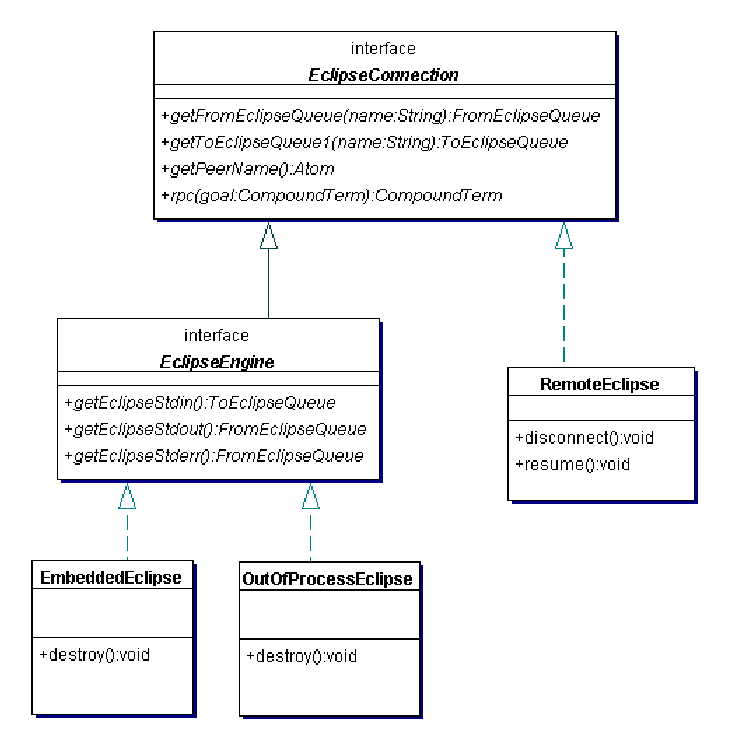
\includegraphics{embjava-diagrams/connection-classes.eps}
    \end{center}
    \caption{\label{fig:ji-connection-classes}UML class diagram for different classes connecting Java and {\eclipse}. Some convenience methods from {\it EclipseConnection} have been omitted.}
  \end{figure}
\end{center}


\begin{table}
\begin{center}
\begin{tabular}{|l|c|c|c|}
\hline
Feature			&\multicolumn{3}{|c|}{Java-{\eclipse} connection class}\\
\cline{2-4}
			&{\it Embedded}&{\it OutOfProcess}	&{\it Remote}\\
\hline
Implements {\it EclipseConnection} interface \ohtml{(allowing {\tt rpc}\index{rpc() method} and queues)}& $\bullet$ & $\bullet$ & $\bullet$\\
\olatex{(allowing {\tt rpc}\index{rpc() method} and queues) & & &\\}
\hline
Implements {\it EclipseEngine} interface \ohtml{(allowing access to {\eclipse} stdio streams)} & $\bullet$ & $\bullet$ & --\\
\olatex{(allowing access to {\eclipse} stdio streams) & & &\\}
\hline
{\eclipse} is in a separate process \ohtml{(with separate memory heap/stack)} & -- & $\bullet$ & $\bullet$ \\
\olatex{(with separate memory heap/stack) & & &\\}
\hline
{\eclipse} can be on a separate \ohtml{machine from Java}  & -- & -- & $\bullet$ \\
\olatex{machine from Java & & &\\}
\hline
{\eclipse} engine can start before/ \ohtml{end after Java virtual machine}  & -- & -- & $\bullet$ \\
\olatex{end after Java virtual machine & & &\\}
\hline
{\eclipse} engine created/ \ohtml{destroyed from Java}  & $\bullet$ & $\bullet$ & -- \\
\olatex{destroyed from Java & & &\\}
\hline
Efficient transfer of data on \ohtml{queues and {\tt rpc} invocations}  & $\bullet$ & -- & -- \\
\olatex{queues and {\tt rpc} invocations & & &\\}
\hline
One {\eclipse} can connect to many \ohtml{Java virtual machines using this}  & -- & -- & $\bullet$ \\
\olatex{Java virtual machines using this & & &\\}
\hline
One Java virtual machine can connect \ohtml{to many {\eclipse} engines using this}  & -- & $\bullet$ & $\bullet$ \\
\olatex{to many {\eclipse} engines using this & & &\\}
\hline
\end{tabular}
\end{center}
\caption{\label{tab:ji-feature-comparison} Feature comparison table for different {\eclipse} connection classes}
\end{table}

%HEVEA\cutend
 



% BEGIN LICENSE BLOCK
% Version: CMPL 1.1
%
% The contents of this file are subject to the Cisco-style Mozilla Public
% License Version 1.1 (the "License"); you may not use this file except
% in compliance with the License.  You may obtain a copy of the License
% at www.eclipse-clp.org/license.
% 
% Software distributed under the License is distributed on an "AS IS"
% basis, WITHOUT WARRANTY OF ANY KIND, either express or implied.  See
% the License for the specific language governing rights and limitations
% under the License. 
% 
% The Original Code is  The ECLiPSe Constraint Logic Programming System. 
% The Initial Developer of the Original Code is  Cisco Systems, Inc. 
% Portions created by the Initial Developer are
% Copyright (C) 2006 Cisco Systems, Inc.  All Rights Reserved.
% 
% Contributor(s): Joachim Schimpf, IC-Parc
% 
% END LICENSE BLOCK
%
% $Id: embexdr.tex,v 1.1 2006/09/23 01:48:59 snovello Exp $
%
% Author:	Joachim Schimpf, IC-Parc
%

%----------------------------------------------------------------------
\chapter{EXDR Data Interchange Format}
\label{chapexdr}
%HEVEA\cutdef[1]{section}
%----------------------------------------------------------------------

We have defined a data interchange format called EXDR for the
communication between {\eclipse} and other languages.  The data types
available in this format are integer, double, string, list, nil,
structure and anonymous variable.  This is intended to be the subset
of {\eclipse} types that has a meaningful mapping to many other
languages' data types.  The mapping onto different languages is given
in the following table. For details of the mapping between Java
classes/interfaces and EXDR/{\eclipse} types see Section
\ref{sec:ji-type-correspondence}.

\begin{quote}
\begin{tabular}{|llll|}
\hline
\bf EXDR type     & \bf ECLiPSe type  &  \bf TCL type  &  \bf Java type\\
\hline
Integer       & integer       &  int	&	java.lang.Integer\\
 e.g.         & 123           &  123	&	123\\
\hline
Long          & integer       &  string	&	java.lang.Long\\
 e.g.         & 5000000000    &  5000000000 &	5000000000\\
\hline
Double        & float         &  double	&	java.lang.Double/Float\\
 e.g.         & 12.3          &  12.3	&	12.3\\
\hline
String        & string        &  string	&	java.lang.String\\
 e.g.         & "abc"         &  abc	&	"abc"\\
\hline
List          & ./2           &  list	&	java.util.Collection\\
 e.g.         & \lbr a,b,c\rbr  &  \{a b c\} &	\\
\hline
Nil           & \nil /0          &  empty string &	java.util.Collection\\
 e.g.         & \nil            &  \{\} "" & \\
\hline
Struct        & compound      &  list	&	CompoundTerm/Atom\\
 e.g.         & foo(bar,3)    &  \{foo bar 3\}&\\
\hline
Variable      & variable      &  string	&	null\\
 e.g.         & _             &  _	&	\\
\hline
\end{tabular}
\end{quote}

The EXDR Integer data type is a 32-bit signed integer, the EXDR Long
data type is a 64-bit signed integer, bigger {\eclipse} integers cannot
be represented.
The EXDR Variable type only allows singleton, anonymous variables,
which means that it is not possible to construct a term where a variable
occurs in several places simultaneously. The main use of these variables
is as placeholders for result arguments in remote procedure calls.


%----------------------------------------------------------------------
\section{{\eclipse} primitives to read/write EXDR terms}
%----------------------------------------------------------------------

The {\eclipse} predicates to create and interpret EXDR-representation
read from and write directly to {\eclipse} streams. This means that
EXDR-format can be used readily to communicate via files, pipes,
sockets, queues etc.
\begin{description}
\item[\biptxtref{write_exdr(+Stream, +Term)}{write_exdr/2}
	{../bips/kernel/ioterm/write_exdr-2.html}]\ \\
    	This predicate writes terms in exdr format.
	The type of the generated EXDR-term is the type resulting
	from the "natural" mapping of the Eclipse terms.
	Atoms are written as structures of arity 0 (not as strings).
	Note that all information about variable sharing, variable
	names and variable attributes is lost in the EXDR representation.

\item[\biptxtref{read_exdr(+Stream, -Term)}{read_exdr/2}
	{../bips/kernel/ioterm/read_exdr-2.html}]\ \\
    	This predicate reads exdr format and constructs a
	corresponding Eclipse term.
\end{description}

Please refer to chapter \ref{chaptcl} for the Tcl primitives,
and to chapter \ref{chapjava} for the Java primitives for manipulating
EXDR terms. 


%----------------------------------------------------------------------
\section{Serialized representation of EXDR terms}
%----------------------------------------------------------------------

The following is the specification of what is actually send over the
communication channels.
This is all the information needed to create new language mappings
for EXDR terms. This definition corresponds to EXDR_VERSION 2:
\begin{quote}\begin{verbatim}
ExdrTerm      ::=   'V' Version CompactFlag? Term
CompactFlag   ::=   'C'
Term          ::=   (Integer|Double|String|List|Nil|Struct|Variable)
Integer       ::=   ('B' <byte> | 'I' XDR_int | 'J' XDR_long)
Double        ::=   'D' XDR_double
String        ::=   ('S' Length <byte>* | 'R' Index)
List          ::=   '[' Term (List|Nil)
Nil           ::=   ']'
Struct        ::=   'F' Arity String Term*
Variable      ::=   '_'
Length        ::=   XDR_nat
Index         ::=   XDR_nat
Arity         ::=   XDR_nat
Version       ::=   <byte>
XDR_int       ::=   <4 bytes, msb first>
XDR_long      ::=   <8 bytes, msb first>
XDR_double    ::=   <8 bytes, ieee double, exponent first>
XDR_nat       ::=   ( <8 bits: 1 + seven bits unsigned value>
                    | XDR_int )                    // >= 0
\end{verbatim}\end{quote}
The version byte is 1 or 2.  EXDR version 1 encodings are also valid
version 2 encodings, and version version 2 decoders can read
version 1 encoded terms.

XDR_long, XDR_int and byte are all signed integers in two's complement
representation.

The string reference code R means that the string is the same as the
Index'th S-encoded string that occurred in the EXDR term earlier.
The presence of the CompactFlag C in the header indicates that the term
may actually contain such string references. If the flag is absent, the
term does not contain any.

%HEVEA\cutend

% BEGIN LICENSE BLOCK
% Version: CMPL 1.1
%
% The contents of this file are subject to the Cisco-style Mozilla Public
% License Version 1.1 (the "License"); you may not use this file except
% in compliance with the License.  You may obtain a copy of the License
% at www.eclipse-clp.org/license.
% 
% Software distributed under the License is distributed on an "AS IS"
% basis, WITHOUT WARRANTY OF ANY KIND, either express or implied.  See
% the License for the specific language governing rights and limitations
% under the License. 
% 
% The Original Code is  The ECLiPSe Constraint Logic Programming System. 
% The Initial Developer of the Original Code is  Cisco Systems, Inc. 
% Portions created by the Initial Developer are
% Copyright (C) 2006 Cisco Systems, Inc.  All Rights Reserved.
% 
% Contributor(s): Kish Shen, IC-Parc
% 
% END LICENSE BLOCK
%
% $Id: embremoteproto.tex,v 1.3 2015/01/14 01:31:09 jschimpf Exp $
%
% Author:       Kish Shen, IC-Parc
%
\chapter{The Remote Interface Protocol}
\label{chapremoteproto}
%HEVEA\cutdef[1]{section}

\section{Introduction}

The {\eclipse} remote interface protocol is used to build a remote
interface between {\eclipse} and some programming language. A program
written in that programming language can interact and communicate with a
separate {\eclipse} process via the remote interface. The Tcl remote
interface (chapter~\ref{chapremote}) is an example of such an
interface. This chapter describes the protocol, so that remote interfaces
to other programming languages can be built.

The protocol is designed to allow the implementer to build an interface
that is compatible with the embedding interface of the same language. This
should allow the same code (in both {\eclipse} and the other language) to
be used in both interfaces. On the {\eclipse} side, the concept of {\it
peers\/} is used to unify the remote and embedding interfaces. 

Another feature of the remote interface is that on the {\eclipse} side,
the interface is independent of the programming language that is being
interfaced to. It should be possible to write {\eclipse} code with the
interface (e.g.\ for a GUI) and change the remote code without needing to
rewrite the code on the {\eclipse} side.

Briefly, a socket connection is established between the remote program and
an {\eclipse} process. The processes exchange messages in the EXDR (see
chapter~\ref{chapexdr}) format according to the protocol. This allows the
communication to be platform independent, and the {\eclipse} and remote
processes can be located on any two machines which can establish socket
connections. 

\section{Basics}
\label{remoteprotobasic}

The remote interface is established by {\bf attaching} the remote and
{\eclipse} processes. The attachment establishes two socket connections
between the two processes:

\begin{description}
\item[Control] This connection is used to control the remote
interface. Messages (in EXDR format) are sent in both directions according
to the remote protocol to co-ordinate the two processes.
\item[Rpc] This is used to send {\bf ec_rpc} goals from the remote process
to {\eclipse} and return the results. The goal is sent in EXDR format.
\end{description}

More than one remote attachment can be established in an {\eclipse}
process. Each attachment is independent, and is a remote peer,
identified by its control
connection. Each remote attachment has two sides: the {\eclipse} side, and
the remote side. 

At any one time, either the {\eclipse} or the remote side has {\it
control}. When a side has control, it is able to send messages to the other
side via the control connection. The side that does not have control
waits for messages to arrive on the control connection. On the {\eclipse}
side, execution is suspended while it does not have control. In general, once a
control message is sent, the control is passed to the other side, and the
side that sent the message waits for a reply message from the other side.

The {\bf ec_rpc} mechanism is designed to be the main way for the remote
side to interact with the {\eclipse} side. The remote side can send an
{\eclipse} goal, in EXDR format to be executed by the {\eclipse} side. This
can only be done while the remote side has control, and when the goal is
issued, a message is sent via the control connection to the {\eclipse}
side, and control is passed to the {\eclipse} side. Control is passed back
to the remote side when {\eclipse} completes the execution of the goal.

After the attachment, extra I/O connections can be established between the
two sides. This allows data to be transferred from one side to the other.
These connections (referred to as peer queues) can be of two types:

\begin{description}
\item[synchronous] These queues are synchronised by the control
connection. Control messages are exchanged between the two sides to ensure
that they are both are synchronised for the data transfer: one side
consumes the data that is sent from the other. This ensures that no
blocking occurs with the I/O operations across the sockets.

\item[asynchronous] These queues can perform I/O operations that are not
 co-ordinated by the control 
connection. Either side can write to or read from the queue 
without transferring control. In fact, if the remote language is
multi-threaded, it can perform asynchronous I/O while {\eclipse}
side has control. Note that asynchronous I/O
operations may block on the {\eclipse} side. 

\end{description}

\section{Attachment}
\label{remoteattach}
\subsection{Attachment Protocol}

\begin{figure}[hbt]
\begin{center}
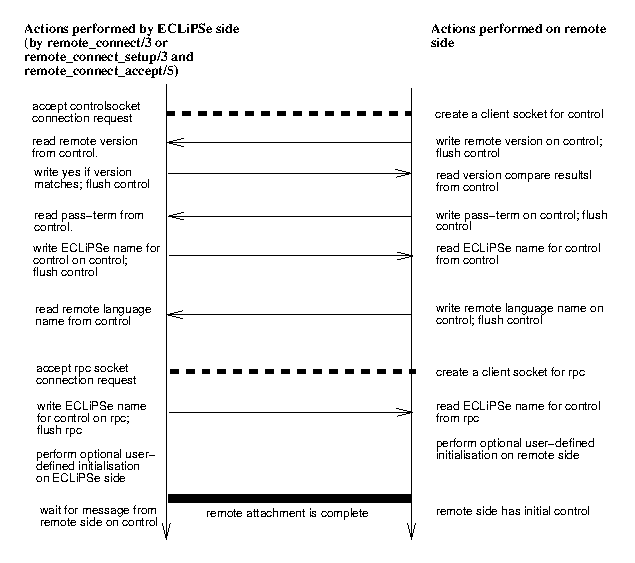
\includegraphics{remoteconnect.ps}
\end{center}
\caption{Summary of the attachment protocol}
\label{rattach}
\end{figure}


The attachment process is summarised in Figure~\ref{remoteattach}. It is
initiated from the {\eclipse} side, by either calling
\bipref{remote_connect/3}{../bips/kernel/externals/remote_connect-3.html} or the more flexible \bipref{remote_connect_setup/3}{../bips/kernel/externals/remote_connect_setup-3.html}
and \bipref{remote_connect_accept/6}{../bips/kernel/externals/remote_connect_accept-6.html} pair. In fact, {\bf remote_connect/3} is implemented using {\bf
remote_connect_setup/3} and {\bf remote_connect_accept/6} with default
values for some of the arguments. 

The attachment can be divided into several phases: 

\begin{enumerate}
\item Initialisation and handshaking: the control connection is
established, and handshaking between the two sides are carried out --
checking that the remote protocols on the two sides are compatible;
checking the pass-term.
\item Establishing the ERPC connections and exchange of information
(remote language, {\eclipse} name for the peer).
\item User-defined initialisations.
\end{enumerate}

The remote protocol version is stored in the flag {\tt
remote_protocol_version}, accessible via \bipref{get_flag/2}{../bips/kernel/env/get_flag-2.html}
as an integer version number.
This version number should only change when the protocol is
modified. Checking of the version ensures that the same (or at
least compatible) versions of the protocol are used, so that the two sides
behaves correctly. The version information is sent from the remote side
(which must have its own copy of the version information), and the
{\eclipse} side checks that this is compatible with the protocol version it
is using. In order to cope with remote connections which may not be using
the remote protocol, the {\eclipse} side waits only for a fixed period of
time for the remote side to send the version information before timing out.

Time-out on the {\eclipse} side can also occur for forming any of the
connections between the two sides, from the control connection to the peer
queue. This is specified by the user in {\tt remote_connect_accept/6}. If
time-out occurs during the attachment, then the attachment process is
abandoned, and the predicate fails (any connected sockets will be closed).

The detailed sequence of events for the attachment for the remote side
(with some description of the relevant {\eclipse} side actions) are:

\begin{enumerate}
\item {\eclipse} side: a socket server for the control connection is
created, using the address Host/Port which can be specified by the
user. It then waits to accept a socket stream for the control connection
from the remote side. The user can specify the amount of time to wait
before this operation times-out, which would then terminate the attachment.

\item Remote side: create a client socket stream for the control connection,
with an address compatible with Host/Port. The socket stream should
be in blocking mode, and perform no translation on the data sent.
\item Remote side: sends the remote protocol version information on the
control socket in EXDR format and flush it. This should be a {\tt
remote_protocol/1} term. 
\item {\eclipse} side: reads the EXDR version term from the control
socket, and compares with the version on the {\eclipse} side. If the two
protocols are compatible, it sends the EXDR string {\tt yes} back to
the remote side; otherwise it sends the {\eclipse} remote protocol version
to the remote side and disconnects from the remote side (raising
unimplemented functionality error). The {\eclipse} side waits at
most 100 seconds after the control connection is established for the remote side's version: after
this the {\eclipse} side disconnects the control connection and raises out
of range error. 
\item It is expected that the future versions of the protocol will remain
unchanged up to this point at least, to ensure the proper handshaking and
checking of versions.
\item Remote side: write the `pass-term' in EXDR format on the newly created control
connection and flush it. This provides a simple security check: {\eclipse}
side will check if the `pass-term' matches the `pass-term' it was given
when the remote connection was initiated -- for \bipref{remote_connect/3}{../bips/kernel/externals/remote_connect-3.html}, the
pass-term is the empty string, but the user can specify any pass-term if
\bipref{remote_connect_setup/3}{../bips/kernel/externals/remote_connect_setup-3.html} and \bipref{remote_connect_accept/6}{../bips/kernel/externals/remote_connect_accept-6.html} are
used. If the terms are not identical, then the {\eclipse} side will
discontinue the attachment process.

\item Remote side: read from the control connection the {\eclipse} name for the control
connection. This is sent in EXDR format, and is used to identify this
particular remote attachment -- the peer name for the peer. This name is needed when calling ec_rpc goals
that refer to the peer. 
\item Remote side: write the name of the programming language (e.g.\ tcl, java) of the
remote process on the control connection. This should be in EXDR string
format, and the connection flushed. 
\item {\eclipse} side: read the name of the programming language and store
it (it can be accessed later via \bipref{peer_get_property/3}{../bips/kernel/externals/peer_get_property-3.html}). The {\eclipse}
side now wait to accept the socket stream (using the same socket server as
the control connection) for the ec_rpc connection. This can also time-out.
\item Remote side: create a client socket stream for the ec_rpc connection, using the
same Port as for the control connection. This stream should be in
blocking mode, and perform no translation on the data sent. The server
socket on the {\eclipse} will be closed after accepting this client.
\item Remote side: read the control connection name again on the remote side, on the
newly established ec_rpc connection. This is also sent in EXDR format. This
is designed to verify that the ec_rpc connection is indeed connected to the
{\eclipse} side. 
\item Remote side: the remote side now has control. Any user-defined initialisations on the remote
side can now be performed, to make the remote side ready for the
interaction. The remote side has the control initially. Note that
user-defined initialisations on the {\eclipse} side is also performed after
sending the control name on the ec_rpc connection. After the
initialisation, {\eclipse} side will suspend and listen on the control
connection for the remote side to give control back to the {\eclipse} side.
\end{enumerate}

At the end of this, the remote side should be ready for normal interaction
with the {\eclipse} side.

The remote_connect/3 or remote_connect_accept/6 predicate waits for the control to be handed back by
the remote side before exiting. Thus when the predicate succeeds, the
remote side has been attached and properly initialised, with {\eclipse}
side having control.

The protocol does not specify how the remote side should be informed of the
Host/Port address for the initial socket connection. The Address can be
fixed before hand (with the Address argument instantiated, or
the information can be transmitted either manually or via files. In
addition, the remote process can be started from within {\eclipse} using
the \bipref{exec/3}{../bips/kernel/opsys/exec-3.html} command, with the host and port supplied as arguments.

In accepting client socket connections from the remote side, the {\eclipse}
side is informed of the host of the remote side. This should either be the
client's hostname, or 'localhost'. After accepting the control connection,
subsequent connections (for ec_rpc and any peer queues) are checked to
ensure that they are from the same client. If not, the attachment is
terminated by {\eclipse}. Using 'localhost' as the name on either side will
restrict the two sides to be on the same machine (and they must both use
localhost for Host in the address, rather than the actual hostname). 

\subsection{An example}

The following is a simple example of making a remote attachment on the
remote side. In this case, the remote side is also an {\eclipse} program.
A remote attachment by a program written in another programming language
will need to provide a similar function in that language:

\begin{verbatim}
% Example code for making a remote attachment on the remote side

:- local variable(ecsidehost).

% remote_attach/6 makes a remote attachment to a host ECLiPSe program.
% Args:
%    +Host: host name on ECLiPSe side
%    +Port: port on ECLiPSe side
%    +Pass: `pass-term' - used to verify the connection
%    +Init: goal to call to perform any application specific initialisation
%    -Control: the remote side (local) name of the control connection
%    -Ec_rpc:  the remote side name of the ec_rpc connection
%    -EcSideControl: the ECLiPSe side name for the control connection

remote_attach(Host, Port, Pass, Init, Control, Ec_rpc, EcSideControl) :-
     % control connection
     new_client_socket(Host, Port, Control),
     % send the protocol version information to the ECLiPSe side
     % we are the remote side, so must have our own version info.
     write_exdr(Control, remote_protocol(1)), flush(Control),
     % read response from ECLiPSe side to make sure it is compatible...
     read_exdr(Control, IsSameVersion),
     (IsSameVersion == "yes" ->
         true 
     ; 
         writeln("Incompatible versions of remote protocol. Failing...."),
         fail
     ),
     % send pass-term; if this does not match the pass-term on the ECLiPSe
     % side, it will terminate the attachment
     write_exdr(Control, Pass), flush(Control),
     % ECLiPSe side name for connection
     read_exdr(Control, EcSideControl),
     % send language name to ECLiPSe side
     write_exdr(Control, "eclipse"), flush(Control),
     % Ec_rpc connection
     new_client_socket(Host, Port, Ec_rpc),
     % read control name again on Ec_rpc to verify connection
     % in a more sophisticated implementation, this should time-out
     (read_exdr(Ec_rpc, EcSideControl) ->
        true 
     ; 
	% if not verified, terminate connection
        close(Control), close(Ec_rpc),
        fail
     ),
     % Remote side now has control, call Init to perform application
     % specific initialisations
     call(Init),
     % hand control over to ECLiPSe side...
     write_exdr(Control, resume), flush(Control).


new_client_socket(Host, Port, Socket) :-
     socket(internet, stream, Socket),
     connect(Socket, Host/Port).

%----------------------------------------------------
% the following code make use of remote_attach/6 to make an attachment,
% and then disconnect immediately when ECLiPSe side returns control

test(Host, Port) :-
     % make the remote attachment. For this simple example, there is no
     % application specific initialisations, and the default pass-term
     % of an empty string is used...
     remote_attach(Host, Port, "", true, Control, Ec_rpc, _),
     % control has been given to ECLiPSe side,
     % wait for ECLiPSe side to return control....
     read_exdr(Control, _),
     % immediately disconnect from ECLiPSe side
     write_exdr(Control, disconnect), flush(Control),
     % wait for ECLiPSe side to acknowledge disconnect...
     read_exdr(Control, disconnect_yield),
     % clean up
     close(Control), close(Ec_rpc).

\end{verbatim}

In addition to the attachment, the example contains a very simple example
of using the protocol by exchanging control messages with the {\eclipse}
side. After attachment, it disconnects the remote attachment as soon as
control is handed back to it. For more details on the messages, see next
section. 

To try out the example, start an {\eclipse} session and initiate a remote
attachment. This process is the {\eclipse} side:

\begin{verbatim}
(ECLiPSe side)
[eclipse 1]: remote_connect(Host/Port, Control, _).
Socket created at address chicken.icparc.ic.ac.uk/32436
\end{verbatim}

Now start another {\eclipse} session, compile the example program, and make
the attachment to the {\eclipse} side:

\begin{verbatim}
(Remote side)
[eclipse 4]: test('chicken.icparc.ic.ac.uk', 32436).
\end{verbatim}

On the {\eclipse} side, {\tt remote_connect/3} should now succeed:

\begin{verbatim}
(ECLiPSe side)
Host = 'chicken.icparc.ic.ac.uk'
Port = 32436
Control = peer3
yes.
[eclipse 2]: 
\end{verbatim}

The remote side is suspended, awaiting the {\eclipse} side to return
control. To return control to the remote side, the {\eclipse} side should
call \bipref{remote_yield/1}{../bips/kernel/externals/remote_yield-1.html} (see section~\ref{remotesupport} for a description
of {\tt remote_yield/1}):

\begin{verbatim}
(ECLiPSe side)
[eclipse 2]: remote_yield(peer3).
Abort
[eclipse 3]:
\end{verbatim}

In this simple example, when control is returned to remote side, it
immediately disconnects, thus the {\tt remote_yield/1} on the {\eclipse}
side is aborted (as disconnect was initiated from the remote side), as per
the disconnect protocol.

\begin{verbatim}
(Remote side)
[eclipse 4]: test('chicken.icparc.ic.ac.uk', 32436).

yes.
[eclipse 5]: 
\end{verbatim}

\section{Remote Peer Queues}

As discussed in section~\ref{remoteprotobasic}, peer queues can be formed
interactively during an attachment between the two sides. The protocol
provides for the creation and closing of these queues on both sides. 

The handling of data on these queues are performed by {\it data handlers},
routines which either provide data to the queue or consume data from the
queue. They are triggered by the appropriate control messages, so that a
data consumer handler would consume data arriving on a queue, and a data
provider handler would send data onto a queue (which would be consumed on
the other side). These data handlers can be user defined. 

The programmer for the remote side needs to provide the remote side of the
interface to the peer queue. 

\subsection{Synchronous peer queues}

The implementation of a synchronous peer queue on the {\eclipse} side is
shown in figure~\ref{syncpeer}. There is an in-memory buffer, which is
\begin{figure}[hbt]
\begin{center}
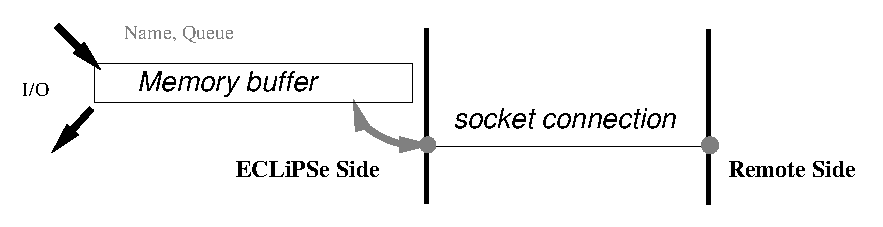
\includegraphics{syncpeer.ps}
\end{center}
\caption{{\eclipse} implementation of remote synchronous peer queue}
\label{syncpeer}
\end{figure}
implemented as a memory queue in {\eclipse} (i.e. {\tt queue("")} option
for \bipref{open/3}{../bips/kernel/iostream/open-3.html}). Associated with the memory queue is the actual socket
stream to the remote side.
The memory queue is the queue that the user sees on the {\eclipse}
side, with name {\it Name} and a unique integer id {\it Queue}, which is
the stream id for the memory queue. The id is used by both sides to identify
the queue, as it is unique (a symbolic name can always be reassigned), and
is used in the control messages. To conform to normal {\eclipse} streams,
these queues appear uni-directional to the user, i.e. data can be either
written to or read from the queue. The direction is {\it fromec} if the
direction of the data is from {\eclipse} to the remote side (i.e.\ 
{\eclipse} can output to the queue), and {\it toec}
if the direction is from the remote side to {\eclipse} (i.e.\ {\eclipse}
can read from the queue). The user perform normal I/O operations on the
memory queue, and the protocol ensures that the data is transferred
correctly to the remote side without blocking.

The socket stream is largely hidden from the user on the {\eclipse} side,
with data automatically transferred between it and the buffer. The buffer
is needed to ensure that when data is transferred between the two sides,
the I/O operation is synchronised (the data is being read on one end of the
socket while it is being written at the other), so no blocking will occur.
When a side needs to initiate an I/O operation with the other side (either
to write data to or read data from the other side via the socket stream), it must have control
(otherwise it would not be in a position to initiate an action). Before
performing the I/O operation, a control message is sent to the other side to
allow it to prepare to read the data before the I/O operation is actually
initiated. The memory queue thus serves to buffer the data before it is
transferred to the socket stream.

The socket stream must be connected to the remote side before it could be
used. Control messages are used also to synchronise the connection of
the socket. The protocol does not specify if a buffer is needed on the
remote side, this depends on the facilities available in the language used
for the remote side.

For a particular synchronous queue, a data handler can only be defined on
one side of the queue, but not both.
 
\subsection{Asynchronous peer queues}

I/O operations on these queues do not need to be controlled by the remote
protocol, but their creation and closing is controlled by the remote
protocol, so that the remote interface can keep track of these queues.
These are implemented as raw socket streams on the {\eclipse}
side, with I/O operations performed directly on the socket. The Name and
Queue id for the stream is thus those for the {\eclipse} socket stream. It
is the responsibility of the user to ensure that I/O operations do not
block on these queues. They are provided to allow asynchronous transfer of
data (e.g.\ from {\eclipse} side to the remote side without handing over
control), and also they allow more efficient transfer of data.  

\section{Control Messages}

These are the messages that are exchanged between the {\eclipse} and remote
sides when the remote side is attached. The messages are sent on the
control connection, and are in EXDR format. All arguments for the messages
are either atoms or integers. The messages are used to
co-ordinate and synchronise the two sides. A message should only be sent from a
particular side when that side has control, and control is handed over
to the other side when the message is sent. 

Most messages are used to initiate an {\it interaction\/} with the
other side. That is, used to cause some action to take place on the
other side: control is handed over, the action takes place on the other
side, and eventually control is handed back 
when the action is completed. Control can also be explicitly handed over
from one side to the other so that the other side can initiate
interactions. Some additional messages can only be sent as part of an
interaction, for exchanges of information between the two sides. Finally,
there are messages for terminating the remote attachment. Note that
interactions can be nested, that is, an interaction from one side can
contain an interaction initiated from the other side. 

The implementer for the remote interface should provide the methods for a
programmer to initiate the interactions from the remote side. These
routines would send the appropriate control messages to the {\eclipse}
side, and the messages should not be directly visible to the programmer. 

The usage of each message is summarised in the diagram(s) accompanying
them. These diagrams show:

\begin{itemize}
\item time proceeds downward. The {\eclipse} side is shown on the left,
the remote side on the right. Messages are shown as vertical arrows between
the two sides. The direction of the arrow indicates the direction the
message is sent.

\item the context in which the message can be sent, i.e.\ the message from
the other side that it is either expecting as a response, or that it is a
response to. The message sequence is shown, with the message highlighted.

\item any accompanying actions expected with the message. These actions are
either sending or receiving data on some other connections between the two
sides. These are shown as dashed arrows in the diagrams.

\item whether nested interactions can take place between messages of an interaction.
This is indicated by vertical ellipsis between the messages in
the diagram. In such cases, the nested interaction can be initiated, and this
interaction completed before the next message for the original interaction
is expected.
\end{itemize}

\subsection{Messages from {\eclipse} side to remote side}

 
\begin{description}
\item[yield] this yields control to the remote side.  The message is used either to
implicitly return control to the remote side at the end of an 
interaction initiated from the remote side, or it
is used to explicitly hand over control to the remote side. 


\begin{center}
% use toimage to generate images for hevea - _ needs to be \_
\begin{toimage}
\begin{picture}(200,70)
\thicklines
\put(70,52){\bf yield}
\put(20,50){\vector(1,0){150}}
\put(0,65){ECLiPSe}
\put(150,65){Remote}
\put(70,25){\shortstack{.\\.\\.\\.\\.\\.}}
\put(20,0){\line(0,1){65}}
\put(170,0){\line(0,1){65}}
\end{picture}
\begin{picture}(200,70)
\put(40,52){rpc {\footnotesize \it (goal via rpc)}}
\put(170,50){\vector(-1,0){150}}
\put(20,46){\dashbox{5}(150,0){}}
\put(20,46){\vector(-1,0){0}}
\put(20,10){\dashbox{5}(150,0){}}
\put(170,10){\vector(1,0){0}}
\thicklines
\put(40,16){{\bf yield} {\footnotesize \it (answer via rpc)}}
\put(20,14){\vector(1,0){150}}
\put(0,65){ECLiPSe}
\put(150,65){Remote}
\put(40,25){\shortstack{.\\.\\.\\.}}
\put(20,0){\line(0,1){65}}
\put(170,0){\line(0,1){65}}
\put(40,0){\shortstack{.\\.}}
\end{picture}
\begin{picture}(210,80)
\thicklines
\put(40,12){{\bf yield}}
\put(20,10){\vector(1,0){170}}
\thinlines
\put(20,46){\dashbox{5}(170,0){}}
\put(20,46){\vector(-1,0){0}}
\put(40,52){{\bf rem\_flushio(Q)} {\footnotesize \it (data via Q)}}
\put(190,50){\vector(-1,0){170}}
\put(0,65){ECLiPSe}
\put(170,65){Remote}
\put(40,25){\shortstack{.\\.\\.\\.}}
\put(20,0){\line(0,1){65}}
\put(190,0){\line(0,1){65}}
\put(40,0){\shortstack{.\\.}}
\end{picture}
\begin{picture}(210,80)
\thicklines
\put(40,12){{\bf yield}}
\put(20,10){\vector(1,0){170}}
\thinlines
\put(20,46){\dashbox{5}(170,0){}}
\put(20,46){\vector(-1,0){0}}
\put(30,52){{\bf rem\_flushio(Q,L)} {\footnotesize \it (L bytes via Q)}}
\put(190,50){\vector(-1,0){170}}
\put(0,65){ECLiPSe}
\put(170,65){Remote}
\put(40,25){\shortstack{.\\.\\.\\.}}
\put(20,0){\line(0,1){65}}
\put(190,0){\line(0,1){65}}
\put(40,0){\shortstack{.\\.}}
\end{picture}
\begin{picture}(210,60)
\put(40,32){queue\_close(Q)}
\put(170,30){\vector(-1,0){150}}
\thicklines
\put(40,12){\bf yield}
\put(20,10){\vector(1,0){150}}
\put(0,45){ECLiPSe}
\put(150,45){Remote}
\put(20,0){\line(0,1){45}}
\put(170,0){\line(0,1){45}}
\put(40,0){\shortstack{.\\.}}
\end{picture}
\begin{picture}(200,120)
\put(40,92){queue\_create(N,T,D,E)}
\put(170,90){\vector(-1,0){150}}
\put(40,77){socket\_client(P,N,T,D)}
\put(20,75){\vector(1,0){150}}
\put(40,62){socket\_connect(N,S)}
\put(170,60){\vector(-1,0){150}}
\put(40,47){socket\_accept(N,Q)}
\put(20,45){\vector(1,0){150}}
\put(40,32){resume}
\put(170,30){\vector(-1,0){150}}
\put(40,20){\shortstack{.\\.\\.}}
\thicklines
\put(40,12){{\bf yield}}
\put(20,10){\vector(1,0){150}}
\put(0,108){ECLiPSe}
\put(150,108){Remote}
\put(20,0){\line(0,1){105}}
\put(170,0){\line(0,1){105}}
\put(40,0){\shortstack{.\\.}}
\end{picture}
\end{toimage}
\imageflush
\end{center}

The interaction-initiating messages from the remote side will be described
in more detail in their own sections.

\item[ec_flushio(Queue, Length)] this message is sent when output on a remote
synchronous queue is flushed on the {\eclipse} side:

\begin{center}
\begin{toimage}
\begin{picture}(200,70)
\put(40,12){resume}
\put(190,10){\vector(-1,0){170}}
\put(20,46){\dashbox{5}(170,0){}}
\put(190,46){\vector(1,0){0}}
\thicklines
\put(40,52){{\bf ec\_flushio(Q,L)} {\footnotesize \it (L bytes via Q)}}
\put(20,50){\vector(1,0){170}}
\put(0,65){ECLiPSe}
\put(170,65){Remote}
\put(40,25){\shortstack{.\\.\\.\\.}}
\put(20,0){\line(0,1){65}}
\put(190,0){\line(0,1){65}}
\put(40,0){\shortstack{.\\.}}
\end{picture}
\end{toimage}
\imageflush
\end{center}

Queue is the
{\eclipse} stream number for the peer queue, and Length is the number of bytes
that is being sent on the queue. Control is yielded to the remote
side. The data on the queue Queue will be sent through the
queue after sending this message on the control connection, so on receiving
this message on the remote side, the remote side should read Length bytes from
Queue. After processing the data, the remote side should return
control to the {\eclipse} side via a {\bf resume} message.

\item[ec_waitio(Queue)] this message is sent when {\eclipse} requests input
from a remote synchronous queue, and the data is not available in the
queue's buffer. 

\begin{center}
\begin{toimage}
\begin{picture}(210,100)
\put(30,12){resume}
\put(190,10){\vector(-1,0){170}}
\put(30,32){yield}
\put(20,30){\vector(1,0){170}}
\put(20,56){\dashbox{5}(170,0){}}
\put(20,56){\vector(-1,0){0}}
\put(30,62){rem\_flushio(Q,L) {\footnotesize \it (L bytes via Q)}}
\put(190,60){\vector(-1,0){170}}
\thicklines
\put(30,82){{\bf ec\_waitio(Q)}}
\put(20,80){\vector(1,0){170}}
\put(0,95){ECLiPSe}
\put(170,95){Remote}
\put(20,0){\line(0,1){95}}
\put(190,0){\line(0,1){95}}
\put(30,70){\shortstack{.\\.}}
\put(30,40){\shortstack{.\\.\\.}}
\put(30,20){\shortstack{.\\.}}
\put(30,0){\shortstack{.\\.}}
\end{picture}
\begin{picture}(210,100)
\put(30,12){resume}
\put(190,10){\vector(-1,0){170}}
\put(30,32){yield}
\put(20,30){\vector(1,0){170}}
\put(20,56){\dashbox{5}(170,0){}}
\put(20,56){\vector(-1,0){0}}
\put(30,62){rem\_flushio(Q) {\footnotesize \it (data via Q)}}
\put(190,60){\vector(-1,0){170}}
\thicklines
\put(30,82){{\bf ec\_waitio(Q)}}
\put(20,80){\vector(1,0){170}}
\put(0,95){ECLiPSe}
\put(170,95){Remote}
\put(20,0){\line(0,1){95}}
\put(190,0){\line(0,1){95}}
\put(30,70){\shortstack{.\\.}}
\put(30,40){\shortstack{.\\.\\.}}
\put(30,20){\shortstack{.\\.}}
\put(30,0){\shortstack{.\\.}}
\end{picture}
\end{toimage}
\imageflush
\end{center}

This interaction is triggered when the {\eclipse} side attempts a read
operation on the empty buffer of a peer queue. The operation is suspended, 
and control is yielded to remote side so that it can provide
the required data. There should be a data-provider handler associated with
the queue on the remote side. This handler should obtain the data, and send
the data to the {\eclipse} side. The data will arrive from the remote side via a
{\bf rem_flushio} message, which initiates a remote flushio interaction, nested
within the {\eclipse} waitio interaction. The data arrives on the socket
associated with the remote peer queue Queue, and is automatically copied by
{\eclipse} into the peer queue buffer. Control is then yielded back to 
the remote side, completing the flushio interaction. The remote side then
hands control back to {\eclipse} side by the resume message. The suspended
read operation is resumed on the now non-empty buffer. 

The remote flushio interaction is described in more detail in its own
section. The main difference between a remote flushio initiated on the
remote side and one initiated by an {\eclipse} waitio described here is
that there must not be a data-consumer handler on the {\eclipse} side, as
the data is to be consumed by the suspended read operation instead.
This is ensured in the protocol by prohibiting handlers on both sides 
of a synchronous peer queue.

Note that the {\eclipse} side will also listen to the control connection
while waiting for the data to be sent from the remote side. If a {\bf
resume} is sent before the data arrives, this is likely caused by a
programming error in the data provider handler, which finished without
sending data to the {\eclipse} side. The {\eclipse} side will print a
warning message on the warning output stream, and immediately yield
back to the remote side. Other messages are handled as normal, recursively
while waiting for the data to arrive -- this is mainly intended to allow
for unexpected aborts from the remote side, although it could also be used to
perform ec_rpc calls before the remote side sends the data.

\item[socket_client(Port, Name, Type, Dir)] this requests the remote side
to form a client socket connection for the remote peer queue Name. The
queue is of type Type (sync or async), and direction Dir (fromec, toec for
synchronous queues, bidirect for asynchronous queues). The client socket is
to connect at port Port with the {\eclipse} side host name.  

\begin{center}
\begin{toimage}
\begin{picture}(200,100)
\put(40,52){socket\_connect(N,S)}
\put(170,50){\vector(-1,0){150}}
\put(40,37){socket\_accept(N,Q)}
\put(20,35){\vector(1,0){150}}
\put(40,12){resume}
\put(170,10){\vector(-1,0){150}}
\put(40,15){\shortstack{.\\.\\.}}
\put(40,0){\shortstack{.\\.\\.}}
\thicklines
\put(40,67){{\bf socket\_client(P,N,T,D)}}
\put(20,65){\vector(1,0){150}}
\put(0,88){ECLiPSe}
\put(150,88){Remote}
\put(20,0){\line(0,1){85}}
\put(170,0){\line(0,1){85}}
\end{picture}
\end{toimage}
\imageflush
\end{center}

The {\eclipse} side first creates a server socket for the peer queue Name.
The port address is Port. This, along with the details of the queue is
passed to the remote side via the {\bf socket_client} message. The remote side
should then connect a client socket with Port as the port, and the Host
used for the initial attachment (which is either localhost or the hostname
of the \verb'eclipse' side) for the host. 
It should also perform any additional
setups for the peer queue using the information sent with the message
(typically this involves setting up book-keeping information for the queue
on the remote side). When the remote side connection is established, it
returns control to {\eclipse} via a {\bf socket_connect} message:

\noindent
{\bf socket_connect(Name, Status)}

Name is the name of the queue, and should be the same as the Name sent by
the socket_client message. This is used to verify that the messages refer
to same interaction. The {\eclipse} side will raise an error and disconnect
from the remote side if the name does not match. Status is either 
success or fail, depending on if the remote side successfully created the
remote side of the queue or not.

If Status is success, then the {\eclipse} side will complete the connection
for the peer queue by accepting the socket connection. Since the remote end
of the socket exists, the accept operation should succeed very
quickly. If not, the operation will time-out, using the time-out interval
specified when the attachment was made. The server socket is closed
immediately after the accept operation. On successful connection,
{\eclipse} first checks that this client's host is indeed the same as the
one previously recorded for the remote side. If so, the
{\eclipse} will finish creating the {\eclipse} side of the queue. If not,
the connection is closed, and the operation is considered to have failed. 

If Status from the socket_connect message is fail,
then the {\eclipse} side will clean up the preparation for the peer queue. 

The {\eclipse} side then returns control to the remote side via a
{\bf socket_accept} message:

\noindent
{\bf socket_accept(Name,Queue)}

Name is again the name of the queue, and Queue the stream id. If the accept
was unsuccessful (or if Status for socket_connect was fail), then Queue
will be the atom fail, indicating that the peer queue connection was
unsuccessful. 

The remote side should then record the  id Queue for later use (it is
needed for the control messages connected with this peer queue). If instead
fail was received, then the remote side should clean up the attempted queue
connection. When the remote side has finished the final stage of the
connection, control is returned to the {\eclipse} side via a {\bf resume}
message, and the socket_client interaction completes.

Note that the {\bf socket_connect} and {\bf socket_accept} messages are
always exchanged during a socket_client interaction, even if the connection
failed on the remote side before {\bf socket_connect} is sent. They also
can only occur in this context. If these messages occur in any other
occasion, an error should be raised.

\item[queue_close(Queue)] this message is sent when the {\eclipse} side
closes the peer queue with id Queue. 

\begin{center}
\begin{toimage}
\begin{picture}(200,60)
\put(40,12){resume}
\put(170,10){\vector(-1,0){150}}
\thicklines
\put(40,32){{\bf queue\_close(Q)}}
\put(20,30){\vector(1,0){150}}
\put(0,45){ECLiPSe}
\put(150,45){Remote}
\put(20,0){\line(0,1){45}}
\put(170,0){\line(0,1){45}}
\put(40,0){\shortstack{.\\.}}
\end{picture}
\end{toimage}
\imageflush
\end{center}

The remote side should close the remote side of the peer queue Queue, and
remove all bookkeeping information associated with it. Control should then
be returned to {\eclipse} via a {\bf resume} message. The {\eclipse} side should
also close the queue and remove bookkeeping information on the {\eclipse} side.

\item[disconnect] this message is sent when {\eclipse} side initiates
disconnect. 

\begin{center}
\begin{toimage}
\begin{picture}(200,60)
\put(70,12){disconnect\_resume}
\put(170,10){\vector(-1,0){150}}
\thicklines
\put(70,32){\bf disconnect}
\put(20,30){\vector(1,0){150}}
\put(0,45){ECLiPSe}
\put(150,45){Remote}
\put(20,10){\line(0,1){35}}
\put(170,10){\line(0,1){35}}
\end{picture}
\end{toimage}
\imageflush
\end{center}

Control is yielded to the remote side, which should acknowledge
with the {\bf disconnect_resume} message. Once the {\eclipse} side receives this
message, the connection between the two sides is considered
terminated. The {\eclipse} side will then close all the connections (the
control and ec_rpc connections, and any asynchronous and synchronous
queues) to the remote side, and clean up the information associated with the
attachment. After sending the disconnect_resume message, the remote side
should also shutdown its end of the connection by closing all the
connections on its side. 

Note that the disconnection message can be used to terminate the attachment
from within an interaction. In such cases, the interaction(s) would not be
completed.

\item[disconnect_yield] this message is sent when {\eclipse} side receives
a {\bf disconnect} message from the remote side, i.e.\ the remote side
initiated disconnection. 

\begin{center}
\begin{toimage}
\begin{picture}(200,60)
\put(50,32){disconnect}
\put(170,30){\vector(-1,0){150}}
\thicklines
\put(50,12){\bf disconnect\_yield}
\put(20,10){\vector(1,0){150}}
\put(0,45){ECLiPSe}
\put(150,45){Remote}
\put(20,10){\line(0,1){35}}
\put(170,10){\line(0,1){35}}
\end{picture}
\end{toimage}
\imageflush
\end{center}

This message is sent as an acknowledgement to the
disconnect message. Once the disconnect_yield is sent, the connection is
considered terminated, and the {\eclipse} side will close all the
connections and clean up. After the clean up, abort is called. This is
done because the application on the {\eclipse} side (such as the remote
development tools) may be deep inside some interaction loop with the remote
side, and abort is the most general way of escaping from such a loop. It
can be caught (see \bipref{remote_yield/1}{../bips/kernel/externals/remote_yield-1.html} in section~\ref{remotesupport}) if
the user wants a more graceful termination. 


\end{description}

\subsection{Messages from remote side to {\eclipse} side}


\begin{description}

\item[resume] this message hands over control from remote side to
{\eclipse} side. This is used to either implicitly return control to the
{\eclipse} side at the end of an interaction initiated from the {\eclipse}
side, or to explicitly hand over control to the remote side.

\begin{center}
\begin{toimage}
\begin{picture}(200,70)
\thicklines
\put(70,52){\bf resume}
\put(170,50){\vector(-1,0){150}}
\put(0,65){ECLiPSe}
\put(150,65){Remote}
\put(70,25){\shortstack{.\\.\\.\\.\\.\\.}}
\put(20,0){\line(0,1){65}}
\put(170,0){\line(0,1){65}}
\end{picture}
\begin{picture}(200,70)
\put(40,52){ec\_flushio(Q,L) {\footnotesize \it (L bytes via Q)}}
\put(20,50){\vector(1,0){170}}
\put(20,46){\dashbox{5}(170,0){}}
\put(190,46){\vector(1,0){0}}
\thicklines
\put(40,12){\bf resume}
\put(190,10){\vector(-1,0){170}}
\put(0,65){ECLiPSe}
\put(170,65){Remote}
\put(40,25){\shortstack{.\\.\\.\\.}}
\put(20,0){\line(0,1){65}}
\put(190,0){\line(0,1){65}}
\put(40,0){\shortstack{.\\.}}
\end{picture}
\begin{picture}(210,110)
\put(30,82){ec\_waitio(Q)}
\put(20,80){\vector(1,0){170}}
\put(30,32){yield}
\put(20,30){\vector(1,0){170}}
\put(20,56){\dashbox{5}(170,0){}}
\put(20,56){\vector(-1,0){0}}
\put(30,62){rem\_flushio(Q,L) {\footnotesize \it (L bytes via Q)}}
\put(190,60){\vector(-1,0){170}}
\thicklines
\put(30,12){\bf resume}
\put(190,10){\vector(-1,0){170}}
\put(0,95){ECLiPSe}
\put(170,95){Remote}
\put(20,0){\line(0,1){95}}
\put(190,0){\line(0,1){95}}
\put(30,70){\shortstack{.\\.}}
\put(30,40){\shortstack{.\\.\\.}}
\put(30,20){\shortstack{.\\.}}
\put(30,0){\shortstack{.\\.}}
\end{picture}
\begin{picture}(210,110)
\put(190,10){\vector(-1,0){170}}
\put(30,82){ec\_waitio(Q)}
\put(30,32){yield}
\put(20,30){\vector(1,0){170}}
\put(20,56){\dashbox{5}(170,0){}}
\put(20,56){\vector(-1,0){0}}
\put(30,62){rem\_flushio(Q) {\footnotesize \it (data via Q)}}
\put(190,60){\vector(-1,0){170}}
\thicklines
\put(30,12){{\bf resume}}
\put(20,80){\vector(1,0){170}}
\put(0,95){ECLiPSe}
\put(170,95){Remote}
\put(20,0){\line(0,1){95}}
\put(190,0){\line(0,1){95}}
\put(30,70){\shortstack{.\\.}}
\put(30,40){\shortstack{.\\.\\.}}
\put(30,20){\shortstack{.\\.}}
\put(30,0){\shortstack{.\\.}}
\end{picture}
\begin{picture}(200,105)
\put(40,52){socket\_connect(N,S)}
\put(170,50){\vector(-1,0){150}}
\put(40,37){socket\_accept(N,Q)}
\put(20,35){\vector(1,0){150}}
\put(40,67){socket\_client(P,N,T,D)}
\put(20,65){\vector(1,0){150}}
\put(40,15){\shortstack{.\\.\\.}}
\put(40,0){\shortstack{.\\.\\.}}
\thicklines
\put(40,12){\bf resume}
\put(170,10){\vector(-1,0){150}}
\put(0,88){ECLiPSe}
\put(150,88){Remote}
\put(20,0){\line(0,1){85}}
\put(170,0){\line(0,1){85}}
\end{picture}
\begin{picture}(200,60)
\put(40,32){queue\_close(Q)}
\put(20,30){\vector(1,0){150}}
\thicklines
\put(40,12){\bf resume}
\put(170,10){\vector(-1,0){150}}
\put(0,45){ECLiPSe}
\put(150,45){Remote}
\put(20,0){\line(0,1){45}}
\put(170,0){\line(0,1){45}}
\put(40,0){\shortstack{.\\.}}
\end{picture}
\end{toimage}
\imageflush
\end{center}

\item[rpc] this message is sent before the remote side sends an ec_rpc goal
on the rpc connection. 

\begin{center}
\begin{toimage}
\begin{picture}(200,70)
\put(40,16){yield {\footnotesize \it (answer via rpc)}}
\put(20,14){\vector(1,0){150}}
\put(20,46){\dashbox{5}(150,0){}}
\put(20,46){\vector(-1,0){0}}
\put(20,10){\dashbox{5}(150,0){}}
\put(170,10){\vector(1,0){0}}
\thicklines
\put(40,52){{\bf rpc} {\footnotesize \it (goal via rpc)}}
\put(170,50){\vector(-1,0){150}}
\put(0,65){ECLiPSe}
\put(150,65){Remote}
\put(40,25){\shortstack{.\\.\\.\\.}}
\put(20,0){\line(0,1){65}}
\put(170,0){\line(0,1){65}}
\put(40,0){\shortstack{.\\.}}
\end{picture}
\end{toimage}
\imageflush
\end{center}

After sending the {\bf rpc} message, the remote side
should then send the ec_rpc goal (in EXDR format) on the rpc
connection. When the execution of the ec_rpc goal is finished, the
{\eclipse} side will yield control back to the remote side with a {\bf
yield} message, followed by the result of the ec_rpc execution on the rpc
connection (in EXDR format) -- the goal with its bindings if the execution
succeeded; `fail' if the goal failed; `throw' if an exception is generated.

\item[rem_flushio(Queue)] this message is sent if the remote side wishes to
transfer data to the {\eclipse} side on peer queue with queue id Queue, and
the remote side does not know how many bytes will be sent with the operation.

\begin{center}
\begin{toimage}
\begin{picture}(200,70)
\thinlines
\put(40,12){yield}
\put(20,10){\vector(1,0){170}}
\put(20,46){\dashbox{5}(170,0){}}
\put(20,46){\vector(-1,0){0}}
\thicklines
\put(40,52){{\bf rem\_flushio(Q)} {\footnotesize \it (data via Q)}}
\put(190,50){\vector(-1,0){170}}
\put(0,65){ECLiPSe}
\put(170,65){Remote}
\put(40,25){\shortstack{.\\.\\.\\.}}
\put(20,0){\line(0,1){65}}
\put(190,0){\line(0,1){65}}
\put(40,0){\shortstack{.\\.}}
\end{picture}
\end{toimage}
\imageflush
\end{center}

After sending the message, control is transferred over to the {\eclipse}
side, and the data is sent on the socket stream. On the {\eclipse} side, if
the queue is a synchronous queue, then the data sent must be a single EXDR
term, because otherwise the {\eclipse} side would not know when the data
transfer is complete. The {\eclipse} side would read the data from the
socket stream as a single EXDR term, which is then written onto the
buffer. If an event handler has been associated with the peer queue, this
will now be invoked to consume the data from the buffer. If not (for
example, if the {\bf rem_flushio} was initiated by an {\bf ec_waitio}
message), then the data is left on the buffer to be processed later.

The {\bf rem_flushio} message can also be used to sending data to {\eclipse} for
asynchronous queues as well. In this case, an event handler is directly
associated with the socket stream, and this event is invoked when the
rem_flushio message is received. The event handler goal in this case is
invoked with the `culprit' argument being the term {\tt rem_flushio(Queue, Len)},
where Len is the atom `unknown'. It is up to the user-defined event handler
goal to properly read the data: since the length is unknown, the data sent
should have natural boundaries, e.g.\ EXDR terms, or use a mutually agreed
`end of data' marker.

\item[rem_flushio(Queue, Length)] this message is sent if the remote side wishes to
transfer data to the {\eclipse} side on peer queue with queue id Queue, and
the length of data to be sent is known, and is specified in Length (the
number of bytes to be sent). 

\begin{center}
\begin{toimage}
\begin{picture}(200,70)
\thinlines
\put(40,12){yield}
\put(20,10){\vector(1,0){170}}
\put(20,46){\dashbox{5}(170,0){}}
\put(20,46){\vector(-1,0){0}}
\thicklines
\put(30,52){{\bf rem\_flushio(Q,L)} {\footnotesize \it (L bytes via Q)}}
\put(190,50){\vector(-1,0){170}}
\put(0,65){ECLiPSe}
\put(170,65){Remote}
\put(40,25){\shortstack{.\\.\\.\\.}}
\put(20,0){\line(0,1){65}}
\put(190,0){\line(0,1){65}}
\put(40,0){\shortstack{.\\.}}
\end{picture}
\end{toimage}
\imageflush
\end{center}

After sending the message, control is transferred over to the {\eclipse}
side, and the data is sent on the socket stream. On the {\eclipse} side, if
the queue is a synchronous queue, then it would read Length bytes of data
from the socket stream and transfer the data to the queue buffer.
If an event handler has been associated with the peer queue, this
will now be invoked to consume the data from the buffer. If not (for
example, if the {\bf rem_flushio} was initiated by an {\bf ec_waitio} message), then
the data is left on the buffer to be processed later.

In the case that the peer queue is an asynchronous queue,
an event handler is directly
associated with the socket stream, and this event is invoked when the
rem_flushio message is received. The event handler goal in this case is
invoked with the `culprit' argument being the term {\tt rem_flushio(Queue, Length)},
It is up to the user-defined event handler goal to properly read the data.

\item[queue_create(Name, Type, Dir, Event)] this message is sent when the
remote side wishes to initiates the creation of a new peer queue. Name is the
name of the peer queue, Type is its Type: sync for synchronous, async for
asynchronous. Dir is the data direction: fromec or toec, and Event is the
name of the event that will be raised for the event handler goal on the
{\eclipse} side, if no event is to be associated with the queue, this
should be the empty atom (\verb+''+).

\begin{center}
\begin{toimage}
\begin{picture}(200,120)
\put(40,77){socket\_client(P,N,T,D)}
\put(20,75){\vector(1,0){150}}
\put(40,62){socket\_connect(N,S)}
\put(170,60){\vector(-1,0){150}}
\put(40,47){socket\_accept(N,Q)}
\put(20,45){\vector(1,0){150}}
\put(40,32){resume}
\put(170,30){\vector(-1,0){150}}
\put(40,20){\shortstack{.\\.\\.}}
\put(40,12){yield}
\put(20,10){\vector(1,0){150}}
\thicklines
\put(40,92){{\bf queue\_create(N,T,D,E)}}
\put(170,90){\vector(-1,0){150}}
\put(0,108){ECLiPSe}
\put(150,108){Remote}
\put(20,0){\line(0,1){105}}
\put(170,0){\line(0,1){105}}
\put(40,0){\shortstack{.\\.}}
\end{picture}
\begin{picture}(200,60)
\put(40,12){yield}
\put(20,10){\vector(1,0){150}}
\thicklines
\put(40,32){{\bf queue\_create(N,T,D,E)}}
\put(170,30){\vector(-1,0){150}}
\put(0,45){ECLiPSe}
\put(150,45){Remote}
\put(20,0){\line(0,1){45}}
\put(170,0){\line(0,1){45}}
\put(40,0){\shortstack{.\\.}}
\end{picture}
\end{toimage}
\imageflush
\end{center}

Control is handed over to {\eclipse} side, which should then set up a new
server socket for connecting the socket stream for the peer queue. Once
this server socket is set up, the creation of the queue proceeds via a
socket_client interaction from the {\eclipse}, i.e. the {\eclipse} side
sends a {\bf socket_client} message. For more detail, see the description
for the socket_client message. At the end of the socket_client interaction,
the peer queue would be established, and {\eclipse} side has
control. The {\eclipse} side will yield control back to the remote side,
completing the queue_create interaction.

Note that the {\bf socket_client} interaction is performed by the
{\eclipse} built-in \bipref{peer_queue_create/5}{../bips/kernel/externals/peer_queue_create-5.html}, this is the goal that
{\eclipse} calls on receiving the {\bf queue_create} message.

If the initial creation of the socket server fails, then the {\eclipse}
side will not initiate a socket_client interaction. Instead, it will simple
yield control back to the remote side with a {\bf yield} message. In this
case, no peer queue is created.

\item[queue_close(Queue)] this message is sent when the remote side
closes the peer queue with id Queue. 


\begin{center}
\begin{toimage}
\begin{picture}(200,60)
\put(40,12){\bf yield}
\put(20,10){\vector(1,0){150}}
\thicklines
\put(40,32){queue\_close(Q)}
\put(170,30){\vector(-1,0){150}}
\put(0,45){ECLiPSe}
\put(150,45){Remote}
\put(20,0){\line(0,1){45}}
\put(170,0){\line(0,1){45}}
\put(40,0){\shortstack{.\\.}}
\end{picture}
\end{toimage}
\imageflush
\end{center}

The {\eclipse} side should close the {\eclipse} side of the peer queue Queue, and
remove all bookkeeping information associated with it. Control should then
be returned to {\eclipse} via a {\bf yield} message. The queue should also be
closed on the remote side, with the bookkeeping information removed too.

\item[disconnect] this message is sent if the remote side wishes to initiate
disconnection. 

\begin{center}
\begin{toimage}
\begin{picture}(200,60)
\put(70,12){disconnect\_yield}
\put(20,10){\vector(1,0){150}}
\thicklines
\put(70,32){\bf disconnect}
\put(170,30){\vector(-1,0){150}}
\put(0,45){ECLiPSe}
\put(150,45){Remote}
\put(20,10){\line(0,1){35}}
\put(170,10){\line(0,1){35}}
\end{picture}
\end{toimage}
\imageflush
\end{center}

Control is handed over to the {\eclipse} side, which will
acknowledge with {\bf disconnect_yield} message. Once the {\eclipse} side
receives this message, the remote attachment between the two sides is
considered terminated. The remote side should now close all connections to the
{\eclipse} side. Concurrently, the {\eclipse} side will also close down its
end of the connections.

The {\bf disconnect} message can be issued during an interaction. In such
cases, the interaction will be terminated early along with the attachment.

\item[disconnect_resume] this message is sent in acknowledgement of a
disconnection initiated from the {\eclipse} side. 

\begin{center}
\begin{toimage}
\begin{picture}(200,60)
\put(50,32){disconnect}
\put(20,30){\vector(1,0){150}}
\thicklines
\put(50,12){\bf disconnect\_resume}
\put(170,10){\vector(-1,0){150}}
\put(0,45){ECLiPSe}
\put(150,45){Remote}
\put(20,10){\line(0,1){35}}
\put(170,10){\line(0,1){35}}
\end{picture}
\end{toimage}
\imageflush
\end{center}

After sending this
message, the remote attachment between the two sides is considered
terminated. The remote side should now close all connections to the
{\eclipse} side. Concurrently, the {\eclipse} side will also close down its
end of the connections.
In addition, this message should be sent if the remote side has to
terminate the attachment while the {\eclipse} side has control. This can
happen if the remote process is forced to quit. This is the only case where
a message can be sent via the control connection on the remote side while
it does not have control. Once the message is sent, the remote side can
terminate its connection unilaterally. 

\end{description}

\subsection{The disconnection protocol}
\label{disconnect}

Under normal circumstances, the disconnection of the two sides is initiated
by the side that has control, by sending a {\bf disconnect} message to the
other side. The other side acknowledges this by responding with a {\bf
disconnect_yield} ({\eclipse} side) or {\bf disconnect_resume} (remote
side). The acknowledgement should be sent when that side is ready to
disconnect. Once the messages have been exchanged, both sides should be ready,
and can physically disconnect. The exchange of messages should ensure that
any asynchronous I/O between the two sides are properly terminated. 

However, under some circumstances, a side may be forced to disconnect when
it does not have control. For example, in the Tcl remote interface, the
root window for the Tcl process may be destroyed by the user. In such
cases, a unilateral disconnect will be performed by that side -- only the
second part of the normal disconnect protocol is performed by sending the
disconnect acknowledge message ({\bf disconnect_resume} or {\bf
disconnect_yield}) without being initiated by a {\bf disconnect} message. 

The {\eclipse} side checks the control connection for any unexpected
incoming messages before it sends an outgoing control message. If there is
a {\bf disconnect_resume} message, the {\eclipse} side will perform the
disconnection on its side. 

When the user exits normally from an {\eclipse} session, {\eclipse} will
disconnect from all remote attachments. This is done in {\bf sepia_end/0}
event handler.

As part of the disconnection process on the {\eclipse} side, a user
definable event will be raised in {\eclipse}, just before the remote queues
are closed. This allows the user to define application specific handlers
for dealing with the disconnection of the remote interface (on the
{\eclipse} side). A similar handler should
probably be provided on the remote side. The event raised has the same name
as the control stream. The event handler for this event is initially
defined to be {\tt true/0} (i.e. a no-op) when the remote connection is set
up. The handler can then be redefined by the user, e.g. during the
user-defined initialisation during attachment:

\begin{verbatim}

    ...
    remote_connect(localhost/MyPort, Control, 
        set_event_handler(Control, my_disconnect_handler/1)),
    ...

    my_disconnect_handler(Remote) :-  
    % just print out a message about the disconnection
        printf("Disconnected from remote attachment %w", [Remote]).

\end{verbatim}


\section{Support for the Remote Interface}
\label{remotesupport}

{\eclipse} provides the following predicates to support the remote
interface:

\begin{description}
\item[\index{remote_connect/3}remote_connect(?Address, ?Peer, ?InitGoal)] 
Initiates a remote attachment at address Host/Port. The predicate
will wait for a remote process to establish an attachment according to the
protocol described in section~\ref{remoteattach}. If instantiated, InitGoal
is called after the connection is established to perform any user defined
initialisation on the {\eclipse} side (this can be used for example to
define a disconnection handler that will be called when the two sides
disconnect). The predicate succeeds 
when the attachment is successfully made and the remote side returns
control to the {\eclipse} side. Peer is the name of the control
connection, and is used to identify a particular remote peer (an
{\eclipse} session can have several).

\item[\index{remote_connect_setup/3}remote_connect_setup(?Address, ?Peer, -Socket)]
{\tt remote_connect/2} is implemented by calls to {\tt
remote_connect_setup/3} and {\tt remote_connect_accept/6}. These lower
level predicates allow more flexibility in the implementation of the remote
attachment, at the cost of some increased complexity.

The two predicates must be used together, with {\tt remote_connect_setup/3}
called first. The predicate creates a socket server for remote attachment
at host Host and port Port. {\tt Socket} will be instantiated to the name of
the socket server that is created. When the predicate returns, the remote process
can request the socket connection at Host/Port address (if the request is
issued before {\tt remote_connect_setup/3} is called, the server would
refuse the connection). The remote process will suspend waiting for the
request to be accepted. This will happen when {\tt remote_connect_accept/6}
is called.

Splitting the attachment into two predicates enables the user to start the
remote program in between. This will allow the user to start the remote
attachment automatically by executing the remote program from within
{\eclipse} with an \bipref{exec/3}{../bips/kernel/opsys/exec-3.html} call. 

\item[\index{remote_connect_accept/6}remote_connect_accept(?Peer, +Socket, +TimeOut,?InitGoal,?PassTerm,-InitRes)]
This predicate accepts an remote attachment at the socket server Socket.
This predicate is called after a call to {\tt
remote_connect_setup/3}, with the same arguments for Peer
and Socket. The predicate will create the control and rpc connections
according to the protocol described in section~\ref{remoteattach} with a
remote process. {\tt Socket} will be closed if the attachment is
successful. 

{\tt TimeOut} specifies the amount of time (in seconds) that the predicate
will wait for a remote process to attempt a remote attachment. If no remote
attachment request is made in the specified time, the predicate will
fail. This time is also used for the time-outs on peer queue connections.
To make the predicate block indefinitely waiting for a remote
attachment, the atom {\tt block} can be used for {\tt TimeOut}. 

{\tt InitGoal} is used to define the optional initialisation on the
{\eclipse} side when the two sides are connected. InitGoal will be called
immediately after connection, before the two sides are allowed to
interact. If no initialisation is desired, then the argument can be left
uninstantiated. The result of executing the goal is returned in {\tt
InitRes}, which should be initially left uninstantiated.

{\tt PassTerm} is the pass-term that is used  to verify the
connection. The remote side sends a pass-term which is checked to see it is
identical to {\tt PassTerm}. If not, the attachment fails.

Unimplemented functionality error is raised if the remote protocol used by
the remote and {\eclipse} sides are incompatible. This can happen if
one side is outdated (and using an outdated version of the protocol). 

\item[\index{remote_disconnect/1}remote_disconnect(+Peer)]
Initiates the disconnection of the remote attachment represented by
Peer. All connections (control, ec_rpc, synchronous and asynchronous
streams) will be closed. The predicate succeeds after the clean up. In
addition, a {\tt Control} event will be raised. 

\item[\index{remote_yield/1}remote_yield(+Peer)]
Explicitly yield control to the remote side Peer. Execution on
{\eclipse} side will be suspended until the remote side returns control to
{\eclipse} side. The predicate will succeed when remote side returns
control. The predicate will abort if the remote side initiates
disconnect. The abort will occur after the remote attachment is disconnected.
The abort can be caught to allow for more graceful exits in user
applications by wrapping the {\tt remote_yield/1} in a \bipref{block/3}{../bips/kernel/control/block-3.html} call.

\item[\index{peer_queue_create/5}peer_queue_create(+Name,+Peer,+Type,+Direction,+Event)]
Creates a peer queue from {\eclipse}. {\tt Name} is the name for the queue,
and {\tt Peer} is the peer to which the queue would be connected. {\tt
Type} specifies if the queue is synchronous or not (atom sync or async),
and direction is the direction of the queue (fromec, toec for synchronous
queues, it is ignored for asynchronous queues), {\tt Event} is the name of
the event that will be raised on the {\eclipse} side. The user should
associate an event handler goal with Event. If no event is to be raised,
then the empty atom (\verb+''+) should be used.

The predicate does not provide a way to specify a handler for the queue on
the peer side. This is because it is not possible to provide a generic
way that is independent of peer's programming language.

\item[\index{peer_queue_close/1}peer_queue_close(+Name)] 
Closes the peer queue Name from {\eclipse}. 

\end{description}

%HEVEA\cutend




% BEGIN LICENSE BLOCK
% Version: CMPL 1.1
%
% The contents of this file are subject to the Cisco-style Mozilla Public
% License Version 1.1 (the "License"); you may not use this file except
% in compliance with the License.  You may obtain a copy of the License
% at www.eclipse-clp.org/license.
% 
% Software distributed under the License is distributed on an "AS IS"
% basis, WITHOUT WARRANTY OF ANY KIND, either express or implied.  See
% the License for the specific language governing rights and limitations
% under the License. 
% 
% The Original Code is  The ECLiPSe Constraint Logic Programming System. 
% The Initial Developer of the Original Code is  Cisco Systems, Inc. 
% Portions created by the Initial Developer are
% Copyright (C) 2006 Cisco Systems, Inc.  All Rights Reserved.
% 
% Contributor(s): 
% 
% END LICENSE BLOCK

\chapter{DBI: \eclipse\ SQL Database Interface}
\label{chapdbi}
%HEVEA\cutdef[1]{section}
\index{database, interface to|(}
\index{MySQL, interface to|(}
%--------------------------------------------------------------------
\section{Introduction}
%--------------------------------------------------------------------

The \eclipse\ SQL database interface is a low-level interface to the SQL
language. As far as possible it has been attempted to give the
full power of the SQL interface to the programmer.

A number of features are designed to permit transfer of large amounts
of data with minimal overhead:
\begin{itemize}
\item The buffered retrieval of multiple tuples from
a relation or view.
\item Buffered multiple updates and inserts
\item Re-use of SQL statements that are parametrised with placeholders.
\item Tuple templates to permit the allocation  and re-use of fixed size
buffers.
\end{itemize}

The interface provides safe handles to database cursors. Higher
level interfaces can be constructed on top of this. For
example:

\begin{itemize}
\item Viewing an SQL query as a predicate that yields
different tuples on backtracking.
\item Viewing an SQL query as a lazily constructed list of tuples.
\end{itemize}

On backtracking, cursors as well as database sessions are automatically
closed. This is required  if one is to build abstractions where they
are hidden from the programmer.

Nowhere in the interface are SQL commands ever looked
into. They are always passed straight from the user to the database.
This means that any SQL command supported by the underlying database will
be accessible. Note also any differences in the SQL between different databases
are also not hidden from the user, so the SQL written by the user must be
valid SQL for the database that is being interfaced to.

When retrieving or inserting tuples, tuple templates are used to
specify the types of the different fields being retrieved or
inserted. This allows for a flexible mapping between database
internal types and the tuples retrieved. For example one can
retrieve a date as either a string or an atom. What type combinations
are supported will depend on the underlying database.

It is possible to write SQL queries with parameters (SQL placeholders),
so that one can use the same query several times, with different
values. This feature, together with the availability of any number
of cursors can be used to write complex queries not
expressible with a singe SQL statement.
 
If the database has a generic binary format, such as Binary Long Object
(BLOB) fields, one can
store and retrieve arbitrary terms in them automatically using the
interface. To exchange
{\eclipse\/} terms with other applications via the database, the terms can
be converted to EXDR data interchange format (see the Embedding and
Interfacing chapter for details) before storing them in the database.

It is possible to open several sessions to different databases
simultaneously. Transactions apply to one session only though.

The code is written so that it will be relatively easy to extend it to
interface to different kinds of databases. The currently supported database is
MySQL.

%--------------------------------------------------------------------
\section{Using the SQL database interface}
%--------------------------------------------------------------------
The SQL database interface is contained in the dbi library.
\begin{verbatim}
[eclipse 1]: lib(dbi). 
...
yes.
\end{verbatim}

Your environment must be set up so that you can connect to a
database supported by lib(dbi). Normally a database administrator will 
have written a script to do this automatically. 

MySQL specific note: on some platforms, the MySQL client library is
provided as a dynamic load library (libmysqlclient.so in most Unix systems,
libmysql.dll in Windows systems). This file is
not provided with {\eclipse} distribution as it is part of the MySQL
system, and is covered by its own license. MySQL can be downloaded from 
\ahrefurl{http://dev.mysql.com/downloads}.
To successfully load the dbi library in such cases, you must have a version
of this library file that match the one that your copy of {\eclipse} was
compiled with, and in addition, {\eclipse} must be able to find this
library file when the dbi library is loaded.  Normally, the person who
installed your {\eclipse} system should also make sure that {\eclipse} can
find this client library file using the normal way that the operating
system can find dynamic load libraries, e.g.\ by putting the file in a
standard system library location, or in the {\eclipse} dynamic library
directory for the platform in your {\eclipse} directory. On Unix systems,
it is also possible for the user to set an environment variable (usually
{\tt LD_LIBRARY_PATH}) to point to where the dynamic library is.
 
%--------------------------------------------------------------------
\section{Data Templates}
%--------------------------------------------------------------------
\label{data-templates}

If supported by the database, the interface allows the use of
prepared SQL statements with parameters (placeholders). Prepared SQL
statements are pre-parsed by the database, and can be executed more
efficiently for multiple times, with the placeholders acting like variables,
taking on different values for each execution.

The syntax used for
prepared statements is that provided by the database, but a common syntax
is to use \verb'?' to indicate a placeholder. For example:
\begin{verbatim}
insert into employees (enum, ename, esalary, ejob) values (?, ?, ?, ?)
\end{verbatim}
would be used to add rows to the employees relation.

Such an SQL statement has to be prepared before execution. It can then
be executed in batches to insert several tuples in one go. Preparation
involves parsing the SQL statement and setting up a buffer for the tuples.

A data template is used as an example buffer. For the insert command above it
might look like:

\begin{verbatim}
emp(1234,"some name",1000.0,'some job')
\end{verbatim}

The argument positions correspond to the order of the placeholder in the
SQL statement.
The types of the data will be used to type-check the tuples when they
are inserted.

The following \eclipse\ goal uses a template to create a cursor for an insert
command:
\begin{verbatim}
SQL = "insert into employees (enum,ename,esalary,ejob) values (?,?,?,?)",
Template = emp(1234,"some name",1000.0,'some job'),
session_sql_prepare(H, Template, SQL, Cursor),
\end{verbatim}
\verb'H' is a handle to a database session, and \verb'Cursor' is the cursor
created for the prepared statement \verb'SQL'.

The cursor can then be used to insert several rows into the employee table.

\begin{verbatim}
cursor_next_execute(Cursor,emp(1001,"E.G. SMITH",1499.08,editor)),
cursor_next_execute(Cursor,emp(1002,"D.E. JONES",1499.08,journalist)),
\end{verbatim}

Similarly for queries a data template specifies the types of the
columns retrieved. The positions of the arguments correspond to
the position of the select list items. The example template above
might be used for a query like

\begin{verbatim}
SQL = "select enum, ename, esalary, ejob from employees where esalary > 1000",
Template = emp(1234,"some name",1000.0,'some job'),
session_sql_query(H, Template, SQL, Cursor),
cursor_next_tuple(Cursor,Tuple),
% Tuple is now somthing like emp(1001,"E.G. SMITH",1499.08,editor)
\end{verbatim}

If a structure or list appears in
one of the argument positions this stands for a general term, to
be stored or retrieved in external database format. This way one is not
limited to atomic types which have natural mappings to database types.

%--------------------------------------------------------------------
\subsection{Conversion between \eclipse\ and database types}
%--------------------------------------------------------------------

Data is passed from {\eclipse\/} into the database via placeholders in
prepared SQL statements, and passed from the database to {\eclipse\/} via
the results tuples returned by executing SQL queries. 
The interface takes care of the conversion of data to/from {\eclipse\/}
types to the external C API types, and the database then converts these to/from
the internal types of the database, as determined by the SQL statement used. 
The exact internal database types, and the exact conversion rules between
the C type and the database type is dependent on the database's API, but in
general the following should hold for {\eclipse\/} types:

\begin{description}
\item[Strings and atoms] are converted to C char * type. This should be used for 
  non-numeric data. Restrictions may apply depending on the SQL datatype --
  for example, non-binary string types (such as VARCHAR) does not accept
  generic binary strings, and SQL data and time types must be in the
  correct syntax -- consult the database manual for the syntax for these types.
\item[Integers and Floats] are converted to C integers and doubles, which are
  then converted to the specified SQL numeric types. The numbers are passed
  to the database's C API at the maximum precision and size supported by
  the database's API. Any integers outside the range representable by the
   C API's integer type will raise an error. Note that while the number
  passed to the database is at maximum precisiion and size, the
  corresponding SQL numberic type specified by the SQL statement that
  receives the number may be smaller
  (e.g. SMALLINT). The exact behaviour in this case
  depends on the database.
\item[General terms] are converted to {\eclipse}'s internal dbformat
 - a flat binary representation of the term, and then to an appropriate SQL
 binary type. This 
 allows {\eclipse\/} to store and retrieve general terms, but if it is
 required to exchange Prolog terms with external sources via the
 database, then the term should be first converted to EXDR format, and the
 EXDR string can then be passed to the database. Note that EXDR can only
 represent a subset of terms -- see the Embedding and Interfacing manual
 for details.

\end{description}


%--------------------------------------------------------------------
\subsection{Specifying buffer sizes in templates}
%--------------------------------------------------------------------
Prolog terms, strings and atoms can have variable sizes, but when they are
passed into and out of the database, they pass through fixed size buffers
for reasons of efficiency.

In the case of fetching data from fixed size database fields, the size of
these buffers is by default, the size of the field in the database.
In the case of variable sized fields and of placeholders, a default size
is chosen.

Rather than taking the default it is possible to write templates that
specify a size. This is done by mentioning the size in the argument of
the template.

\begin{description}
\item['123'] defines an atom datatype where the maximum length in
bytes is 123. The length is given as a decimal number.

\item["123"] defines a string datatype where the maximum length in
bytes is 123. The length is given as a decimal number.

\item[s(123,X)] Describes any Prolog term that occupies up to 123 bytes
in external database format. Any structure whose first argument is an integer
can be used.
\end{description}

For example the following two templates specify the same type of tuple
but the second one defines some sizes for the different elements in the
tuple as well.
\begin{verbatim}
emp(1234,"name", Rules, job)
emp(1234,"10",rules(4000),'10')
\end{verbatim}

The size information is used to define the minimum size of the buffer used
to pass data between ECLiPSe and the database. Depending on the database
and the situation (input/output, prepared/direct statements), such an 
intermediate buffer may not be used; in such cases, the buffer size will be
ignored. Otherwise, if the data is too big to fit into the buffer, an error
will be raised. 

The data in the buffer is passed to/from the database, which may have its own
size specification for the data, which is independent of the size
information specified in the template. In the case of sending data to the
database, and the data is too large for the database, the exact behaviour
is dependent on the database. In the case of receiving the data from the
database, and the data is too large for the buffer, an error will be raised.

%--------------------------------------------------------------------
\section{Built-Ins}
%--------------------------------------------------------------------

%--------------------------------------------------------------------
\subsection{Sessions}
%--------------------------------------------------------------------

These predicates deal with sessions as a whole. A session is 
used to identify a connection to a database. Associated to that
session are a number of cursors. These are handles to SQL statements
which are currently being executed. For example a query where only
some of the matching rows have been fetched.


Database transactions -- where updates to the database are local to the
session until committed, and where uncommitted changes can be rolled back, 
are supported if the external database supports transactions\footnote{Some
databases supports both transactional and non-transactional updates,
and not all updates can be rolled back. Consult the database manual for
more details}. 

\subsubsection{\biptxtref{session_start(+Login, +Password, +Options, -Session)}{session_start/4}{../bips/lib/dbi/session_start-4.html}}
\label{session-start/3}
%--------------------------------------------------------------------

This create a new session by establishing a new connections to the
database server, and associates it with a handle,
returned in Session.

The session remains in existence in subsequent goals. It is automatically
closed if the program fails or aborts back beyond this call. The session
is used as a access handle to the database in subsequent calls to this
interface.

The automatic closure is particularly useful in case of a
program aborting due to a runtime error. Closing the database ensures
any database updates that have not been committed will be undone.


\subsubsection{\biptxtref{session_close(+Session)}{session_close/1}{../bips/lib/dbi/session_close-1.html}}
\label{session-close/1}
%--------------------------------------------------------------------

This closes a session, disconnecting from the database server. It
takes effect immediately. This allow resources allocated for the
session to be freed. To free all resources associated with a session,
all cursors of the session should also be closed with
\bipref{cursor_close/1}{../bips/lib/dbi/cursor_close-1.html}. 


\subsubsection{\biptxtref{session_commit(+Session)}{session_commit/1}{../bips/lib/dbi/session_commit-1.html}}
\label{session-commit/1}
%--------------------------------------------------------------------

If executed outside the scope of a
\bipref{session_transaction/2}{../bips/lib/dbi/session_transaction-2.html}
goal, this commits any transactional updates to the database made within
 Session. 
 Otherwise, it simply succeeds without doing anything.

\subsubsection{\biptxtref{session_rollback(+Session)}{session_rollback/1}{../bips/lib/dbi/session_rollback-1.html}}
\label{session-rollback/1}
%--------------------------------------------------------------------

If executed outside the scope of a
\bipref{session_transaction/2}{../bips/lib/dbi/session_transaction-2.html}
goal,
this undoes all transactional changes made to the database since the last
commit for this session. Otherwise, it will simply abort the complete outer
transaction. (Note: not all changes can be rolled back; consult the DB manual for details)

\subsubsection{\biptxtref{session_transaction(+Session, +Goal)}{session_transaction/2}{../bips/lib/dbi/session_transaction-2.html}}
\label{session-transaction/2}
%--------------------------------------------------------------------

This executes Goal as a database transaction. This predicate is only useful
if the database supports transactions. Data base updates within Goal are
committed if Goal succeeds; if Goal fails or aborts, the updates are rolled
back. 

Calls of this predicate can be nested, but only the outermost
transaction is real. All the inner transactions are simply
equivalent to call(Goal).
This way it is possible to write a call to
session_transaction/2, into some code that implements a simple
update, but then to include that simple update into a larger
transaction.

Transactions are local to one session so there is no way to safely
make an update relating to several sessions.

\begin{verbatim}
recorded_transfer(Session,Date,Amount,FromAccount,ToAccount) :-
    session_transaction(Session, (
        transfer(Session, Amount,FromAccount,ToAccount),
        check_overdraft_limit(FromAccount),
        record_transfer(Date,Amount,FromAccount,ToAccount)
    )).

transfer(Session, Amount,FromAccount,ToAccount) :-
     session_transaction(Session, 
         transfer_(Session,Amount,FromAccount,ToAccount)
     ).

\end{verbatim}

In the above example we can see two nested transactions. One simple bank
transfer that is not recorded, and an outer transaction recording the
occurrence of the transfer and checking the balance.

Since a nested transaction is simply a call of its goal, with no
partial rollbacks care has to be taken not to redo transactions on
failure unless one is sure one is at an outer transaction.

%--------------------------------------------------------------------
\subsection{Database Updates}
%--------------------------------------------------------------------


For database updates, lib(dbi) provides predicates to execute SQL
statements on the database without returning results. 
\bipref{session_sql/3}{../bips/lib/dbi/session_sql-3.html} executes
an SQL statement directly. \bipref{session_sql_prepare/4}{../bips/lib/dbi/session_sql_prepare-4.html} is used to
prepare SQL statements, returning a cursor to the prepared statement,
which can then be executed
multiple times with different placeholder values using either
\bipref{cursor_next_execute/2}{../bips/lib/dbi/cursor_next_execute-2.html} or
\bipref{cursor_all_execute/2}{../bips/lib/dbi/cursor_all_execute-2.html} or
\bipref{cursor_N_execute/4}{../bips/lib/dbi/cursor_N_execute-4.html}.
Cursors are automatically closed if the program backtracks or aborts beyond
the predicate that created it. Alternatively, the cursor can be closed
explicitly by \bipref{cursor_close/1}{../bips/lib/dbi/cursor_close-1.html}.

The datatypes of the parameters for the prepared statement is specified by
a template given to session_sql_prepare/4. See section~\ref{data-templates}
for details on the templates.  

\subsubsection{\biptxtref{session_sql(+Session, +SQL, -RowProcessedCount)}{session_sql/3}{../bips/lib/dbi/session_sql-3.html}}
\label{session-sql/3}
%--------------------------------------------------------------------

This is the simplest interface to execute an SQL statement with no
placeholders.

\begin{verbatim}
make_accounts(Session) :-
    session_sql(Session,
        "create table accounts \
         (id           decimal(4)      not null,\
          balance      decimal(9,2)    default 0.0 not null, \
          overdraft    decimal(9,2)    default 0.0 not null \
         )" ,_),
    session_sql(Session,
        "insert into accounts (id,balance) values (1001,1200.0)",1),
    session_sql(Session,
        "insert into accounts (id,balance) values (1002,4300.0)",1).
\end{verbatim}
In the example we see session_sql/3 used, first to create a
table, and then to initialise it with two rows. The rows processed counts
are checked to make sure exactly one row is processed per statement.

This code assumes a session with handle {\tt Handle} has been started beforehand.

\subsubsection{\biptxtref{session_sql_prepare(+Session, +Template, +SQL, -Cursor)}{session_sql_prepare/4}{../bips/lib/dbi/session_sql_prepare-4.html}}
\label{session-sql-prepare/4}
%--------------------------------------------------------------------

This creates Cursor, which is a handle to the prepared statement,
possibly with placeholders. Template specifies the types of the placeholders 
(see section~\ref{data-templates}). 

\begin{verbatim}
transfer_(Session, Amount, FromAccount, ToAccount) :-
    SQL = "update accounts set balance = balance + ? \
                                             where id = ?",
    Deduct is - Amount,
    session_sql_prepare(Session,incbal(1.0,12),SQL,1,Update),
    cursor_next_execute(Update,incbal(Deduct,FromAccount)),
    cursor_next_execute(Update,incbal(Amount,ToAccount)).
\end{verbatim}
In the example a cursor is prepared to modify account balances. It is used
twice, once to deduct an amount and once to add that same amount to
another account. Note: the example uses MySQL's syntax for prepared
statement, which may differ from other databases. Consult your database manual for
prepared statement syntax.

\subsubsection{\biptxtref{cursor_next_execute(+Cursor, +Tuple)}{cursor_next_execute/2}{../bips/lib/dbi/cursor_next_execute-2.html}}
\label{cursor-next-execute/2}
%--------------------------------------------------------------------

Execute the prepared SQL statement represented by Cursor, with Tuple
supplying the values for any parameter values.
This call can be executed any number of times on the same cursor.

\subsubsection
{\biptxtref{cursor_all_execute(+Cursor, +TupleList)}{cursor_all_execute/2}{../bips/lib/dbi/cursor_all_execute-2.html}}
\label{cursor-all-execute/2}
%--------------------------------------------------------------------

The SQL statement of Cursor is executed once for each Tuple in 
TupleList. This could be defined as:
\begin{verbatim}
cursor_all_execute( Cursor, []).
cursor_all_execute( Cursor, [Tuple | Tuples] ) :-
    cursor_next_execute(Cursor, Tuple),
    cursor_all_execute( Cursor, Tuples ).
\end{verbatim}

\subsubsection
{\biptxtref{cursor_N_execute(+Cursor, -Executed, +TupleList, -RestTupleList)}{cursor_N_execute/4}{../bips/lib/dbi/cursor_N_execute-4.html}}
\label{cursor-N-execute/4}
%--------------------------------------------------------------------

Some databases supports the execution of multiple tuples of parameter values at
once, doing this more efficiently than executing each tuple of parameter
values one by one. This predicate is provided to support this. 

Note that for databases that does not support execution of multiple tuples, this
predicate is implemented by executing the Tuples one by one as in 
\bipref{cursor_next_execute/2}{../bips/lib/dbi/cursor_next_execute-2.html},
and there is no gain in efficiency over using cursor_next_execute/2.

\begin{verbatim}
transfer_(Session, Amount, FromAccount, ToAccount) :-
    SQL = "update accounts set balance = balance + ? \
                                             where id = ?",
    Deduct is - Amount,
    session_sql_prepare(Session,incbal(1.0,12),SQL,2,Update),
    Updates = [incbal(Deduct,FromAccount),incbal(Amount,ToAccount)],
    cursor_N_execute(Update,2,Updates,[]).
\end{verbatim}

The example shows how to re-code the bank transfer predicate from
\bipref{cursor_next_execute/2}{../bips/lib/dbi/cursor_next_execute-2.html},
to execute
both updates with one call. This could lead to some performance
improvement in a client server setting for databases that supports multiple
parameter tuples.

%--------------------------------------------------------------------
\subsection{Database Queries}
%--------------------------------------------------------------------

For database queries, lib(dbi) provides predicates to execute SQL
statements and extract the results returned by the database.
\bipref{session_sql_query/4}{../bips/lib/dbi/session_sql_query-4.html} or
\bipref{session_sql_query/5}{../bips/lib/dbi/session_sql_query-5.html} 
executes an SQL statement, returning a cursor to allow the results to be
extracted from the database. The predicates to do this are
\bipref{cursor_next_tuple/2}{../bips/lib/dbi/cursor_next_tuple-2.html},
\bipref{cursor_all_tuples/2}{../bips/lib/dbi/cursor_all_tuples-2.html} and
\bipref{cursor_N_tuples/4}{../bips/lib/dbi/cursor_N_tuples-4.html}.

The datatypes of the results tuple is specified by a template given to
session_sql_query/4,5. See section~\ref{data-templates} for details on the
templates.  

\subsubsection
{\biptxtref{session_sql_query(+Session, +Template, +SQL, -Cursor)}{session_sql_query/4}{../bips/lib/dbi/session_sql_query-4.html}}
\label{session-sql-query/5}
%--------------------------------------------------------------------

This executes SQL and creates the handle Cursor for the SQL query. Template
specifies the datatypes of the results tuples.

\subsubsection
{\biptxtref{cursor_next_tuple(+Cursor, -Tuple)}{cursor_next_tuple/2}{../bips/lib/dbi/cursor_next_tuple-2.html}}
\label{cursor-next-tuple/2}
%--------------------------------------------------------------------

A single tuple is retrieved from the database.  Calling this
predicate again with the same cursor will retrieve further tuples
Any NULL values are returned as uninstantiated variables.

Once all the tuples have been retrieved this predicate fails.

If Tuple does not unify with the retrieved tuple, the predicate fails.

\begin{verbatim}
check_overdraft_limit(Session, Account) :-
    L = ["select count(id) from accounts \
        where     id = ",Account," and balance < overdraft"],
    concat_string(L,SQL),
    session_sql_query(Session,c(0),SQL,OverdraftCheck),
    cursor_next_tuple(OverdraftCheck,c(Count)),
    Count = 0.
\end{verbatim}
In this example a query is built to verify that the balance of an
account is not less than its overdraft facility. All comparisons
are done within the database, and we are just interested in checking
that no rows match the 'where' clause.

For this kind of application one would not normally use
concat_string/2. SQL placeholders would be used instead. See
\bipref{session_sql_prepare_query/5}{../bips/lib/dbi/session_sql_prepare_query-5.html}.


\subsubsection
{\biptxtref{cursor_all_tuples(+Cursor, -TupleList)}{cursor_all_tuples/2}{../bips/lib/dbi/cursor_all_tuples-2.html}}
\label{cursor-all-tuples/2}
%--------------------------------------------------------------------

The SQL query represented by the cursor is executed and all
the matching tuples are collected in TupleList.

This could be defined as:

\begin{verbatim}
cursor_all_tuples( Cursor, Tuples ) :-
    ( cursor_next_tuple(Cursor, T) ->
        Tuples = [T | Ts],
        cursor_all_tuples(Cursor, Ts)
    ;
        Tuples = []
    ).
\end{verbatim}

\subsubsection
{\biptxtref{cursor_N_tuples(+Cursor, -Retrieved, -TupleList, -RestTupleList)}{cursor_N_tuples/4}{../bips/lib/dbi/cursor_N_tuples-4.html}}
\label{cursor-N-tuples/4}
%--------------------------------------------------------------------

If the underlying DB supports the retrieving mutule tuples in one go, then
a buffer full of tuples matching the query is retrieved, otherwise all the
remaining tuples are retrieved.

TupleList and RestTupleList form a difference list containing these
tuples. Retrieved is the number of tuples retrieved.


%--------------------------------------------------------------------
\subsection{Parametrised Database Queries}
%--------------------------------------------------------------------

\begin{sloppypar}
The library allow SQL queries to be prepared and parameterised, if prepared
SQL statements are supported by the underlying database. Templates are needed
for specifying the datatypes of the parameters (as with
\bipref{session_sql_prepare/4}{../bips/lib/dbi/session_sql_prepare-4.html}),
and for the results tuples (as with \bipref{session_sql_query/4}{../bips/lib/dbi/session_sql_query-4.html}. An SQL query
is prepared by
\bipref{session_sql_prepare_query/5}{../bips/lib/dbi/session_sql_prepare_query-5.html},
it then needs to be executed by
\bipref{cursor_next_execute/2}{../bips/lib/dbi/cursor_next_execute-2.html} or
\bipref{cursor_next_execute/3}{../bips/lib/dbi/cursor_next_execute-3.html}
(cursor_next_execute/3 allows the specification of options for the cursor),
and the results can then be retrieved by \bipref{cursor_next_tuple/2}{../bips/lib/dbi/cursor_next_tuple-2.html},
\bipref{cursor_all_tuples/2}{../bips/lib/dbi/cursor_all_tuples-2.html} and
\bipref{cursor_N_tuples/4}{../bips/lib/dbi/cursor_N_tuples-4.html}. After
executing cursor_next_execute/2, it can be executed again with a new tuple
of parameter values. Any unretrieved results from the previous execute are
discarded. Note that this is non-logical: the discarded results are not
recovered on backtracking.
\end{sloppypar}

\subsubsection
{\biptxtref{session_sql_prepare_query(+Session, +ParamT, +QueryT, +SQL,-Cursor)}{session_sql_prepare_query/5}{../bips/lib/dbi/session_sql_prepare_query-5.html}}
\label{session-prepare-sql-query/5}
%--------------------------------------------------------------------

This creates Cursor, which is a handle to the prepared SQL query.

By changing the placeholders one gets a fresh query and can start extracting
tuples again.


In this example a generic query is built to check whether an account is
overdrawn, and a cursor for this query is created.
\begin{verbatim}
make_check_overdraft_limit(Session, Cursor) :-
    SQL = "select count(id) from accounts where ID = ? \
               and balance < overdraft",
    session_sql_prepare_query(Session,a(0),c(0),SQL,1,Cursor).

check_overdraft_limit(Check,Account) :-
    cursor_next_execute(Check,a(Account)),
    cursor_next_tuple(Check,c(Count)),
    Count = 0.
\end{verbatim}
The check_overdraft_limit/2 predicate uses the cursor to check an account.
This cursor can be re-used to check any number of accounts.


\index{database, interface to|)}
\index{MySQL, interface to|)}
%HEVEA\cutend


\appendix
% BEGIN LICENSE BLOCK
% Version: CMPL 1.1
%
% The contents of this file are subject to the Cisco-style Mozilla Public
% License Version 1.1 (the "License"); you may not use this file except
% in compliance with the License.  You may obtain a copy of the License
% at www.eclipse-clp.org/license.
% 
% Software distributed under the License is distributed on an "AS IS"
% basis, WITHOUT WARRANTY OF ANY KIND, either express or implied.  See
% the License for the specific language governing rights and limitations
% under the License. 
% 
% The Original Code is  The ECLiPSe Constraint Logic Programming System. 
% The Initial Developer of the Original Code is  Cisco Systems, Inc. 
% Portions created by the Initial Developer are
% Copyright (C) 2006 Cisco Systems, Inc.  All Rights Reserved.
% 
% Contributor(s): 
% 
% END LICENSE BLOCK

\chapter{Parameters for Initialising an {\eclipse} engine}
%HEVEA\cutdef[1]{section}

\label{chapecoptions}
It is possible to parametrise the initialisation of the \eclipse
engine by calling the functions ec_set_option_long() and ec_set_option_ptr().
This must be done before initialisation.

\begin{description}
\item[Installation directory]\ \\
\begin{verbatim}
	ec_set_option_ptr(EC_OPTION_ECLIPSEDIR, "/usr/tom/eclipse");
\end{verbatim}
This can be used to tell an embedded {\eclipse} where to find it support files.
The default setting is NULL, which means that the location is
taken from the registry entry or from the ECLIPSEDIR environment variable.


\item[Stack Memory Allocation]\ \\
\begin{verbatim}
	ec_set_option_long(EC_OPTION_LOCALSIZE, 128*1024*1024);
	ec_set_option_long(EC_OPTION_GLOBALSIZE, 128*1024*1024);
\end{verbatim}
The sizes in bytes of the stacks can be varied. They will be rounded to
system specific pagesizes. On machines where initially only virtual memory
is reserved rather than allocating real memory (WindowsNT/95, Solaris) they
default to very large sizes (128MB), where real memory or space in the
operating system swap file is taken immediately (SunOS), their default
is very small (750KB,250KB).


\item[Heap Memory Allocation]\ \\
\begin{verbatim}
	ec_set_option_long(EC_OPTION_PRIVATESIZE, 32*1024*1024);
	ec_set_option_long(EC_OPTION_SHAREDSIZE, 64*1024*1024);
\end{verbatim}
The sizes in bytes of the private and shared heaps. Normally these are
ignored as the heaps grow as required.

They are used in the parallel {\eclipse}, since there allocation is done
at fixed addresses and in that case these sizes  determine the maximum
amount of memory per heap.


\item[Panic Function]\ \\
\begin{verbatim}
        void my_panic(char * what, char * where);
	...
	ec_set_option_ptr(EC_OPTION_PANIC, my_panic);
\end{verbatim}
When {\eclipse} experiences an unrecoverable error, this function
is called. By default a function that prints the panic message
and exits is called. After such an error, one should not call any
of the functions in this interface.


\item[Startup Arguments]\ \\
\begin{verbatim}
        char *args[] = {"a","b","c"}
	...
	ec_set_option_long(EC_OPTION_ARGC, 3);
	ec_set_option_ptr(EC_OPTION_ARGV, args);
\end{verbatim}
These setting are used to simulate a command line for an embedded
{\eclipse}, or to pass command line information to an embedded
{\eclipse}.  The {\eclipse} built-in predicates (\verb.argc/1.
and \verb.argv/2.) can access this information.  This provides
a way of passing some initial data to the {\eclipse} engine.


\item[Default Module]\ \\
\begin{verbatim}
	ec_set_option_ptr(EC_OPTION_DEFAULT_MODULE, "my_module");
\end{verbatim}
The default module is the module in which goals called from the
top-level execute. It is also the module that goals called from C
or C++ execute in. The default setting is "eclipse".


\item[I/O Initialisation]\ \\
\begin{verbatim}
	ec_set_option_long(EC_OPTION_IO, MEMORY_IO);
\end{verbatim}
This option controls whether the default I/O streams of {\eclipse} are
connected to stdin/stdout/stderr or to memory queues.
The default setting of this option is SHARED_IO, which means the
{\eclipse} streams 0,1,2 are connected to stdin/stdout/stderr.
In an embedded application, stdin/stdout/stderr may not be available,
or the host application may want to capture all I/O from {\eclipse}.
In this case, use the MEMORY_IO setting, which creates queue streams
for streams 0,1 and 2. These can then be read and written using
ec_queue_read() and ec_queue_write().


\item[Parallel system parameters]\ \\
\begin{verbatim}
	ec_set_option_long(EC_OPTION_PARALLEL_WORKER, 0);
	ec_set_option_long(EC_OPTION_ALLOCATION, ALLOC_PRE);
	ec_set_option_ptr(EC_OPTION_MAPFILE, NULL);
\end{verbatim}
The above options are set differently in {\eclipse} when it is a
worker in a parallel system. They should not be altered.
\end{description}

%HEVEA\cutend

% BEGIN LICENSE BLOCK
% Version: CMPL 1.1
%
% The contents of this file are subject to the Cisco-style Mozilla Public
% License Version 1.1 (the "License"); you may not use this file except
% in compliance with the License.  You may obtain a copy of the License
% at www.eclipse-clp.org/license.
% 
% Software distributed under the License is distributed on an "AS IS"
% basis, WITHOUT WARRANTY OF ANY KIND, either express or implied.  See
% the License for the specific language governing rights and limitations
% under the License. 
% 
% The Original Code is  The ECLiPSe Constraint Logic Programming System. 
% The Initial Developer of the Original Code is  Cisco Systems, Inc. 
% Portions created by the Initial Developer are
% Copyright (C) 2006 Cisco Systems, Inc.  All Rights Reserved.
% 
% Contributor(s): 
% 
% END LICENSE BLOCK
%
% $Id: embsumcxx.tex,v 1.2 2015/01/14 01:31:09 jschimpf Exp $
%

\chapter{Summary of C++ Interface Functions}
%HEVEA\cutdef[1]{section}
\label{chapsumcxx}
Note that apart from the methods and functions described here,
all functions from the C interface which operate on simple types
(int, long, char*) can also be used from C++ code.

\section{Constructing {\eclipse} terms in C++}

\subsection{Class EC_atom and EC_functor}
The {\eclipse} dictionary provides unique identifiers for
name/arity pairs. EC_atoms are dictionary identifiers with zero arity,
EC_functors are dictionary identifiers with non-zero arity.
\begin{description}
\item[EC_atom(char*)]\ \\
	looks up or enters the given string into the {\eclipse}
	dictionary and returns a unique atom identifier for it.

\item[char* EC_atom::name()]\ \\
	returns the name string of the given atom identifier.

\item[EC_functor(char*,int)]\ \\
	looks up or enters the given string with arity into the {\eclipse}
	dictionary and returns a unique functor identifier for it.

\item[char* EC_functor::name()]\ \\
	returns the name string of the given functor identifier.

\item[int EC_functor::arity()]\ \\
	returns the arity of the given functor identifier.
\end{description}


\subsection{Class EC_word}
The EC_word is the basic type that all {\eclipse} data structures are
built from (because within {\eclipse} typing is dynamic).
The following are the functions for constructing {\eclipse} terms from
the fundamental C++ types:
\begin{description}
\item[EC_word(const char *)]\ \\
	converts a C++ string to an {\eclipse} string. The string is copied.

\item[EC_word(const int, const char *)]\ \\
	converts a C++ string of given length to an {\eclipse} string.
	The string is copied and can contain NUL bytes.

\item[EC_word(const EC_atom)]\ \\
	creates an {\eclipse} atom from an atom identifier.

\item[EC_word(const long)]\ \\
	converts a C++ long to an {\eclipse} integer.

\item[EC_word(const long long)]\ \\
	converts a C++ long long to an {\eclipse} integer.

\item[EC_word(const double)]\ \\
	converts a C++ double to an {\eclipse} double float.

\item[EC_word(const EC_ref\&)]\ \\
	retrieves the {\eclipse} term referenced by the EC_ref (see below).

\item[EC_word term(const EC_functor,const EC_word args\nil)]\ \\
\item[EC_word term(const EC_functor,const EC_word arg1, ...)]\ \\
	creates an {\eclipse} compound term from the given components.

\item[EC_word list(const EC_word hd, const EC_word tl)]\ \\
	Construct a single {\eclipse} list cell.

\item[EC_word list(int n, const long*)]\ \\
	Construct an {\eclipse} list of length n from an array of long integers.

\item[EC_word list(int n, const char*)]\ \\
	Construct an {\eclipse} list of length n from an array of chars.

\item[EC_word list(int n, const double*)]\ \\
	Construct an {\eclipse} list of length n from an array of doubles.

\item[EC_word array(int, const double*)]\ \\
	creates an {\eclipse} array (a structure with functor \nil of
	appropriate arity) of doubles from the given C++ array.
	The data is copied.

\item[EC_word matrix(int rows, int cols, const double*)]\ \\
	creates an {\eclipse} array (size rows) of arrays (size cols) of doubles
	from the given C++ array.  The data is copied.

\item[EC_word handle(const t_ext_type *cl, const t_ext_ptr data)]\ \\
	Construct an {\eclipse} handle for external data, attaching the
	given method table.

\item[EC_word newvar()]\ \\
	Construct a fresh {\eclipse} variable.

\item[EC_word nil()]\ \\
	Construct the empty list \nil.
\end{description}

\section{Decomposing {\eclipse} terms in C++}
The following methods type-check an {\eclipse} term and
retrieve its contents if it is of the correct type.
The return code is EC_succeed for successful conversion,
an error code otherwise.
\begin{description}
\item[int EC_word::is_atom(EC_atom *)]\ \\
	checks whether the {\eclipse} pword is an atom, and if so,
	return its atom identifier.

\item[int EC_word::is_string(char **)]\ \\
	checks whether the EC_word is a string (or atom) and converts
	it to a C++ string. This string is volatile, ie.\ it should be copied
	when it is required to survive resuming of {\eclipse}.

\item[int EC_word::is_string(char **, long *)]\ \\
	checks whether the EC_word is a string (or atom) and converts
	it to a C++ string. This string is volatile, ie.\ it should be copied
	when it is required to survive resuming of {\eclipse}.
	The string's length is returned in the second argument.

\item[int EC_word::is_long(long *)]\ \\
	checks whether the EC_word is an integer that fits into
	a C++ long, and if so, stores it via the pointer provided.

\item[int EC_word::is_long_long(long long *)]\ \\
	checks whether the EC_word is an integer that fits into
	a C++ long long, and if so, stores it via the pointer provided.

\item[int EC_word::is_double(double *)]\ \\
	checks whether the EC_word is a floating point number,
	and if so, returns it as an C++ double.

\item[int EC_word::is_list(EC_word\&,EC_word\&)]\ \\
	checks whether the EC_word is a list and if so, returns its head and tail.

\item[int EC_word::is_nil()]\ \\
	checks whether the EC_word is nil, the empty list.

\item[int EC_word::functor(EC_functor *)]\ \\
	checks whether the EC_word is a compound term and if so,
	returns its functor.

\item[int EC_word::arg(const int,EC_word\&)]\ \\
	checks whether the EC_word is a compound term and if so,
	returns its nth argument.

\item[int EC_word::arity()]\ \\
	returns the arity of an EC_word if it is a compound term,
	zero otherwise.

\item[int EC_word::is_handle(const t_ext_type *, t_ext_ptr *)]\ \\
	checks whether the EC_word is a handle whose method table
	matches the given one, and if so, the data pointer is returned.

\item[int EC_word::is_var()]\ \\
	checks whether the EC_word is a variable.
	Returns EC_succeed if so, EC_fail otherwise.
\end{description}


\section{Referring to {\eclipse} terms from C++}
The data types EC_refs and EC_ref provide a means to have non-volatile
references to {\eclipse} data from within C++ data structures. However,
it must be kept in mind that {\eclipse} data structures are nevertheless
subject to backtracking, which means they may be reset to an earlier
status when the search engine requires it. Creating a reference to
a data structure does not change that in any way. In particular, 
when the search engine fails beyond the state where the reference was
set up, the reference disappears and is also reset to its earlier value.
\begin{description}
\item[EC_refs(int n)]\ \\
	create a data structure capable of holding n non-volatile
	references to {\eclipse} data items. They are each initialised
	with a freshly created {\eclipse} variable.

\item[EC_refs(int n,EC_word pw)]\ \\
	create a data structure capable of holding n non-volatile
	references to {\eclipse} data items. They are all initialised
	with the value pw, which must be of a simple type.

\item[\tld EC_refs()]\ \\
	destroy the {\eclipse} references. It is important that this
	is done, otherwise the {\eclipse} garbage collector will not
	be able to free the references data structures, which may
	eventually lead to memory overflow.

\item[EC_word EC_refs::operator\nil(int i)]\ \\
	return the {\eclipse} term referred to by the i'th reference.

\item[void EC_refs::set(int i, EC_word new)]\ \\
	assign the term new to the i'th reference.
	This is a backtrackable operation very similar to
	\bipref{setarg/3}{../bips/kernel/termmanip/setarg-3.html}.

\item[EC_word list(EC_refs\&)]\ \\
	creates an {\eclipse} list containing all the elements of the EC_refs.

\item[EC_ref()]\ \\
\item[EC_ref(EC_word pw)]\ \\
\item[\tld EC_ref()]\ \\
	analogous to the corresponding EC_refs constructors/destructor.

\item[EC_ref\& operator=(const EC_word)]\ \\
	assign a value to the EC_ref.

\item[EC_word(const EC_ref\&)]\ \\
	retrieves the {\eclipse} term referenced by the EC_ref.
\end{description}

\section{Passing Data to and from External Predicates in C++}
These two functions are only meaningful inside C++ functions that have been
called from {\eclipse} as external predicates.
\begin{description}
\item[EC_word		EC_arg(int i)]\ \\
	If inside a C++ function called from {\eclipse}, this returns the
	i'th argument of the call.

\item[int		unify(EC_word,EC_word)]\ \\
	Unify the two given pwords. Note that, if attributed variables
	are involved in the unification, the associated unification handlers
	as well as subsequent waking will only happen once control is
	returned to {\eclipse}.

\item[int		EC_word::unify(EC_word)]\ \\
	Similar, but a method of EC_word.
\end{description}

\section{Operations on {\eclipse} Data}
Interfaces to some basic operations on {\eclipse} Data.
\begin{description}
\item[int		compare(const EC_word\& pw1, const EC_word\& pw2)]\ \\
	Similar to the compare/3 built-in predicate:
	returns 0 if the arguments are identical,
	a negative number if pw1 is smaller than pw2,
	and a positive number if pw1 is greater than pw2
	in the standard term ordering.

\item[int		EC_word::schedule_suspensions(int)]\ \\
	Similar to the
	\bipref{schedule_suspensions/2}{../bips/kernel/suspensions/schedule_suspensions-2.html}
	built-in predicate.
	Waking will only happen once control is returned to {\eclipse}
	and the wake/0 predicate is invoked.
	Return code is EC_succeed or an error code.

\item[pword		EC_word::free_handle(const t_ext_type*)]\ \\
	checks whether the EC_word is an {\eclipse} external data handle of the
	expected type, and calls its free-method. After doing that, the
	handle is stale and cannot be used any longer. Calling this method
	on an already stale handle silently succeeds.
	Return code is EC_succeed or an error code.

\end{description}



\section{Initialising and Shutting Down the {\eclipse} Subsystem}
These are the functions needed to embed {\eclipse} into a C++ main program.
\begin{description}
\item[int		ec_init()]\ \\
	Initialise the {\eclipse} engine. This is required before any other
	functions of this interface can be used.

\item[int		ec_cleanup()]\ \\
	Shutdown the {\eclipse} engine.
\end{description}


\section{Passing Control and Data to {\eclipse} from C++}
These are the functions needed to embed {\eclipse} into C++ code.
\begin{description}
\item[void post_goal(const EC_word)]\ \\
\item[void post_goal(const char *)]\ \\
	post a goal (constraint) that will be executed when \eclipse
	is resumed.

\item[int EC_resume(EC_word FromC, EC_ref\& ToC)]\ \\
\item[int EC_resume(EC_word FromC)]\ \\
\item[int EC_resume()]\ \\
	resume execution of the {\eclipse} engine: All posted goals will
	be executed. The return value will be EC_succeed if the goals succeed
	(in this case the ToC argument returns a cut value that can be
	used to discard alternative solutions). EC_fail is returned if the
	goals fail, and EC_yield if control was yielded because of a
	yield/2 predicate call in the {\eclipse} code (in this case, ToC
	contains the data passed by the first argument of yield/2).
	If a writable queue stream with yield-option
	(see \bipref{open/4}{../bips/kernel/iostream/open-4.html})
	was flushed, the return value is PFLUSHIO and ToC contains the
	associated stream number.
	If there was an attempt to read from an empty queue stream with
	yield-option, the return value is PWAITIO and ToC contains the
	associated stream number.
	Moreover, if the previous EC_resume yielded
	due to a yield/2 predicate call, The term FromC is passed
	as input into the second argument of yield/2 on resuming.

\item[void EC_ref::cut_to()]\ \\
	Should be applied to the ToC cut return value of an EC_resume().
	Cut all choicepoints created by the batch of goals whose execution
	succeeded.

\item[int post_event(EC_word Name)]\ \\
	Post an event to the {\eclipse} engine. This will lead to the
	execution of the corresponding event handler once the \eclipse
	execution is resumed. See also \bipref{event/1}{../bips/kernel/event/event-1.html} and the User Manual
	chapter on event handling for more information. Name should be 
	an {\eclipse} atom.
\end{description}

%HEVEA\cutend

% BEGIN LICENSE BLOCK
% Version: CMPL 1.1
%
% The contents of this file are subject to the Cisco-style Mozilla Public
% License Version 1.1 (the "License"); you may not use this file except
% in compliance with the License.  You may obtain a copy of the License
% at www.eclipse-clp.org/license.
% 
% Software distributed under the License is distributed on an "AS IS"
% basis, WITHOUT WARRANTY OF ANY KIND, either express or implied.  See
% the License for the specific language governing rights and limitations
% under the License. 
% 
% The Original Code is  The ECLiPSe Constraint Logic Programming System. 
% The Initial Developer of the Original Code is  Cisco Systems, Inc. 
% Portions created by the Initial Developer are
% Copyright (C) 2006 Cisco Systems, Inc.  All Rights Reserved.
% 
% Contributor(s): 
% 
% END LICENSE BLOCK
%
% $Id: embsumc.tex,v 1.3 2015/01/14 01:31:09 jschimpf Exp $
%

\chapter{Summary of C Interface Functions}
%HEVEA\cutdef[1]{section}
\label{chapsumc}
Note that a self-contained subset of the functions described here
uses only integer and string arguments and is therefore suitable
to be used in situations where no complex types can be passed,
e.g.\ when interfacing to scripting languages.

\section{Constructing {\eclipse} terms in C}
All these functions return (volatile) pwords, which can be used as input
to other constructor functions, or which can be stored in (non-volatile)
ec_refs.

\begin{description}
\item[pword		ec_string(const char*)]\ \\ 
	converts a C string to an {\eclipse} string. The string is copied.

\item[pword		ec_length_string(int, const char*)]\ \\ 
	converts a C string of given length to an {\eclipse} string.
	The string is copied and can contain NUL bytes.

\item[pword		ec_atom(const dident)]\ \\
	creates an {\eclipse} atom. A dident (dictionary identifier)
	can be obtained either via ec_did() or ec_get_atom().

\item[pword		ec_long(const long)]\ \\
	converts a C long to an {\eclipse} integer.

\item[pword		ec_long_long(const long long)]\ \\
	converts a C long long to an {\eclipse} integer.

\item[pword		ec_double(const double)]\ \\
	converts a C double to an {\eclipse} float.

\item[pword		ec_term(dident,pword,pword,...)]\ \\
	creates an {\eclipse} term from the given components.

\item[pword		ec_term_array(const dident,const pword\nil)]\ \\
	creates an {\eclipse} term from the arguments given in the array.

\item[pword		ec_list(const pword,const pword)]\ \\
	creates a single {\eclipse} list cell with the given head (car) and tail (cdr).

\item[pword		ec_listofrefs(ec_refs)]\ \\
	creates an {\eclipse} list containing the elements of the ec_refs array.

\item[pword		ec_listoflong(int, const long*)]\ \\
	creates an {\eclipse} list of integers containing the longs in the given array.
	The data is copied.

\item[pword		ec_listofchar(int, const char*)]\ \\
	creates an {\eclipse} list of integers containing the chars in the given array.
	The data is copied.

\item[pword		ec_listofdouble(int, const double*)]\ \\
	creates an {\eclipse} list of doubles containing the doubles in the given array.
	The data is copied.

\item[pword		ec_arrayofdouble(int, const double*)]\ \\
	creates an {\eclipse} array (a structure with functor \nil of
	appropriate arity) of doubles from the given C array.
	The data is copied.

\item[pword		ec_matrixofdouble(int rows, int cols, const double*)]\ \\
	creates an {\eclipse} array (size rows) of arrays (size cols) of doubles
	from the given C array.  The data is copied.

\item[pword		ec_handle(const t_ext_type*,const t_ext_ptr)]\ \\
	creates an {\eclipse} handle that refers to the given C data and its
	method table.

\item[pword		ec_newvar()]\ \\
	creates a fresh {\eclipse} variable.

\item[pword		ec_nil()]\ \\
	creates an {\eclipse} nil ie.\ the empty list \nil.
\end{description}

Auxiliary functions to access the {\eclipse} dictionary.
\begin{description}
\item[dident		ec_did(char*,int)]\ \\
	looks up or enters the given string with arity into the {\eclipse}
	dictionary and returns a unique identifier for it.
\item[char*		DidName(dident)]\ \\
	returns the name string of the given dictionary identifier.
\item[int		DidArity(dident)]\ \\
	returns the arity of the given dictionary identifier.
\end{description}



\section{Decomposing {\eclipse} terms in C}
The following group of functions type-check an {\eclipse} term and
retrieve its contents if it is of the correct type.
The return code is PSUCCEED for successful conversion.
If a variable was encountered instead INSTANTIATION_FAULT is returned.
Other unexpected types yield a TYPE_ERROR. Special cases are explained below.
\begin{description}

\item[int		ec_get_string(const pword,char**)]\ \\
	checks whether the {\eclipse} pword is a string (or atom) and converts
	it to a C string. This string is volatile, ie.\ it should be copied
	when it is required to survive resuming of {\eclipse}.

\item[int		ec_get_string_length(const pword,char**,long*)]\ \\
	the same as ec_get_string(), but returns also the string's length.
	Note that {\eclipse} strings may contain null characters!

\item[int		ec_get_atom(const pword,dident*)]\ \\
	checks whether the {\eclipse} pword is an atom, and if so,
	return its dictionary identifier.

\item[int		ec_get_long(const pword,long*)]\ \\
	checks whether the {\eclipse} pword is an integer that fits into
	a C long, and if so, stores it via the pointer provided.
	Otherwise, the return code is RANGE_ERROR.

\item[int		ec_get_long_long(const pword,long long*)]\ \\
	checks whether the {\eclipse} pword is an integer that fits into
	a C long long, and if so, stores it via the pointer provided.
	Otherwise, the return code is RANGE_ERROR.

\item[int		ec_get_double(const pword,double*)]\ \\
	checks whether the {\eclipse} pword is a floating point number,
	and if so, returns it as an C double.

\item[int		ec_get_nil(const pword)]\ \\
	checks whether the {\eclipse} pword is nil, the empty list.

\item[int		ec_get_list(const pword,pword*,pword*)]\ \\
	checks whether the {\eclipse} pword is a list, and if so,
	returns its head and tail. If it is nil, the return code is PFAIL.

\item[int		ec_get_functor(pword,dident*)]\ \\
	checks whether the {\eclipse} pword is a structure, and if so,
	returns the functor.

\item[int		ec_get_arg(const int n,pword,pword*)]\ \\
	checks whether the {\eclipse} pword is a structure, and if so,
	returns the n'th argument. The return code is RANGE_ERROR
	if the argument index is out of range.

\item[int		ec_arity(pword)]\ \\
	returns the arity (number of arguments) of an {\eclipse} pword
	if it is a structure, otherwise zero.

\item[int		ec_get_handle(const pword,const t_ext_type*,t_ext_ptr*)]\ \\
	checks whether the {\eclipse} pword is a handle whose method table
	matches the given one, and if so, the data pointer is returned.

\item[int		ec_is_var(const pword)]\ \\
	checks whether the {\eclipse} pword is a variable.
	Note that the return values are PSUCCEED are PFAIL
	rather than standard C truth values.

\end{description}


\section{Referring to {\eclipse} terms from C}
The data types ec_refs and ec_ref provide a means to have non-volatile
references to {\eclipse} data from within C data structures. However,
it must be kept in mind that {\eclipse} data structures are nevertheless
subject to backtracking, which means they may be reset to an earlier
status when the search engine requires it. Creating a reference to
a data structure does not change that in any way. In particular, 
when the search engine fails beyond the state where the reference was
set up, the reference disappears and is also reset to its earlier value.
\begin{description}
\item[ec_refs		ec_refs_create(int n,const pword pw)]\ \\
	create a data structure capable of holding n non-volatile
	references to {\eclipse} data items. They are initialised
	with the value pw, which must be of a simple type.

\item[ec_refs		ec_refs_create_newvars(int)]\ \\
	like ec_refs_create(), but each item is initialised to
	a freshly created {\eclipse} variable.

\item[void		ec_refs_destroy(ec_refs)]\ \\
	destroy the {\eclipse} references. It is important that this
	is done, otherwise the {\eclipse} garbage collector will not
	be able to free the references data structures, which may
	eventually lead to memory overflow.

\item[void		ec_refs_set(ec_refs,int i,const pword pw)]\ \\
	set the i'th reference to the {\eclipse} term pw. This setting is
	subject to the {\eclipse} engine's undo-mechanism on backtracking.

\item[pword		ec_refs_get(const ec_refs,int i)]\ \\
	return the {\eclipse} term referred to by the i'th reference.

\item[int		ec_refs_size(const ec_refs)]\ \\
	return the capacity of the ec_refs data structure.

\item[ec_ref		ec_ref_create(pword)]\ \\
	like ec_refs_create() for a single reference.

\item[ec_ref		ec_ref_create_newvar()]\ \\
	analogous to ec_refs_create_newvars().

\item[void		ec_ref_destroy(ec_ref)]\ \\
	analogous to ec_refs_destroy().

\item[void		ec_ref_set(ec_ref,const pword)]\ \\
	analogous to ec_refs_set().

\item[pword		ec_ref_get(const ec_ref)]\ \\
	analogous to ec_refs_get().
\end{description}


\section{Passing Data to and from External Predicates in C}
These two functions are only meaningful inside C functions that have been
called from {\eclipse} as external predicates.
\begin{description}
\item[pword		ec_arg(int i)]\ \\
	If inside a C function called from {\eclipse}, this returns the
	i'th argument of the call.

\item[int		ec_unify(pword,pword)]\ \\
	Unify the two given pwords. Note that, if attributed variables
	are involved in the unification, the associated unification handlers
	as well as subsequent waking will only happen once control is
	returned to {\eclipse}.
\end{description}


\section{Operations on {\eclipse} Data}
Interfaces to some basic operations on {\eclipse} Data.
\begin{description}
\item[int		ec_compare(const pword pw1, const pword pw2)]\ \\
	Similar to the compare/3 built-in predicate:
	returns 0 if the arguments are identical,
	a negative number if pw1 is smaller than pw2,
	and a positive number if pw1 is greater than pw2
	in the standard term ordering.

\item[int		ec_schedule_suspensions(pword,int)]\ \\
	Similar to the
	\bipref{schedule_suspensions/2}{../bips/kernel/suspensions/schedule_suspensions-2.html}
	built-in predicate.
	Waking will only happen once control is returned to {\eclipse}
	and the wake/0 predicate is invoked.
	Return code is PSUCCEED or an error code.

\item[int		ec_free_handle(const pword, const t_ext_type*)]\ \\
	checks whether pw is an {\eclipse} external data handle of the
	expected type, and calls its free-method. After doing that, the
	handle is stale and cannot be used any longer. Calling this function
	on an already stale handle silently succeeds.
	Return code is PSUCCEED or an error code.

\end{description}


\section{Initialising and Shutting Down the {\eclipse} Subsystem}
These are the functions needed to embed {\eclipse} into a C main program.
\begin{description}
\item[int		ec_set_option_long(int, long)]\ \\
	Set the value of a numerical option (see appendix \ref{chapecoptions}).
        The numerical value can be of type long.

\item[int		ec_set_option_ptr(int, char *)]\ \\
	Set the value of a string-valued option (see appendix \ref{chapecoptions}).

\item[int		ec_init()]\ \\
	Initialise the {\eclipse} engine. This is required before any other
	functions of this interface (except option setting) can be used.

\item[int		ec_cleanup()]\ \\
	Shutdown the {\eclipse} engine.
\end{description}


\section{Creating External Predicates in C}
This function serves the same purpose as the {\eclipse} built-in external/2:
\begin{description}
\item[int ec_external(dident pred, int(*fct)(), dident module)]\ \\
	Creates a predicate pred in the given module, whose C/C++
	implementation is the function fct (see chapter \ref{chapext}
	for how to write such functions). The module must exist.
	Return code is PSUCCEED or an error code.
\end{description}


\section{Passing Control and Data to {\eclipse} from C}
These are the functions needed to embed {\eclipse} into C code.
\begin{description}
\item[void		ec_post_goal(const pword)]\ \\
	post a goal (constraint) that will be executed when \eclipse
	is resumed.

\item[void		ec_post_string(const char *)]\ \\
	same as ec_post_goal(), but the goal is given in {\eclipse} syntax
	in a string. This should only be used if speed is not critical
	and if the goal does not contain variables whose values may be
	needed later.
	This function is part of the simplified interface.

\item[void		ec_post_exdr(int len, const char *exdr)]\ \\
	same as ec_post_goal(), but the goal is given in EXDR format
	(see chapter \ref{chapexdr}).
	This function is part of the simplified interface.

\item[int		ec_resume()]\ \\
	resume execution of the {\eclipse} engine: All posted goals will
	be executed and all posted events will be handled.
	The return value will be PSUCCEED if the goals succeed
	PFAIL is returned if the goals fail, and PYIELD if control was
	yielded because of a
	\bipref{yield/2}{../bips/kernel/externals/yield-2.html}
	predicate call in the {\eclipse} code.
	If a writable queue stream with yield-option
	(see \bipref{open/4}{../bips/kernel/iostream/open-4.html})
	was flushed, the return value is PFLUSHIO.
	If there was an attempt to read from an empty queue stream with
	yield-option, the return value is PWAITIO.
	If an asynchronous {\eclipse} thread is already running,
	PRUNNING is returned.
	No parameters can be passed.
	This function is part of the simplified interface.

\item[int		ec_resume1(ec_ref ToC)]\ \\
	Similar to ec_resume(), but if the return value is PSUCCED,
	the ToC argument returns a cut value that can be used to discard
	alternative solutions by passing it to ec_cut_to_chp().
	If the return value is PYIELD, control was yielded because of a
	\bipref{yield/2}{../bips/kernel/externals/yield-2.html}
	predicate call in the {\eclipse} code, and ToC contains the data
	passed by the first argument of
	\bipref{yield/2}{../bips/kernel/externals/yield-2.html}.
	If the return value is PFLUSHIO or PWAITIO, ToC contains
	the associated stream number.

\item[int		ec_resume2(const pword FromC,ec_ref ToC)]\ \\
	Similar to ec_resume1(), but it allows to pass an argument
	to the resumed execution. This is only useful if the execution
	had yielded due to a
	\bipref{yield/2}{../bips/kernel/externals/yield-2.html}
	predicate call. The term FromC is passed as input into the
	second argument of
	\bipref{yield/2}{../bips/kernel/externals/yield-2.html}.

\item[int		ec_resume_long(long *ToC)]\ \\
	Similar to ec_resume1(), but allows only integer values to be passed
	from {\eclipse} to C (otherwise TYPE_ERROR is returned).
	This function is part of the simplified interface.

\item[int		ec_resume_async()]\ \\
	Similar to ec_resume(), but {\eclipse} is resumed in a separate
	thread in case this is supported by the operating system.
	The return value is PSUCCED if the thread started successfully,
	SYS_ERROR if there was a problem creating the thread, and
	PRUNNING if there was already an {\eclipse} thread running
	(only one {\eclipse} thread is allowed to run at any time).
	If threads are not supported, the call does nothing and return
	PSUCCED. Use ec_resume_status() to wait for termination and
	to retrieve the results of the execution.

\item[int		ec_resume_status()]\ \\
	This function is supposed to be called after a call to
	ec_resume_async(). It returns PRUNNING as long as the {\eclipse}
	thread is still running. If the thread has stopped, the return
	values are the same as for ec_resume().
	If threads are not supported, the pair of ec_resume_async()
	and ec_resume_status() is equivalent to an ec_resume().

\item[int		ec_resume_status_long(long *ToC)]\ \\
	Similar to ec_resume_status(), but allows an integer to be
	returned to the caller, as done by ec_resume_long().

\item[int		ec_wait_resume_status_long(long *ToC, int timeout)]\ \\
	Similar to ec_resume_status_long(), but waits for the {\eclipse} thread
	to finish execution. The function returns as soon as the {\eclipse} thread
	is finished, or after timeout milliseconds, whatever is earlier.
	In case of timeout, the return value will be PRUNNING. If timeout is
	zero, the function is equivalent to ec_resume_status_long().
	If timeout is negative, there will be no timeout and the function
	will only return when the {\eclipse} thread is finished.

\item[int		ec_handle_events(long *ToC)]\ \\
	Similar to ec_resume_long(), but posted goals are not executed,
	only events are handled.

\item[void		ec_cut_to_chp(ec_ref)]\ \\
	Cut all choicepoints created by the batch of goals whose execution
	succeeded. The argument should have been obtained by a call to
	ec_resume2().

\item[int		ec_post_event(pword Name)]\ \\
	Post an event to the {\eclipse} engine. This will lead to the
	execution of the corresponding event handler once the \eclipse
	execution is resumed. See also \bipref{event/1}{../bips/kernel/event/event-1.html} and the User Manual
	chapter on event handling for more information.
	Name should be an {\eclipse} atom.

\item[int		ec_post_event_string(const char *)]\ \\
	Post an event to the {\eclipse} engine. This will lead to the
	execution of the corresponding event handler once the \eclipse
	execution is resumed. See also \bipref{event/1}{../bips/kernel/event/event-1.html} and the User Manual
	chapter on event handling for more information. The event name
	is given as a string.
	This function is part of the simplified interface.
\end{description}


\section{Communication via {\eclipse} Streams}
These functions allow exchanging data with an embedded {\eclipse} via
queue streams created by the {\eclipse} code.
Queue streams can be created either by using
\bipref{open/3}{../bips/kernel/iostream/open-3.html} and
\bipref{open/4}{../bips/kernel/iostream/open-4.html}
from within
{\eclipse} code, or by initializing {\eclipse} with the MEMORY_IO option.
In the latter case, the streams 0, 1 and 2 are queues corresponding
to {\eclipse}'s input, output and error streams.
\begin{description}
\item[int		ec_queue_write(int stream, char *data, int size)]\ \\
	Write string data into the specified {\eclipse} queue stream.
	Data points to the data and size is the number of bytes to write.
	The return value is 0 for success, or a negative error number.

\item[int		ec_queue_read(int stream, char *buf, int size)]\ \\
	Read string data into the specified {\eclipse} queue stream.
	Buf points to a data buffer and size is the buffer size.
	The return value is either a negative error code, or the number
	of bytes read into buffer.

\item[int		ec_queue_avail(int stream)]\ \\
	Determines the number of bytes that are available and can be
	read from the given queue stream.  The return value is either
	that number or a negative error code.

\item[int		ec_stream_nr(char *name)]\ \\
	Get the stream number of the named stream. If the return value
	is negative then there is no open stream with the specified name.
        This is the same operation that the {\eclipse} built-in
        \bipref{get_stream/2}{../bips/kernel/iostream/get_stream-2.html}
        performs). 
\end{description}


\section{Miscellaneous}
These two functions provide an alternative method for posting goals and
retrieving results. They are intended for applications with a simple structure
that require only infrequent call-return style control transfers
and little information passing between {\eclipse} and C. It is less powerful
and less efficient that the primitives described above.
\begin{description}
\item[int		ec_exec_string(char*,ec_ref Vars)]\ \\
	let {\eclipse} execute a goal given in a string {\eclipse} syntax.
	Return value is PSUCCEED or PFAIL, depending on the result of
	the execution. If successful, Vars holds a list mapping the
	variables names within the string to their values after execution.

\item[int		ec_var_lookup(ec_ref Vars,char*,pword* pw)]\ \\
	Lookup the value of the variable with the given name.
	Vars is a list as returned by ec_exec_string().
\end{description}

%HEVEA\cutend

% BEGIN LICENSE BLOCK
% Version: CMPL 1.1
%
% The contents of this file are subject to the Cisco-style Mozilla Public
% License Version 1.1 (the "License"); you may not use this file except
% in compliance with the License.  You may obtain a copy of the License
% at www.eclipse-clp.org/license.
% 
% Software distributed under the License is distributed on an "AS IS"
% basis, WITHOUT WARRANTY OF ANY KIND, either express or implied.  See
% the License for the specific language governing rights and limitations
% under the License. 
% 
% The Original Code is  The ECLiPSe Constraint Logic Programming System. 
% The Initial Developer of the Original Code is  Cisco Systems, Inc. 
% Portions created by the Initial Developer are
% Copyright (C) 1993 - 2006 Cisco Systems, Inc.  All Rights Reserved.
% 
% Contributor(s): 
% 
% END LICENSE BLOCK
%
% @(#)umsforeign.tex	1.2 93/03/29
%
%
% REL	DATE	BY		DESCRIPTION
%	29.11.91	Micha Meier
%
\chapter{Foreign C Interface}
%HEVEA\cutdef[1]{section}
\label{libforeign}
\index{foreign (library)}
\index{foreign/3}
This library (loaded with {\tt :- lib(foreign)})
allows to use external functions written
for Quintus or SICStus Prolog, or to interface
C functions which are independent of {\eclipse}.
It accepts the syntax and semantics of the
predicates \bipref{foreign/3}{../bips/lib/foreign/index.html}, \bipref{load_foreign_files/2}{../bips/lib/foreign/index.html} and \bipref{load_foreign_files/2}{../bips/lib/foreign/index.html}
of Quintus/SICStus.
Since their external interface is incompatible with the {\eclipse} one,
this library generates a C source file which converts the \eclipse
interface into the foreign one, by defining a new C function
for every C function defined in the foreign interface.
Note that this approach uses more C code, but it is still more efficient
than using a generic procedure to check the argument
of every external function.

After compiling definitions of the {\bf foreign/3} predicate,
(the predicate {\bf foreign_file/2} is ignored),
the predicate {\bf make_simple_interface} has to be called.
This predicate generates a file {\it interface.c}, which contains
the auxiliary C definitions.
This file has to be compiled to obtain the {\it interface.o} file,
it might also have to be edited to include other {\it .h} files.
After the file {\it interface.o} has been generated,
the system is fully compatible with the Quintus/SICStus foreign
interface, and calling {\bf load_foreign_files/2} will connect
the external functions with {\eclipse}.

Although it is possible to use this library to interface
existing independent C functions, its main use is to
port foreign interface from Quintus or SICStus.
Please refer to their manuals for the description of the
foreign interface.

%HEVEA\cutend


\newpage
%% BEGIN LICENSE BLOCK
% Version: CMPL 1.1
%
% The contents of this file are subject to the Cisco-style Mozilla Public
% License Version 1.1 (the "License"); you may not use this file except
% in compliance with the License.  You may obtain a copy of the License
% at www.eclipse-clp.org/license.
% 
% Software distributed under the License is distributed on an "AS IS"
% basis, WITHOUT WARRANTY OF ANY KIND, either express or implied.  See
% the License for the specific language governing rights and limitations
% under the License. 
% 
% The Original Code is  The ECLiPSe Constraint Logic Programming System. 
% The Initial Developer of the Original Code is  Cisco Systems, Inc. 
% Portions created by the Initial Developer are
% Copyright (C) 2006 Cisco Systems, Inc.  All Rights Reserved.
% 
% Contributor(s): 
% 
% END LICENSE BLOCK
\begin{theindex}

  \item /2, 8
  \item /3, 8
  \item /4, 8

  \indexspace

  \item eplex, 5

  \indexspace

  \item fd, 5

  \indexspace

  \item ic, 5

  \indexspace

  \item lib(graph\_algorithms), 7
  \item lib(java\_vc), 9
  \item lib(viewable), 3

  \indexspace

  \item range, 5
  \item ria, 5

  \indexspace

  \item start\_vc/1, 9

  \indexspace

  \item viewable, 3--11, 13--16, 19
  \item viewable\_create/2, 4, 5, 10
  \item viewable\_create/3, 5, 10
  \item viewable\_create/4, 6, 7, 10
  \item viewable\_expand/3, 5, 10
  \item viewable\_expand/4, 6, 10

  \indexspace

  \item write/1, 11

\end{theindex}

\printindex
%\newpage
%\bibliography{sepiachip}
%\bibliographystyle{plain}
\end{document}
